% =========================================================================
%  Local Time Against Deployed Code
%  The Exact Cost Law of Concentrated Liquidity Rebalancing, Its Sharp
%  Floor, and Its Inversion
%  Companion to The Geometric Siphon (K.R. Ryan, 2026)
%  Compile: xelatex local-time.tex && xelatex local-time.tex
% =========================================================================

\documentclass[11pt,a4paper]{article}

% --- Fonts: TeX Gyre Termes body, STIX Two Math (preprint stack) ----------
\usepackage{fontspec}
\usepackage{unicode-math}
\setmainfont{texgyretermes}[
  Extension      = .otf,
  UprightFont    = *-regular,
  BoldFont       = *-bold,
  ItalicFont     = *-italic,
  BoldItalicFont = *-bolditalic,
]
\setmathfont{STIX Two Math}
% End-of-proof square and title-block therefore from TeX Gyre Termes
% Math, so the marks match the companion papers. Measured at 11.5pt,
% STIX Two Math sets the square 9.3pt wide against Termes' 6.6pt and
% \therefore at 6.95 x 5.84pt against Termes' 5.74 x 4.54pt.
\setmathfont{texgyretermes-math.otf}[range={\mdlgblksquare,\therefore}]
\frenchspacing

% --- Body size / leading: 11.5pt / 13.5pt ---------------------------------
\makeatletter
\renewcommand{\@xpt}{11.5}
\renewcommand{\@xiipt}{13.5}
\renewcommand\normalsize{%
  \@setfontsize\normalsize\@xpt\@xiipt
  \abovedisplayskip 10\p@ \@plus2\p@ \@minus5\p@
  \abovedisplayshortskip \z@ \@plus3\p@
  \belowdisplayshortskip 6\p@ \@plus3\p@ \@minus3\p@
  \belowdisplayskip \abovedisplayskip
  \let\@listi\@listI}
\makeatother
\normalsize

\usepackage[margin=1in]{geometry}
\usepackage{amsmath,amsthm}
\usepackage{array}
\usepackage{booktabs}
\usepackage{longtable}
\setlength{\extrarowheight}{2pt}
\usepackage{float}
\usepackage{caption}
\captionsetup{figurename=Figure,labelsep=period,margin=1.2cm,labelfont=footnotesize}
\usepackage{enumitem}
\usepackage{titlesec}
\titleformat{\section}[block]{\fontsize{13pt}{15pt}\bfseries}{\thesection.}{0.6em}{}
\titlespacing*{\section}{0pt}{18pt}{8pt}
\titleformat{\subsection}[block]{\fontsize{11.5pt}{13.5pt}\bfseries\itshape}{\thesubsection.}{0.6em}{}
\titlespacing*{\subsection}{0pt}{14pt}{6pt}
\usepackage{graphicx}
\usepackage{tikz}
\usepackage{pgfplots}
\pgfplotsset{compat=1.18}
\usetikzlibrary{arrows.meta}

% --- Figure palette and shared axis style ---------------------------------
% Hues and axis conventions follow the companion papers, so the figures
% read as one set. Roles are fixed across the six
% figures here: blue is the exact object under study, red is an impulse or
% a trigger, green is a floor or an admissible region, amber is a
% comparison curve that is not the exact one.
\definecolor{ltblue}{HTML}{2C5F8D}
\definecolor{ltred}{HTML}{C0392B}
\definecolor{ltgreen}{HTML}{2CA02C}
\definecolor{ltamber}{HTML}{B07D2B}
\definecolor{ltbandtint}{HTML}{EEF3F8}
\definecolor{ltalerttint}{HTML}{FBEEEC}
\definecolor{ltfloortint}{HTML}{E8F4EC}
\pgfplotsset{
  ltaxis/.style={
    axis x line=bottom, axis y line=left,
    axis line style={black!55, line width=0.4pt, -},
    tick style={black!55, line width=0.4pt},
    minor tick style={black!30, line width=0.3pt},
    every axis label/.style={font=\small},
    every tick label/.style={font=\footnotesize},
    title style={font=\small},
    grid style={black!10},
  },
}
\tikzset{
  ltcallout/.style={font=\footnotesize, fill=white, draw=black!45,
    line width=0.4pt, inner sep=2.5pt, rounded corners=1pt, text=black!80},
  ltglow/.style={preaction={draw=black!18, line width=2.6pt,
    opacity=0.45, line cap=round}},
}
\usepackage{indentfirst}
\emergencystretch=1em
\widowpenalty=10000
\clubpenalty=10000
\setlength{\intextsep}{8pt plus 2pt minus 2pt}
\setlength{\floatsep}{8pt plus 2pt minus 2pt}
\setlength{\textfloatsep}{10pt plus 2pt minus 2pt}
\AtBeginDocument{%
  \setlength{\abovedisplayskip}{18pt plus 3pt minus 2pt}%
  \setlength{\belowdisplayskip}{18pt plus 3pt minus 2pt}%
  \setlength{\abovedisplayshortskip}{14pt plus 2pt minus 1pt}%
  \setlength{\belowdisplayshortskip}{14pt plus 2pt minus 1pt}%
}
\renewcommand{\arraystretch}{1.2}
\usepackage{etoolbox}
\AtBeginEnvironment{tabular}{\footnotesize}
\AtBeginEnvironment{longtable}{\footnotesize}
\usepackage{microtype}
\usepackage[superscript,biblabel]{cite}
\makeatletter
\renewenvironment{thebibliography}[1]
  {\section*{\refname}%
   \fontsize{10pt}{12pt}\selectfont
   \list{\@biblabel{\@arabic\c@enumiv}}%
        {\settowidth\labelwidth{\@biblabel{#1}}%
         \leftmargin\labelwidth
         \advance\leftmargin-0.8em
         \advance\leftmargin\labelsep
         \setlength\itemindent{1em}%
         \setlength\itemsep{6pt plus 1pt minus 1pt}%
         \setlength\parsep{0pt}%
         \usecounter{enumiv}%
         \let\p@enumiv\@empty
         \renewcommand\theenumiv{\@arabic\c@enumiv}}%
   \sloppy\clubpenalty4000\widowpenalty4000\sfcode`\.\@m}
  {\def\@noitemerr{\@latex@warning{Empty `thebibliography' environment}}%
   \endlist}
\makeatother
\renewenvironment{abstract}{%
  \fontsize{10pt}{13pt}\selectfont
  \begin{list}{}{%
    \setlength{\leftmargin}{0.5in}%
    \setlength{\rightmargin}{0.5in}%
    \setlength{\listparindent}{0pt}%
    \setlength{\parsep}{6pt plus 2pt minus 1pt}%
    \setlength{\topsep}{0pt}%
    \setlength{\partopsep}{0pt}%
  }\item[]\noindent\textbf{Abstract.}\hspace{0.5em}\ignorespaces
}{\end{list}}
\usepackage{xcolor}
\usepackage{hyperref}
% Forbid mid-URL line breaks (split URLs extract as broken references on SSRN;
% see programme tracker C26). Applied 2026-08-10.
\def\UrlBreakPenalty{10000}
\def\UrlBigBreakPenalty{10000}
\hypersetup{
  colorlinks=true,
  allcolors=blue!50!black,
  pdfauthor={K.R. Ryan},
  pdftitle={Local Time Against Deployed Code: The Exact Cost Law of Concentrated Liquidity Rebalancing, Its Sharp Floor, and Its Inversion},
  pdfsubject={Local time against code discontinuity sets: forward law, dissipation floors, and the population spectrometer},
  pdfkeywords={concentrated liquidity, liquidity rebalancing, automated market maker, DeFi, mint kerf, local time, impulse control, jump processes, Uniswap V3}
}
\usepackage{fancyhdr}
\pagestyle{fancy}
\fancyhf{}
\fancyhead[L]{\small\itshape K.R.\ Ryan}
\fancyhead[R]{}
\fancyfoot[C]{\thepage}
\renewcommand{\headrulewidth}{0pt}
\fancypagestyle{plain}{%
  \fancyhf{}%
  \fancyfoot[C]{\thepage}%
  \renewcommand{\headrulewidth}{0pt}%
}

\theoremstyle{definition}
\newtheorem{definition}{Definition}
\newtheorem{assumption}{Assumption}
\theoremstyle{plain}
\newtheorem{theorem}{Theorem}
\newtheorem{proposition}{Proposition}
\newtheorem{lemma}{Lemma}
\newtheorem{corollary}{Corollary}
\newtheorem{conjecture}{Conjecture}
\theoremstyle{remark}
\newtheorem{remark}{Remark}
\renewcommand\qedsymbol{\ensuremath{\mdlgblksquare}}

% --- Act dividers ---------------------------------------------------------
\newcommand{\actdivider}[2]{%
  \par\vspace{18pt plus 4pt minus 2pt}%
  \begin{center}{\fontsize{12.5pt}{15pt}\selectfont\scshape #1.\quad #2}\end{center}%
  \vspace{2pt}}

% survival function of the standard normal, the Gaussian Q-function;
% the \Phi-family is reserved for the directional dust flows of the
% companion papers and N is the firing count, so neither is available
% (glossary, Appendix A).
\newcommand{\surv}{Q}

\setlength{\parindent}{18pt}
\setlength{\parskip}{0pt}

% standard normal density. Declared as an operator, not \nden, so
% that it takes the thin space a function name needs before a
% delimiter; as an ordinary atom it collided with \big( and \Big(.
\DeclareMathOperator{\nden}{n}

% integrated jump tail (Part III); Lambda is the firing compensator
\newcommand{\jtail}{\mathcal{J}}
% actuation delay (Part III)
\newcommand{\tact}{t_{\mathrm{d}}}


\begin{document}
\sloppy
\thispagestyle{plain}

% --- TITLE BLOCK ----------------------------------------------------------
\begin{center}
{\fontsize{25pt}{29pt}\selectfont Local Time Against Deployed Code}\\[16pt]
{\fontsize{17pt}{18pt}\selectfont The Exact Cost Law of Concentrated Liquidity Rebalancing,\\[10pt]
Its Sharp Floor, and Its Inversion\strut}

\vspace{14pt}
{\large K.R.\ Ryan}\\[4pt]
{\fontsize{9pt}{11pt}\selectfont Independent Researcher \quad|\quad ORCID - 0009-0004-6295-7040 \quad|\quad \href{mailto:gancor@gancor.xyz}{gancor@gancor.xyz}}\\[4pt]
{\fontsize{9pt}{11pt}\selectfont August 2026}

\vspace{8pt}
{\fontsize{9pt}{11pt}\selectfont
\textbf{Keywords}\hspace{0.6em}concentrated~liquidity \textperiodcentered\ liquidity~rebalancing \textperiodcentered\ automated~market~maker \textperiodcentered\ DeFi \textperiodcentered\ mint~kerf \textperiodcentered\ local~time \\
impulse~control \textperiodcentered\ jump~processes \textperiodcentered\ Uniswap~V3\\[4pt]
\textbf{JEL:} C58, C61, D47, G14, G23}
\end{center}

\vspace{1.5pt}
\centerline{\scalebox{1.5}{$\therefore$}}
\vspace{14pt}

\begin{abstract}
Every floor function, trigger line, and threshold in deployed market
code is a surface in price space, and automated liquidity management
dissipates value where the price meets them. That dissipation obeys
one exact law, developed here in three directions; six theorems
characterise it. The law is a pathwise identity splitting dissipated
value into a continuous concavity leg, the slot corresponding to the
cost the loss-versus-rebalancing literature prices, an event leg set
by the operator's own geometry, and a monitoring layer, terms of one
expansion that cannot double-count; localised in price it is a
measure over the code's discontinuity set. The event leg is priced
exactly. An isolated re-placement pays a \emph{mint kerf}, the
maximum of two log ratios of target share to current share, a
potential difference in the position's composition coordinate
computed from the venue's mint arithmetic rather than assumed. The
kerf implies a floor. On a diffusive era every band-maintaining
policy in the stated classes dissipates at a rate near two times
volatility squared over half-width squared, and this \emph{tangency
constant} is sharp in the narrow limit, approached but not attained
by two-sided reflection; corrective swaps replace the constant by the fee scale;
the floor is a property of emission, so retention deletes it rather
than lowering it. Inverted, the law makes the deployed
population a conditional measuring instrument. The naive pooled
reading fails, defeated by the operators' own policy filters; the
conditioned small-delay reading identifies integrated jump-tail
functionals per pool with explicit error under stated era and
monitoring hypotheses, replicating across operator strata within
pools. Algebraic, synthetic, production, and bytecode checks support
the results, the cost residual at machine precision on
78{,}908 production rebalances and the exact layer holding against
unmodified bytecode on four deployments across three chains. Under the stated landing
conditions the jump surcharge closes the loop, hardening the floor at
the tails the instrument itself measures.
\end{abstract}

% =========================================================================
\section{Introduction}\label{sec:intro}
A concentrated liquidity manager holds a position on an automated
market maker, watches the price, and acts when a coded condition
fires. The condition is a line in price space. So is every floor
function in the placement arithmetic that sites a position, every
threshold in the sizing rule that fills it, and every range bound at
which a holding value changes slope. Seen from the price process,
deployed market code is a locally finite set of surfaces, and the
value that automated liquidity management surrenders is localised
where the price meets them.

The subject of this paper is that object, a price process
accumulating local time against the discontinuity set of deployed
code. The payoff jumps by an exact, source-derivable amount at each
crossing; crossing behaviour is governed by the local time and
first-passage structure of the price law; and the forward law of the
title computes expected value flux as amplitude integrated against
occupation, local time, and firing intensity over the discontinuity
set, displayed as \eqref{eq:forwardlaw} below, the total mass of a
dissipation measure the three acts in turn compute, bound, and
invert. Every venue-side quantity entering the amplitudes and the
discontinuity set is read from contract source; the price law, its
jump measure, and the monitoring process remain separate inputs. That
line is what separates an exact accounting identity from a
statistical model of flows.

Three prior papers derived the machinery's laws one channel at a
time, The Geometric Siphon\cite{ryan2026siphon} (GS), The Hidden
Microstructure\cite{ryan2026master} (ME), and Operator \&
Quantisation Microstructure\cite{ryan2026omqm} (OQM). Each
published law returns here as a specialisation of one formula, under
its own stated hypotheses; the recoveries are consistency checks on
the frame, not results of it, and Section~\ref{sec:related} details
the inheritance.

The accounting that results has more legs than the field's organising
concept writes. The liquidity-provider economics literature prices
provision as fees against adverse selection relative to a rebalancing
benchmark held in continuous price.\cite{milionis2022} The
dissipation identity embeds that cost as the concavity leg of an
exact pathwise expansion and sets an event leg beside it. The two
legs differ in kind. The concavity leg needs a benchmark portfolio no
chain executes and a model of the price feed, and to leading order it
is a cost of holding a concave payoff at all, indifferent to how the
position is run. The event leg is read off the chain and attributed
to source, crossing by crossing; width, trigger fraction, cadence,
grid spacing, and sizing arithmetic enter its amplitudes and
intensities explicitly, so it is the leg an operator's choices move;
and its firing statistics invert for the price law. This two-leg exact
accounting, with its monitoring layer, is the paper's dissipation
ledger. Nothing in it demotes the continuous layer's
dollar weight; what changes is what can be accounted exactly and
what an operator can act on. The move from impermanent loss to
loss-versus-rebalancing prevailed on exactness under a stated model;
the ledger continues along the same axis, exact under weaker
assumptions and attributed to verifiable code. Fees and
emissions enter the same ledger as revenue and are not priced here.

The paper's central result is an exact price for the event leg.
An isolated re-placement costs the larger of two log share ratios.
The quantity is a potential difference in how the position is
composed, and the venue's mint arithmetic fixes it, where a
transaction-cost model would posit it as a
market friction (Theorem~\ref{thm:share}, stated with the frame in
Section~\ref{sec:identity}). I call this quantity the \emph{mint
kerf}, after the material a saw destroys at every cut, fixed by the
blade and not by the hand that guides it. Here the blade is the
venue's mint arithmetic, and the operator chooses only how often to
cut and how far. GS's vanishing condition, the ratio-preserving
locus, returns as the zero-kerf set. The kerf implies a floor. Every policy that keeps a
price in a band must, on a diffusive era, dissipate at a rate near
two times volatility squared over half-width squared, and in the
narrow limit that constant is exact, the class infimum being the
floor itself; variable
width buys nothing below the fixed-width bound at
the cap, corrective swaps replace the constant by the fee scale
without escaping the form, and jump crossings harden the
emission-based bounds by a surcharge no return convention avoids,
the swap bound through the deeper landing its execution must
correct. The floor is an architectural
invariant; it exists for architectures that emit the rebalance
surplus, and the retention architecture of ME deletes it rather than
lowering it.

Inverted, the law makes the population a measuring instrument. A
deployed trigger line is a threshold detector for the price process,
and its overshoots and actuation delays are observables of the price
law, including the jump measure that diffusive treatments set aside.
The naive form of the instrument fails; production
operators fire through dwell and penetration filters, filtered
overshoots are invariant in the actuation delay, and the pooled
census read accordingly matches a diffusion benchmark almost
exactly. The same filters are the instrument's collimator. They thin
the diffusive background super-polynomially exactly where the jump
signal lives, and the conditioned small-delay read carries excess
beyond the diffusive null by two orders of magnitude, replicated
across operator strata within pools and reported with its admissions
in Section~\ref{sec:evidence}. The instrument was found in the
population's record, not designed into it.

The general treatment also resolves a discrepancy between two
published statements. GS gives the down-branch boundary magnitude of
the residual as $L w\, \bar s / s_b$, where OQM's swap-free credit
evaluates at the same corner to $L w\, s_a / s_b$. The two are the
corner value and the interior small-displacement limit of one
function, so OQM's value stands at the corner and GS's is its
limit inside; Corollary~\ref{cor:corners} reconciles them and
Proposition~\ref{prop:mono} supplies the width condition for strict
down-branch monotonicity.

The uniformity of the within-tick
offset at firings, verified empirically in OQM and explicitly not
claimed there as a property of the price process, is a theorem here,
but a conditional one, and the condition has content. Uniformity
exists only because deployed systems observe the price on a cadence
and overshoot, so the discreteness of monitoring is load-bearing for
the value channel (Proposition~\ref{prop:monitoring}).

The mathematics assembled here is classical. It\^o--Tanaka and the
occupation-times formula are textbook material,\cite{revuzyor} the
two-barrier exit probability is a first-passage
computation,\cite{redner2001} and the paper claims no novelty for
either. The contribution is the object, the identity that joins the
channels, an equidistribution lemma that turns floor arithmetic into
computable flux, and the corollary structure that recovers the
published laws from one formula.\footnote{The name Kac--Rice is used
below only as an analogy. Kac--Rice counts level crossings of
differentiable processes;\cite{azaiswschebor2009} a diffusion crosses
any level infinitely often, and the replacement of crossing counts by
local time for static boundaries and by first-passage renewals for
impulse boundaries is what the dissipation identity formalises.}

The contribution has five parts, and they carry different kinds of
warrant. The frame is the dissipation measure over the discontinuity
set of deployed code. The law inside it is the share-potential
identity, which prices each event exactly in the venue's arithmetic.
The global consequence is the sharp floor, with its tangency constant
and with the architecture-dependent replacements that corrective
swaps and retention supply. The inversion is the conditional
identification of integrated jump-tail functionals from the
population's firing record. The verification runs from contract
source through deployed bytecode, a machine-checked theorem layer,
synthetic ground truth, and production history, and
Sections~\ref{sec:verification} and~\ref{sec:machine} say which of
the four preceding parts each surface reaches.

One word does four jobs below and the four are not interchangeable. A
pathwise identity is exact under its stated stochastic hypotheses and
carries no approximation error at any step size. A mint law is exact
in the venue's own arithmetic, so a disagreement with it is a
disagreement with deployed code rather than with a model. A
distributional formula is exact under its regularity assumptions, the
flat-entry and era hypotheses among them. A numerical check reports
finite-precision agreement at a stated tolerance. Where the text says
exact without qualification the first two senses are meant, and the
third and fourth are always named.

Three questions organise what follows, one per act: what law governs
the value that deployed code dissipates; how little of it any
admissible policy can pay; and what the paying population reveals
about the price process it watches. The results ladder accordingly.
The dissipation identity supplies the frame; the share-potential
identity is the exact law inside it, stated with the frame in
Section~\ref{sec:identity}; the floors are the law's global
consequence; the monitoring and jump layers extend the frame to
deployed observation; the instrument inverts it; and the jump
surcharge joins floor and instrument, the one result that needs all
three acts and the reason they share a paper.
Section~\ref{sec:related} places the work. The first act,
Sections~\ref{sec:setting}--\ref{sec:extensions}, builds the object
and proves the law. The second act,
Sections~\ref{sec:floor}--\ref{sec:legscompared}, prices every
admissible policy from below. The third act,
Sections~\ref{sec:instrument}--\ref{sec:evidence}, inverts the law
on the population, and the jump surcharge of
Section~\ref{sec:surcharge} then joins the two. Verification,
positioning, and limits follow in
Sections~\ref{sec:verification}--\ref{sec:discussion}. Notation is
collected in Appendix~\ref{app:glossary}, and proofs are in the
appendices, ordered by first body reference.
A reader who wants the argument before the algebra can take the
italic paragraphs that follow the results, the figures, and the
worked example of Section~\ref{sec:surcharge} as a spine; together
they state every result and its consequences in words.


% =========================================================================
\section{Related work}\label{sec:related}

The cost layer priced by the loss-versus-rebalancing
literature\cite{milionis2022,milionis2024} is adverse selection
against a rebalancing benchmark in continuous price;
predictable-loss refinements\cite{cartea2024} price the concavity of
the holding value between rebalances and derive from it an optimal
range width, set by pool profitability net of gas together with
concentration risk; and equilibrium
treatments\cite{hasbrouck2026} embed provision in a market model.
The frictionlessness of that benchmark's rebalancing leg has been
questioned before, by replacing the centralised leg with a
frictional one\cite{willetts2024}.
The flows studied here arise at the rebalance itself and are set by
trigger geometry, placement arithmetic, and execution.
Section~\ref{sec:identity} shows the two layers are distinct terms
of one pathwise expansion;
Sections~\ref{sec:fixed}--\ref{sec:swap} bound the impulse term
alone from below, an infimum over a policy class rather than an
optimum for one objective under one model. Transaction-level studies
of provider outcomes on the chain and among the venues read in
Section~\ref{sec:evidence} find that few providers avoid losses and
that the successful ones close before a range is
traversed\cite{urusov2026}.

The floor's mathematical apparatus is that of transaction-cost
portfolio theory. Magill and Constantinides\cite{magill1976}
introduced proportional costs into the Merton problem, Davis and
Norman\cite{davisnorman1990} characterised the resulting no-trade
region, Whalley and Wilmott\cite{whalleywilmott1997} derived the
asymptotic band width under small costs, and \O ksendal and
Sulem\cite{oksendalsulem2007} treat the impulse-control formulation
whose verification-function method the fixed-width floor adapts.
Shreve and Soner\cite{shrevesoner1994} gave the viscosity
characterisation of the infinite-horizon problem, from which
Jane\v{c}ek and Shreve\cite{janecekshreve2004} read off the cube-root
scaling of the no-trade region's width in a small proportional cost,
and in the asymptotics that followed the rebalancing rate is read
off the local time of the risky fraction at that region's
boundaries, so that the liquidity premium factorises into a spread,
a turnover, and a universal constant\cite{gerhold2014}. The floor
separates the same way, into a cost scale and a diffusion scale, and
differs in where the cost scale comes from. There it is an exogenous
proportional spread; here it is the venue's mint arithmetic, so the
constant the verification argument returns is absolute rather than
carried as a parameter.

What is inherited is the verification method and the local-time
reading of turnover at a boundary. What is new is the cost function
the method verifies, the corridor against era-uniformised envelope
slopes, the constants with their sharpness, the width-uniform bound
in the composition coordinate, and the retention deletion, which is
not a reduction in a transaction cost but the removal of the leg the
floor prices. On the timing side,
optimal-exit treatments\cite{agarwalgobet2025,bergault2025}
optimise an individual withdrawal in continuous price; the floor
bounds every band-maintaining policy at once, a complementary
normative object. A quasi-variational formulation of concentrated
liquidity range management has been written down and solved
numerically for a policy\cite{anchuri2026}; the inequality is solved
here in closed form for a bound.

The overshoot of a level by a process with jumps is classical
territory; the excess over a boundary has a limiting law given by
the ladder-height structure of renewal
theory.\cite{lorden1970,asmussen2003} The econometrics of jumps in
high-frequency data separates diffusive from jump variation through
bipower and truncation methods\cite{bns2004,aitsahalia2014} applied
to regularly sampled prices. Sampling at event times rather than on a
calendar grid is a developed alternative, from the duration models
of Engle and Russell\cite{englerussell1998} to the price-duration
schemes whose realised-variance limit theory was established under
hitting times of an irregular
grid.\cite{fukasawarosenbaum2012,hong2023} Turned on jumps the
scheme sharpens the separation, since a jump wider than the barrier
ends the interval at once and leaves its size in the overshoot, and
a test built on it distinguishes Brownian exceedances from jump
exceedances on tick data.\cite{li2026jumps}

The instrument of the third act runs on that mechanism and differs
in three respects, the first of which decides what can be proved. A
sampling scheme's barrier shrinks with the mesh and takes its
consistency from that shrinking; a deployed trigger is whatever width
its operator chose and is fixed for the era, so identification is
necessarily a bracket with a stated error budget and not a consistent
test. Second, a re-anchored ladder begins every interval at exactly
the barrier width, where a line in price space is approached from an
arbitrary gap; that costs the renewal structure and buys the
actuation delay as a second observable, and the discriminant here is
the invariance of the overshoot in that delay. Third, the barriers
are recovered from deployed code rather than chosen, so the scheme
cannot be tuned to the data, and the target is a pool-level
integrated jump-tail functional across heterogeneous geometries
rather than the presence of jumps in one record.
Section~\ref{sec:instrument} carries the mechanics.

The discreteness literature in traditional
microstructure\cite{harris1991,gottliebkalay1985} recognised that
price grids shape observed flows. Public ledgers add a second kind of
observability, since the arithmetic that creates the grid, the
trigger, and the sizing rule can be read from source and checked
against deployed bytecode. The venue-side claim here is accordingly
not that discrete flows are observed, which they already were, but
that their amplitudes are derived from the code that creates them.

Within the programme, GS identified the geometric residual of a
rebalance, its closed form and machine-checked sign, and the iff
vanishing condition that Theorem~\ref{thm:share} upgrades to a
cost law; ME promoted the residual to a multi-pool dynamical law
and supplies the mint identity behind the retention collapse; and
OQM decomposed the resulting dust flows into the frequency and
value channels recovered in
Section~\ref{sec:red-frequency}, together
with the fee, notional, and footprint inputs
of the swap-mediated policy class; a concurrent preprint by
I.\,P.\cite{pi2026convexity} derives the swap-free credits
independently and develops the cross-pool topology of retained
residuals. The empirical companion\cite{ryan2026fingerprint} (OF)
recovers trigger geometry across the operator population the third
act reads; its identification argument reappears in
Section~\ref{sec:identity}. On the economic side, a technical note
on emissions\cite{ryan2026lvr} prices the concavity leg in the
benchmark literature's coordinates and shows that a gauge-staked
provider's break-even scales inversely with volatility squared; the
ledger assembled here adds the event leg at the same volatility
elasticity, which leaves that regime conclusion intact while making
the cost side controllable.

\actdivider{Act I}{The Law}

\noindent\emph{The first act builds the object and proves the law. A
venue's deployed code is read as a locally finite set of surfaces in
price space; the price accumulates local time against them; and the
value surrendered at impulses obeys an exact pathwise identity whose
event prices are governed by one law, the share-potential identity.
Everything later consumes this act.}

% =========================================================================
\section{The object}\label{sec:setting}

The first act's object is a price process evolving against the
discontinuity set of a coded venue; the next six sections assemble
it formally. The price coordinate is scalar throughout, so the
surfaces of the introduction are price levels here; a venue whose
firing condition reads several state variables presents them as
surfaces in the larger state space, and nothing below depends on
which case holds. Readers
whose interest is the floors may pass from the central law of
Section~\ref{sec:centrallaw} directly to Section~\ref{sec:floor};
readers whose interest is the measurements may treat the theory as a
guide to the formal claims and pass to
Sections~\ref{sec:instrument}--\ref{sec:evidence}.

\subsection{Price process}\label{sec:price}

Throughout, $X = (X_t)_{t \ge 0}$ is a continuous semimartingale on a
filtered probability space satisfying the usual conditions, with
quadratic variation $\langle X \rangle$ strictly increasing on the
eras considered. In the concentrated liquidity instance $X$ is the
tick coordinate, $X_t = \log P_t / \log 1.0001$, so grids are integer
lattices in $X$. The local time field $\{\ell_t^a\}$ of $X$ is
normalised by the occupation-times formula,\cite{revuzyor}
\[
\int_0^t g(X_s)\, d\langle X \rangle_s
\;=\; \int_{\mathbb{R}} g(a)\, \ell_t^a\, da
\qquad\text{for bounded measurable } g.
\]
Write $\psi_T(a) =
\mathbb{E}[\ell_T^a]$ for the mean occupation density over $[0,T]$.
Jump price laws are deferred to Section~\ref{sec:extensions}.

\subsection{Venue presentation}\label{sec:venue}

A venue enters the theory through five slots, a policy state space,
an accrual rate, a holding value, a firing set, and an impulse map;
the definition fixes the bookkeeping, and the concentrated
liquidity instance below fills every slot from contract source.

\begin{definition}[Venue Presentation]\label{def:venue}
A venue presentation is a tuple $\mathcal{V} = (\mathcal{R}, c, f, F,
\Gamma)$, in which $\mathcal{R}$ is a measurable space of policy
states; $c : \mathbb{R} \times \mathcal{R} \to \mathbb{R}$ is an
accrual rate, piecewise continuous in the price coordinate with
locally finite discontinuity set $\mathcal{D}_c(R)$; $f : \mathbb{R}
\times \mathcal{R} \to \mathbb{R}$ is a holding value, a difference of
convex functions in the price coordinate for each $R$, with
second-derivative measure $f''_R(da)$ and curvature set
$\mathcal{D}_f(R)$, the locally finite set carrying that measure's
atoms, its singular part, and the discontinuities of its density; $F(R) \subset \mathbb{R}$ is a closed firing set
whose boundary $\mathcal{D}_{\mathrm{imp}}(R)$ comprises the trigger
surfaces; and $\Gamma : \mathbb{R} \times \mathcal{R} \to \mathcal{R}
\times \mathbb{R}$ is an impulse map, assigning to a firing at price
$a$ in state $R$ the post-firing state $R'$ and an emitted flux
$J(a,R)$. The discontinuity set of the venue at state $R$ is
\[
\mathcal{D}(R) \;=\; \mathcal{D}_c(R) \cup \mathcal{D}_f(R) \cup
\mathcal{D}_{\mathrm{imp}}(R).
\]
\end{definition}

In every intended instance the data of Definition~\ref{def:venue} are
computed from contract source by finitely many field operations and
floor functions applied to contract constants and the state. The maps
are exact and known, not estimated.

In the concentrated liquidity instance, with sqrt-price coordinate $s$
of the V3 geometry\cite{adams2021} and a position of liquidity $L$ on
range $[s_a, s_b]$, the holding value inside the range is $f =
L\,\phi(s, s_a, s_b)$ with $\phi = 2s - s^2/s_b - s_a$ as in GS, all
in token1 units; below the range the position is single-sided in
token0 with $f = L(1/s_a - 1/s_b)\, s^2$, above it single-sided in
token1 with $f = L(s_b - s_a)$. The function is $C^1$ at both bounds,
with a jump in the second-derivative density and no atom, so
$f''_R(da)$ is absolutely continuous with density $-2L/s_b$ inside the
range, $2L(1/s_a - 1/s_b)$ below it, and zero above it. The firing set
is the complement of the trigger band, $F(R) = \{a \le t_- + \varphi
W\} \cup \{a \ge t_+ - \varphi W\}$ for a range with tick bounds $t_-
< t_+$, tick width $W$, and trigger fraction
$\varphi$.\cite{ryan2026omqm} The impulse map recentres the range on
the grid-floored current tick and re-mints through the binding-side
minimum; its floors are the placement floor, acting on
$\mathcal{D}_{\mathrm{imp}}$, and the sizing floor, acting on $J$. The
accrual rate is identically zero in this corpus; venues with quantised
funding or fee switches populate it, as does the discrete-bin
instantiation of Appendix~\ref{app:lb} through its per-bin fee credit. The slot-filling is not only
source-read but bytecode-asserted; the fork suite of
Section~\ref{sec:verification} replays the exact layer against the
unmodified position managers of three production deployments of this
instance, on two chains.

\begin{remark}[Coordinates]\label{rem:coords}
The identity of Section~\ref{sec:identity} is stated in whichever
price coordinate the venue's arithmetic lives in, and its terms
transform covariantly under smooth monotone reparametrisation, local
time picking up the derivative factor of the occupation-times formula.
Explicitly, the local time of $\psi(X)$ at level $\psi(a)$ is
$\psi'(a)$ times the local time of $X$ at $a$ for smooth strictly
increasing $\psi$, so the pairing of local time with the
second-derivative measure in \eqref{eq:dissipation} does not depend
on the coordinate.
The concentrated liquidity amplitude geometry is native to the
sqrt-price coordinate and Section~\ref{sec:red-amplitude} works there;
the era model of Section~\ref{sec:identity} is native to the tick
coordinate, a logarithmic function of $s$. Nothing below mixes the two
coordinates within a single display.
\end{remark}

\subsection{The controlled pair and the flux}\label{sec:controlled}

\begin{definition}[Controlled Evolution]\label{def:controlled}
Given a venue presentation and an initial state $R_0$ with $X_0 \notin
F(R_0)$, set $\tau_0 = 0$ and recursively $\tau_{k+1} = \inf\{t >
\tau_k : X_t \in F(R_k)\}$, with $(R_{k+1}, J_{k+1}) =
\Gamma(X_{\tau_{k+1}}, R_k)$ and the state constant between firings.
Throughout, $R_k$ abbreviates $R_{\tau_k}$, the policy state on the
$k$-th inter-firing interval.
\end{definition}

Two standing assumptions govern the impulse structure. The first is
uniform interior placement, that there is $d_0 > 0$ with
$\operatorname{dist}(X_{\tau_k}, F(R_k)) \ge d_0$ after every
firing; a continuous path then admits only finitely many firings on
compacts, since each cycle requires a traversal of length $d_0$. In
the concentrated liquidity instance $d_0 = (\tfrac12 - \varphi) W$ up
to placement rounding, and the production window has $\varphi = 0.25$.
The second is conservative emission, that the emitted flux is the drop
in holding value at the impulse,
\begin{equation}\label{eq:conservative}
J(a, R) \;=\; f(a, R) - f(a, R'),
\end{equation}
which in the concentrated liquidity isolated case is token
conservation at the rebalance, the content of GS's
vanishing-condition proof. Venues that burn or subsidise at impulses
break \eqref{eq:conservative} by an explicit source-derivable term
that the identity below carries additively.

The value flux of the controlled pair over $[0,T]$ is the sum of the
accrual integral $\int_0^T c(X_s, R_s)\, ds$ and the impulse sum
$\Phi_T = \sum_{\tau_k \le T} J_k$. The offset coordinate completes
the setup. For a grid of spacing $\vartheta > 0$, the offset of a
price point $a$ is
\[
\zeta_\vartheta(a) \;=\; \frac{a}{\vartheta} -
\Big\lfloor \frac{a}{\vartheta} \Big\rfloor \;\in\; [0,1);
\]
OQM's within-tick offset is
$\zeta_1$, and the placement offset is $\vartheta\,\zeta_\vartheta$ on
the spacing grid. Figure~\ref{fig:object} draws the controlled pair
in the concentrated liquidity instance.

\begin{figure}[H]
\centering
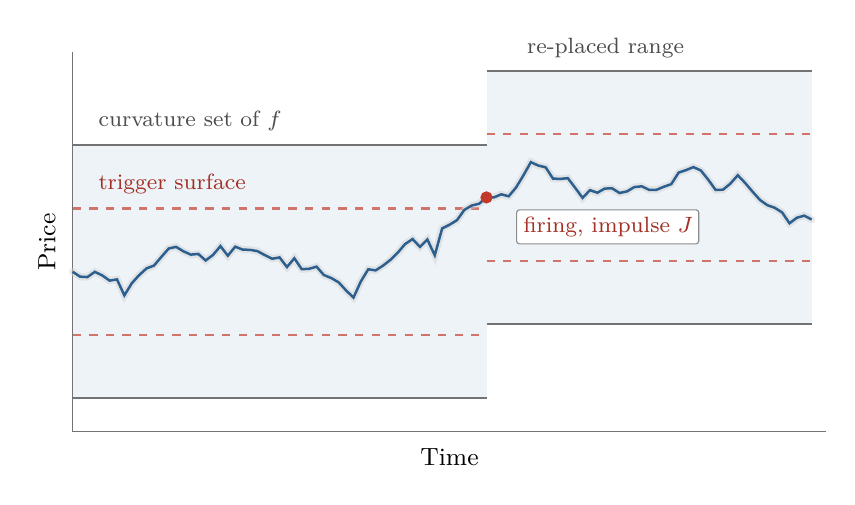
\begin{tikzpicture}
\begin{axis}[
  ltaxis,
  width=0.92\linewidth, height=6.4cm,
  xmin=0, xmax=1.02, ymin=0.12, ymax=1.02,
  xlabel={Time}, ylabel={Price},
  xtick=\empty, ytick=\empty,
  clip=false,
]
% the deployed range, tinted so the re-placement is visible as a shift
\path[fill=ltbandtint] (axis cs:0,0.20) rectangle (axis cs:0.56,0.80);
\path[fill=ltbandtint] (axis cs:0.56,0.3762) rectangle (axis cs:1.0,0.9762);
% range 1 bounds (curvature set) and trigger surfaces
\addplot[black!55, thick, domain=0:0.56, samples=2, forget plot] {0.80};
\addplot[black!55, thick, domain=0:0.56, samples=2, forget plot] {0.20};
\addplot[ltred!70, thick, dashed, domain=0:0.56, samples=2, forget plot] {0.65};
\addplot[ltred!70, thick, dashed, domain=0:0.56, samples=2, forget plot] {0.35};
% range 2 after the firing
\addplot[black!55, thick, domain=0.56:1.0, samples=2, forget plot] {0.9762};
\addplot[black!55, thick, domain=0.56:1.0, samples=2, forget plot] {0.3762};
\addplot[ltred!70, thick, dashed, domain=0.56:1.0, samples=2, forget plot] {0.8262};
\addplot[ltred!70, thick, dashed, domain=0.56:1.0, samples=2, forget plot] {0.5262};
% the price path
\addplot[ltblue, line width=0.9pt, ltglow, forget plot] coordinates {
(0.0,0.5) (0.01,0.4882) (0.02,0.4872) (0.03,0.4996) (0.04,0.4913)
(0.05,0.4788) (0.06,0.4817) (0.07,0.4438) (0.08,0.4724) (0.09,0.4919)
(0.1,0.5078) (0.11,0.5144) (0.12,0.5349) (0.13,0.555) (0.14,0.5589)
(0.15,0.5482) (0.16,0.5405) (0.17,0.5421) (0.18,0.5266) (0.19,0.5398)
(0.2,0.5607) (0.21,0.5379) (0.22,0.5594) (0.23,0.5524) (0.24,0.5518)
(0.25,0.5488) (0.26,0.5394) (0.27,0.5307) (0.28,0.5338) (0.29,0.511)
(0.3,0.5318) (0.31,0.5059) (0.32,0.5069) (0.33,0.5119) (0.34,0.492)
(0.35,0.4849) (0.36,0.4746) (0.37,0.4556) (0.38,0.4385) (0.39,0.477)
(0.4,0.5057) (0.41,0.5031) (0.42,0.5144) (0.43,0.528) (0.44,0.5453)
(0.45,0.5658) (0.46,0.5774) (0.47,0.5588) (0.48,0.5762) (0.49,0.539)
(0.5,0.6026) (0.51,0.6114) (0.52,0.6221) (0.53,0.6465) (0.54,0.657)
(0.55,0.6612) (0.56,0.6762)
};
\addplot[ltblue, line width=0.9pt, ltglow, forget plot] coordinates {
(0.56,0.6762) (0.57,0.6762) (0.58,0.6835) (0.59,0.6789) (0.6,0.6997)
(0.61,0.7286) (0.62,0.7599) (0.63,0.7518) (0.64,0.7475) (0.65,0.7208)
(0.66,0.7201) (0.67,0.7219) (0.68,0.6989) (0.69,0.6751) (0.7,0.6934)
(0.71,0.6873) (0.72,0.6972) (0.73,0.6977) (0.74,0.6867) (0.75,0.6904)
(0.76,0.7007) (0.77,0.7025) (0.78,0.6942) (0.79,0.6942) (0.8,0.7015)
(0.81,0.7077) (0.82,0.7351) (0.83,0.741) (0.84,0.7481) (0.85,0.7401)
(0.86,0.7183) (0.87,0.6939) (0.88,0.6945) (0.89,0.7089) (0.9,0.7288)
(0.91,0.7104) (0.92,0.6898) (0.93,0.6702) (0.94,0.6577) (0.95,0.6516)
(0.96,0.6405) (0.97,0.6148) (0.98,0.628) (0.99,0.6329) (1.0,0.6237)
};
% firing marker
\addplot[only marks, mark=*, mark size=2pt, ltred, forget plot]
  coordinates {(0.56,0.6762)};
% annotations
\node[font=\footnotesize, anchor=south west, black!70] at
  (axis cs:0.02,0.807) {curvature set of $f$};
\node[font=\footnotesize, anchor=south west, text=ltred!85!black] at
  (axis cs:0.02,0.657) {trigger surface};
\node[ltcallout, anchor=north west, text=ltred!85!black] at
  (axis cs:0.60,0.648) {firing, impulse $J$};
\node[font=\footnotesize, anchor=south west, black!70] at
  (axis cs:0.60,0.980) {re-placed range};
\end{axis}
\end{tikzpicture}
\caption{The controlled pair in the concentrated liquidity
instance. The price path accumulates local time against the bounds
of the deployed range (solid, tinted), the curvature set of $f$; a
crossing of a trigger surface (dashed) fires the impulse, which
surrenders $J$ and re-places the range.}
\label{fig:object}
\end{figure}

% =========================================================================
\section{The equidistribution lemma}\label{sec:lemma}

Both floors of the corpus consume one distributional input, the
uniformity of a sampled state modulo a grid. A sampling density
suffices.

\begin{lemma}[Offset Uniformity]\label{lem:offset}
Let $Z$ be a real random variable whose law has a density $q$ of
finite total variation $\mathrm{TV}(q)$, the variation of the density
as a function of the price rather than of the signed measure it
carries. Then the law of
$\zeta_\vartheta(Z)$ on $[0,1)$ has a density $\bar p_\vartheta$ with
\[
\sup_{z \in [0,1)} \big| \bar p_\vartheta(z) - 1 \big| \;\le\;
\vartheta\, \mathrm{TV}(q),
\]
and total-variation distance between laws at most $\vartheta\,
\mathrm{TV}(q)/2$ from the uniform law.
\end{lemma}

\begin{proof}[Proof sketch]
An oscillation bound on the pushforward density against the total
variation of $q$; Appendix~\ref{app:intensity}.
\end{proof}

\begin{lemma}[Conditional Offset Uniformity]\label{lem:conditional}
Let $\mathcal{G}$ be a sub-$\sigma$-algebra such that a regular
conditional density $q_{\mathcal{G}}$ of $Z$ given $\mathcal{G}$
exists with $\mathrm{TV}(q_{\mathcal{G}}) \le v$ almost surely. Then
the bound of Lemma~\ref{lem:offset} holds conditionally, and for
bounded measurable $g$ on $[0,1)$ and bounded
$\mathcal{G}$-measurable $Y$,
\[
\Big| \mathbb{E}\big[ g(\zeta_\vartheta(Z))\, Y \big] -
\Big(\int_0^1 g\Big)\, \mathbb{E}[Y] \Big| \;\le\; \tfrac12\,
\vartheta\, v\, \|g\|_\infty \|Y\|_\infty .
\]
\end{lemma}

\begin{proof}
Apply Lemma~\ref{lem:offset} under the regular conditional density,
pointwise in $\omega$, and integrate.
\end{proof}

The conditional form is the working tool. It makes the offset
approximately independent of every coarse-scale variable, with the
error of that approximation bounded by $\vartheta v$, which is how
the independence assumption of the value channel becomes a
quantified conclusion in Section~\ref{sec:red-value}.

\begin{corollary}[Occupation Sampling]\label{cor:occupation}
Let $\hat X$ be the quadratic-variation sampling of the path over
$[0,T]$, defined by
\[
\mathbb{P}(\hat X \in A) \;=\;
\frac{\mathbb{E}\int_0^T \mathbf{1}_A(X_s)\, d\langle X \rangle_s}
{\mathbb{E}\langle X \rangle_T}.
\]
If $\psi_T$ has finite total variation then
$\zeta_\vartheta(\hat X)$ is uniform to
\[
\sup_{z}\, \big|\bar p_\vartheta(z) - 1\big| \;\le\;
\frac{\vartheta\, \mathrm{TV}(\psi_T)}{\mathbb{E}\langle X \rangle_T}.
\]
\end{corollary}

The sampling here is by occupation. Offsets sampled at firings are a
different object, taken up at the end of the section.

For Brownian motion in the tick coordinate, $X = \sigma B$ from the
origin, $\psi_T$ is even and unimodal with $\mathrm{TV}(\psi_T) =
2\psi_T(0) = 2\sigma\sqrt{2T/\pi}$ and $\mathbb{E}\langle X\rangle_T =
\sigma^2 T$, so the deviation from uniformity is at most
$1.60\, \vartheta / (\sigma \sqrt T)$, the constant being
$2\sqrt2/\sqrt\pi$. The same constant bounds the drifted
era model, since the total variation of a Gaussian mixture does not
see the means (Lemma~\ref{lem:psireg}), so the corollary needs no
driftless assumption. The single knob is grid spacing over the
diffusive range of the window. On OQM's production panel the tick
series wanders hundreds of ticks per sampling window, so the tick-grid
instance is uniform to well under a per cent, matching the observed
near-uniformity of the within-tick offset, while the spacing-grid
instance carries a constant one to two orders larger. The latter
predicts that the placement-wedge fit should sit slightly below its
ideal slope in pools where overshoot spread is not large against the
spacing, which is consistent with OQM's reported slope of 0.94; a
per-pool test of this attenuation is left to future empirical work.

The pathwise analogue replaces $\psi_T$ with the realised field $a
\mapsto \ell_T^a$, which is not of finite variation, so the
oscillation argument runs cell by cell against its modulus of
continuity and yields an error of order $\vartheta^{1/2-\varepsilon}$
with a random constant for Brownian-type
laws.\cite{revuzyor,trotter1958} The mean form above is the one that
expected flux consumes.

The
empirical offsets of the corpus are sampled at firings, and a
continuous price monitored continuously fires exactly on its trigger
line, so the firing-state offset is a point mass and no uniformity of
any kind holds. Deployed systems observe the price on a keeper
cadence; the firing state overshoots the line with a conditional
density whose scale is set by $\sigma\sqrt{\Delta t}$ over one check
interval, and Lemma~\ref{lem:conditional} applies to that density.
Uniformity at firings is therefore a joint property of the price law
and the monitoring process, quantified in
Section~\ref{sec:extensions}, and it degrades as monitoring approaches
continuity, a prediction testable on
existing data across operators of known cadence.

% =========================================================================
\section{The forward identity}\label{sec:identity}

\subsection{The pathwise dissipation identity}\label{sec:pathwise}

The frame is one identity, exact on paths, whose only inputs are
the controlled pair and the convexity structure of the holding
value.

\begin{theorem}[Dissipation Identity]\label{thm:dissipation}
Let $X$ be a continuous semimartingale, $\mathcal{V}$ a venue
presentation with $f(\cdot, R)$ a difference of convex functions for
each $R$, and let the controlled pair satisfy uniform interior
placement and conservative emission \eqref{eq:conservative}. Then
almost surely, for every $T \ge 0$,
% One line: the stochastic integral carries its endpoints as limits
% rather than as an interval subscript, which is 24pt narrower and
% brings the display back inside the measure with room for the number.
% \vphantom equalises the three brace-label depths.
\begin{equation}\label{eq:dissipation}
\sum_{k:\, \tau_k \le T} J_k
\;=\; \underbrace{f(X_0, R_0) - f(X_T, R_T)
  \vphantom{\int_{\tau_k \wedge T}^{\tau_{k+1} \wedge T}}
  }_{\textnormal{boundary}}
\;+\; \underbrace{\sum_k \int_{\tau_k \wedge T}^{\tau_{k+1} \wedge T}
f'_-(X_s, R_k)\, dX_s}_{\textnormal{martingale}}
\;+\; \underbrace{\tfrac12 \sum_k \int_{\mathbb{R}}
\Delta_k \ell^a_T \,f''_{R_k}(da)
  \vphantom{\int_{\tau_k \wedge T}^{\tau_{k+1} \wedge T}}
  }_{\textnormal{local time}},
\end{equation}
where $\Delta_k \ell^a_T = \ell^a_{\tau_{k+1} \wedge T} -
\ell^a_{\tau_k \wedge T}$ is the local time accrued on the $k$-th
inter-firing interval. The accrual channel, when present, adds
$\int_0^T c(X_s, R_s)\, ds$ to the left side with its occupation
representation on the right.
\end{theorem}

\begin{proof}
On each interval $[\tau_k, \tau_{k+1})$ the policy state is frozen and
It\^o--Tanaka applies to $f(\cdot, R_k)$.\cite{revuzyor} At
$\tau_k$ the process $f(X_t, R_t)$ jumps by $f(X_{\tau_k},
R_k) - f(X_{\tau_k}, R_{k-1}) = -J_k$ by
\eqref{eq:conservative}. Telescoping over the finitely many firings on
$[0,T]$ gives \eqref{eq:dissipation}.
\end{proof}

\emph{In words, everything the policy surrenders at its firings is the
decline in holding value over the window, plus what the price path
contributes between firings, adjusted by the curvature the price
accumulates where the holding value bends.} The identity is exact and pathwise; every
probabilistic statement below evaluates the expectations of its
terms. Taking expectations with $X$ a local
martingale on the era and enough integrability for the stochastic
integral to vanish in mean, for which it suffices that $f'_-$ is
bounded on the price interval the stopped era path visits and
$\mathbb{E}\langle X \rangle_T < \infty$
(Appendix~\ref{app:intensity}),
\begin{equation}\label{eq:mean}
\mathbb{E} \sum_{\tau_k \le T} J_k
\;=\; \mathbb{E}\big[ f(X_0, R_0) - f(X_T, R_T) \big]
\;+\; \tfrac12\, \mathbb{E} \sum_k \int \Delta_k \ell^a_T\,
f''_{R_k}(da).
\end{equation}

\begin{remark}[The Two Cost Layers]\label{rem:layers}
In the concentrated liquidity instance the in-range part of the
local-time term prices the occupation of a concave payoff by a
diffusing price, which is the slot occupied by
loss-versus-rebalancing;\cite{milionis2022} the definitions differ,
that cost being benchmark-relative, so no equivalence is claimed. The
impulse sum is the quantisation and execution flow of OQM. That
paper kept the two layers orthogonal as a modelling discipline;
\eqref{eq:dissipation} derives the orthogonality, the layers being
distinct terms of one expansion, so neither can double-count the
other.
\end{remark}

\subsection{The intensity representation}\label{sec:intensity}

The era model makes the impulse term computable; the proposition
assembles four ingredients, a renewal structure, a direction law, a
firing-state law, and the resulting flux rate. Let $X_t = \mu t +
\sigma B_t$ in tick units with era-constant parameters, let the
policy be the concentrated liquidity instance with trigger distances
$w_u, w_d$ from the placement point, and let monitoring follow
Section~\ref{sec:extensions}.

\begin{proposition}[Intensity Representation]\label{prop:intensity}
Under the era model,
\begin{enumerate}[label=(\roman*)]
\item inter-firing cycles are independent and identically distributed
given the era, and $N_T / T \to \lambda = 1/\mathbb{E}[\text{cycle
length}]$ almost surely;
\item the firing-direction probabilities $\pi^+ =
\mathbb{P}(\mathrm{up})$ and $\pi^- = \mathbb{P}(\mathrm{down})$
satisfy, with $\theta = 2\mu/\sigma^2$,
\[
\frac{\pi^+}{\pi^-} \;=\;
\frac{e^{\theta w_d} - 1}{1 - e^{-\theta w_u}},
\]
up to a monitoring correction bounded
in Proposition~\ref{prop:monitoring};
\item the state at firing is the trigger line plus an overshoot whose
conditional density satisfies the hypothesis of
Lemma~\ref{lem:conditional} at grid scale;
\item the era flux rate is
\[
\lambda\,\big( \pi^+\, \mathbb{E}[J \mid \mathrm{up}]
+ \pi^-\, \mathbb{E}[J \mid \mathrm{down}]\big),
\]
with the
conditional amplitudes computed by integrating the source-derived
amplitude against the offset and overshoot laws of (iii).
\end{enumerate}
\end{proposition}

\emph{In words, the era model turns the impulse term into a rate,
firing frequency times the direction-weighted mean amplitude, with
every factor computable from the source and the era parameters.} Item
(ii) coincides with the directional firing law of OQM. Writing $\Lambda$ for
the compensator of the firing counting process and $\tilde c$ for the
accrual rate metered in the quadratic-variation clock, the era-form
summary is
% Two lines by measurement: one line is 438.5pt of content against a
% 453.0pt measure and the number needs 18pt, so it cannot fit without
% cramping. The three right-hand terms are only 306pt together, so
% they go below the left-hand side as one uninterrupted sum rather
% than being broken between terms. \gathered centres both lines, which
% keeps this display consistent with every other one in the paper, and
% centres the number vertically.
% The \textstyle must be braced: as a bare switch it ran to the end of
% the display and set every operator on the right in text size.
\begin{equation}\label{eq:forwardlaw}
\begin{gathered}
\mathbb{E}\Big[ \Phi_T + {\textstyle\int_0^T} c(X_s, R_s)\, ds \Big]
\;=\; \\[4pt]
\underbrace{\int_{\mathbb{R}} \tilde c(a)\, \psi_T(a)\,
da}_{\textnormal{occupation}}
\;+\; \underbrace{\tfrac12\, \mathbb{E} \sum_k \int \Delta_k \ell^a_T\,
f''_{R_k}(da)}_{\textnormal{local time}}
\;+\; \underbrace{\mathbb{E} \int_0^T J(X_t, R_{t-})\,
d\Lambda_t}_{\textnormal{firing intensity}} ,
\end{gathered}
\end{equation}
expected flux as amplitude integrated against the three carriers named
beneath it, with Proposition~\ref{prop:intensity} evaluating $\Lambda$
for the era model. Equating the impulse-term evaluations of \eqref{eq:mean} and
\eqref{eq:forwardlaw} is the bridge between occupation of the
discontinuity set and firing intensity; OF's identification argument,
that firing intensity is occupation density times hazard, is the
folded-coordinate form of this bridge.

The right side of \eqref{eq:forwardlaw} localises in price, and the
localisation is the paper's organising object.

\begin{definition}[Dissipation Measure]\label{def:ximeasure}
For a venue presentation, an era, and a horizon $T$, the
dissipation measure $\Xi_T$ assigns to a Borel set $A$ the expected
flux generated at price levels in $A$, the three carriers of
\eqref{eq:forwardlaw} restricted to $A$ in the same order,
\[
\Xi_T(A) \;=\; \int_A \tilde c(a)\, \psi_T(a)\, da
\;+\; \tfrac12\, \mathbb{E} \sum_k \int_A \Delta_k \ell^a_T\,
f''_{R_k}(da)
\;+\; \mathbb{E} \int_0^T \mathbf{1}\{X_{t-} \in A\}\,
J(X_t, R_{t-})\, d\Lambda_t .
\]
\end{definition}

The middle carrier is signed. A concentrated liquidity holding value
is concave in the square-root price coordinate, so $f''_R$ is a
negative measure there and the local-time term is a credit against
the other two rather than a charge beside them; the concavity leg's
cost is its negative, which is the sign in which the benchmark
literature reports the same quantity. $\Xi_T$ is a signed measure,
and its total mass is an expected flux, not a sum of
non-negative parts.

The forward law is the statement that expected total flux is
$\Xi_T(\mathbb{R})$. Only the impulse carrier sits on
$\mathcal{D}(R)$ exactly, on the trigger surfaces where firings
occur. The other two sit on the supports of their densities, and
$\mathcal{D}_c$ and $\mathcal{D}_f$ record where those densities
break rather than where they live. How much larger the supports are
is a property of the venue class. In the V3 geometry the accrual rate
vanishes identically and $f''_R$ is an interval density that is
piecewise constant, so the local-time carrier contributes a smooth
background whose only structure, the jumps of that density, sits on
$\mathcal{D}_f$; in the discrete-bin geometry of
Appendix~\ref{app:lb} the second-derivative measure is purely atomic
and its carrier sits on $\mathcal{D}_f$ entirely, while the per-bin
fee credit puts the accrual carrier on the occupied bin. Dissipation
living on the code's discontinuity set is therefore exact for a
discrete-bin venue and exact up to a smooth background for a V3 one.
The second act bounds the impulse component from below per unit time
over policy classes, and the third act's instrument identifies the
jump part of that component from firing data.

\subsection{The central law}\label{sec:centrallaw}

The impulse amplitudes that $\Xi_T$ integrates are not modelling
inputs. In the concentrated liquidity instance they obey an exact
law in one state variable, the paper's central result, stated here
with the frame because everything that follows consumes it. GS's
Theorem~1 characterised when the re-placement cost vanishes; the
law states what the cost is, always, at any width pair, the floors
of the second act are its global consequence, and the jump
surcharge prices jump crossings through its potentials.

Work in the sqrt-price coordinate of Section~\ref{sec:venue}. A
position $(L, [s_a, s_b])$ with the price $s$ in range has
withdrawable amounts $x = L(1/s - 1/s_b)$ and $y = L(s - s_a)$ and
value $V = x s^2 + y$ in token1 units, the $L\,\phi$ of
Section~\ref{sec:venue}. The holdings shares are
\begin{equation}\label{eq:shares}
\omega_0 \;=\; \frac{x\,s^2}{V}, \qquad \omega_1 \;=\; \frac{y}{V}
\;=\; 1 - \omega_0,
\end{equation}
the token0 and token1 value shares of the withdrawn position. Writing
$(x_u, y_u)$ for a candidate range's per-liquidity amounts at the same
price, its \emph{target shares} are the same formula applied to
those, $\omega_0' = x_u s^2/(x_u s^2 + y_u)$ and $\omega_1' = y_u/(x_u
s^2 + y_u)$. The share $\omega_0$ is OQM's
token0 value share, promoted from bookkeeping to state variable. An
isolated re-placement withdraws $(x, y)$ at price $s$ and re-mints
into an admissible range containing $s$ through the binding-side
minimum $L' = \min(x/x_u,\, y/y_u)$, emitting the non-binding surplus
per \eqref{eq:conservative}. Writing $V'$ for the value of the re-minted
position at the same price, its mint kerf is the log-cost
\begin{equation}\label{eq:kdef}
k \;=\; -\ln \frac{V'}{V} .
\end{equation}
The kerf is a log cost, and the flux it surrenders is exactly $J = V
- V' = V(1 - e^{-k})$. Since $1 - e^{-k} \le k$, the log cost
dominates the value fraction and the two agree only to first order.
Everything below is stated in log units, kerfs, rates, and floors
alike, so a value-fraction rate from another source is not directly
comparable.

\begin{theorem}[Share-Potential Identity]\label{thm:share}
For an isolated re-placement at price $s$, from any range containing
$s$ to any admissible range containing $s$, at any width pair, with
holdings shares $(\omega_0, \omega_1)$ and target shares
$(\omega_0', \omega_1')$ as in \eqref{eq:shares},
\begin{equation}\label{eq:shareid}
k \;=\; \max\!\Big( \ln \frac{\omega_0'}{\omega_0},\;
\ln \frac{\omega_1'}{\omega_1} \Big).
\end{equation}
In particular $k \ge 0$ always, with $k = 0$ exactly when the target
shares equal the holdings shares.
\end{theorem}

\begin{proof}[Proof sketch]
If the token0 constraint binds, $L' = x/x_u$ and the retained value
fraction is $(x/x_u)(x_u s^2 + y_u)/V = \omega_0 / \omega_0'$;
symmetrically the token1 branch retains $\omega_1/\omega_1'$. The
mint takes the minimum of the two, so the retained fraction is
$\min(\omega_0/\omega_0',\, \omega_1/\omega_1')$, and
\eqref{eq:shareid} is its negative logarithm. Full algebra in
Appendix~\ref{app:cost}.
\end{proof}

\emph{In words, for an isolated re-placement the mint kerf is exactly
the price of moving the position's composition; width, centring, and
the price level enter only through the shares.} The venue-wide ledger
of Definition~\ref{def:ximeasure} is signed and has three carriers;
this is the one that is non-negative and event-level. Its zero set
carries the first consequence.

\begin{corollary}[Free Locus]\label{cor:free}
The kerf vanishes exactly on the share-preserving re-placements, at
every width. These are GS's ratio-preserving locus, the zero-kerf
set; they do not touch the holdings, and therefore do not move
$\omega_0$.
\end{corollary}

Corollary~\ref{cor:free} settles the free-riding question, whether
a policy can translate its centre along the free locus and track
the price without paying. Centre motion is not the charged
variable. In the isolated arithmetic a policy may slide and widen
without paying a kerf, since its composition does not move, and every
bound below charges composition motion alone. A deployed policy still
pays gas, fees, and any corrective swap, which the swap class of
Section~\ref{sec:swap} prices separately. The second act works in the law's potential form
(Corollary~\ref{cor:family}), and the two-branch closed form of the
next section is its boundary case $\delta' = 0$.

% =========================================================================
\section{The amplitude layer}\label{sec:red-amplitude}

The first of three specialisations narrows the central law to one
geometry, the isolated equal-width rebalance that recentres the range
on the current price. Throughout, the old range is $[s_a, s_b]$ in
sqrt price with half-width $h$ and midpoint $\bar s$, the current
sqrt price is $s = \bar s + \delta$ with $|\delta| \le h$, and the
new range is $[s - h, s + h]$. The amplitude is the value surrendered
at the event,
\[
\Delta R(\delta) \;=\; V_{\mathrm{old}}(s) - V_{\mathrm{new}}(s)
\;\ge\; 0 ,
\]
in token1 units, which is the geometric residual of GS in the
value-surrendered sign convention adopted throughout. It carries the
same content as the kerf of \eqref{eq:kdef} in different units,
$k = -\ln(1 - \Delta R / V_{\mathrm{old}})$, and the floors of the
second act work in $k$; nothing in this section is yet a bound.
The amplitude is the boundary case $\delta' = 0$ of the central law's
potentials (Corollary~\ref{cor:family}).

The down-branch geometry below is not new in substance. OQM's
swap-free credit publishes the token0 form of the lower branch, its
sign corollary states the corner ratio, and the concurrent preprint of
I.\,P.\cite{pi2026convexity} derives the same credits independently.
This section adds the assembly, the two-branch closed form in the
value-surrendered frame of GS, the bridge to GS's mint-minimum
development, the reconciliation of the two published boundary factors,
and a monotonicity threshold that neither paper states. Proofs are in
Appendix~\ref{app:amplitude}.

\begin{lemma}[Binding Side]\label{lem:binding}
In the mint minimum the token1 term binds exactly when $\delta \le 0$
and the token0 term exactly when $\delta \ge 0$.
\end{lemma}

\begin{proposition}[Two-Branch Amplitude]\label{prop:amplitude}
The value surrendered by the equal-width recentred rebalance is
\begin{equation}\label{eq:branches}
\Delta R(\delta) \;=\;
\begin{cases}
\dfrac{L\,\delta\,(2\bar s + h + \delta)}{\bar s + h},
& 0 \le \delta \le h,\\[10pt]
\dfrac{-L\,\delta\,(\bar s + \delta)\,(2\bar s + h + \delta)}
{(\bar s + h)(\bar s + h + \delta)},
& -h \le \delta \le 0,
\end{cases}
\end{equation}
and the two branches satisfy $\Delta R_{\downarrow}(\delta) =
|\Delta R_{\uparrow}^{\mathrm{cont}}(\delta)| \cdot s / s_b'$, where
$\Delta R_{\uparrow}^{\mathrm{cont}}$ is the upper branch continued to
$\delta < 0$ and $s_b' = s + h$ is the new range's upper bound.
\end{proposition}

\begin{corollary}[Corner Values]\label{cor:corners}
At the range corners the mint is empty and the amplitude equals the
entire corner position value,
\[
\Delta R(h) = V(s_b) = L\,w, \qquad
\Delta R(-h) = V(s_a) = L\,w\,\frac{s_a}{s_b}, \qquad w = 2h .
\]
The boundary asymmetry factor is $s_a / s_b$, the corner ratio of
OQM's sign corollary; the factor $\bar s / s_b$ stated in GS is the
interior limit $\Delta R_{\downarrow}(m)/\Delta R_{\uparrow}(m) \to
\bar s / s_b$ as $m = |\delta| \to 0^+$, consistent with GS's
directional identity.
\end{corollary}

\begin{proposition}[Down-Branch Monotonicity]\label{prop:mono}
$\Delta R_{\downarrow}$ is strictly increasing in $|\delta|$ on $(0,
h]$ if and only if $h / \bar s \le (\sqrt{17} - 3)/2$, equivalently
$s_b / s_a \le (3 + \sqrt{17})/2 \approx 3.562$. Above the threshold
the down branch attains an interior maximum and decreases to the
corner value.
\end{proposition}

\emph{In words, the value a recentred rebalance surrenders is a
two-branch closed form in the displacement, the two published
boundary factors are two limits of that one function, and the down
branch is monotone exactly on one side of an explicit width
threshold, the side the deployed ranges sit on.}

Figure~\ref{fig:branches} plots both branches for a narrow and a wide
range. The gap between the exact down branch and the continuation, and
the turnover above the threshold, are shown; the markers at the left
edge are the two corner values.\footnote{As published, GS's
monotonicity theorem asserts both branches strictly monotone with no
width hypothesis, and Proposition~\ref{prop:mono} supplies the
condition the down branch needs. Production ranges sit one to two
orders inside the threshold, so the empirical content of GS is
unaffected.}

\begin{figure}[H]
\centering
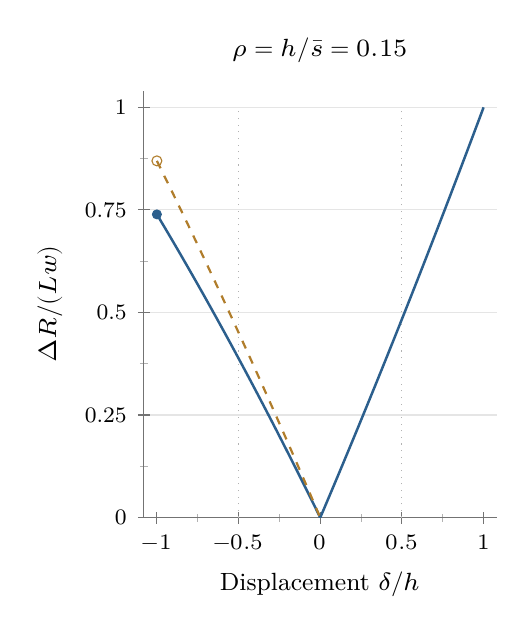
\begin{tikzpicture}
\begin{axis}[
  ltaxis,
  width=0.50\linewidth, height=7cm,
  xmin=-1.08, xmax=1.08, ymin=0, ymax=1.04,
  xlabel={Displacement $\delta/h$}, ylabel={$\Delta R / (Lw)$},
  xtick={-1,-0.5,0,0.5,1}, ytick={0,0.25,0.5,0.75,1},
  yticklabels={0,0.25,0.5,0.75,1},
  minor x tick num=1, minor y tick num=1,
  title={$\rho = h/\bar s = 0.15$},
  ymajorgrids,
]
\addplot[black!30, dotted, forget plot] coordinates {(-0.5,0) (-0.5,1)};
\addplot[black!30, dotted, forget plot] coordinates {(0.5,0) (0.5,1)};
\addplot[ltblue, line width=0.9pt, domain=0:1, samples=60, forget plot]
  {x*(2+0.15+x*0.15)/(2*(1+0.15))};
\addplot[ltblue, line width=0.9pt, domain=-1:0, samples=80, forget plot]
  {-x*(1+x*0.15)*(2+0.15+x*0.15)/(2*(1+0.15)*(1+0.15+x*0.15))};
\addplot[ltamber, line width=0.8pt, dashed, domain=-1:0, samples=60, forget plot]
  {-x*(2+0.15+x*0.15)/(2*(1+0.15))};
\addplot[only marks, mark=*, mark size=1.6pt, ltblue, forget plot]
  coordinates {(-1,0.73913)};
\addplot[only marks, mark=o, mark size=1.8pt, ltamber, forget plot]
  coordinates {(-1,0.86957)};
\end{axis}
\end{tikzpicture}\hfill
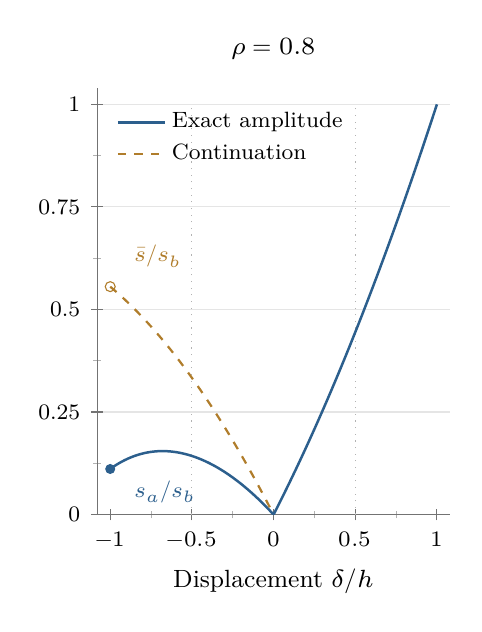
\begin{tikzpicture}
\begin{axis}[
  ltaxis,
  width=0.50\linewidth, height=7cm,
  xmin=-1.08, xmax=1.08, ymin=0, ymax=1.04,
  xlabel={Displacement $\delta/h$},
  xtick={-1,-0.5,0,0.5,1}, ytick={0,0.25,0.5,0.75,1},
  yticklabels={0,0.25,0.5,0.75,1},
  minor x tick num=1, minor y tick num=1,
  title={$\rho = 0.8$},
  ymajorgrids,
  legend style={font=\footnotesize, draw=none, fill=none,
    at={(0.03,0.97)}, anchor=north west},
  legend cell align=left,
]
\addplot[black!30, dotted, forget plot] coordinates {(-0.5,0) (-0.5,1)};
\addplot[black!30, dotted, forget plot] coordinates {(0.5,0) (0.5,1)};
\addplot[ltblue, line width=0.9pt, domain=0:1, samples=60]
  {x*(2+0.8+x*0.8)/(2*(1+0.8))};
\addlegendentry{Exact amplitude}
\addplot[ltblue, line width=0.9pt, domain=-1:0, samples=80, forget plot]
  {-x*(1+x*0.8)*(2+0.8+x*0.8)/(2*(1+0.8)*(1+0.8+x*0.8))};
\addplot[ltamber, line width=0.8pt, dashed, domain=-1:0, samples=60]
  {-x*(2+0.8+x*0.8)/(2*(1+0.8))};
\addlegendentry{Continuation}
\addplot[only marks, mark=*, mark size=1.6pt, ltblue, forget plot]
  coordinates {(-1,0.11111)};
\addplot[only marks, mark=o, mark size=1.8pt, ltamber, forget plot]
  coordinates {(-1,0.55556)};
\node[anchor=west, font=\footnotesize, text=ltblue]
  at (axis cs:-0.92,0.055) {$s_a/s_b$};
\node[anchor=west, font=\footnotesize, text=ltamber]
  at (axis cs:-0.92,0.63) {$\bar s/s_b$};
\end{axis}
\end{tikzpicture}
\caption{Two-branch amplitude \eqref{eq:branches} against normalised
displacement, for a narrow range (left) and a wide range (right).
Solid, the exact amplitude; dashed, the continuation of the up-branch
closed form; dotted verticals, the trigger displacement at $\varphi =
1/4$.}
\label{fig:branches}
\end{figure}

The vanishing condition of GS's first theorem enters the present
framework as the characterisation of the amplitude's null set, the
ratio-preserving locus. The amplitude's sign needs no separate
argument, both branches of \eqref{eq:branches} being manifestly
non-negative on their stated domains; it was nonetheless established
independently, as the machine-checked non-positivity of the
isolated-case residual in GS's companion
formalisation.\footnote{The formalisation ships in the GS repository
(\texttt{g4nc0r/the-geometric-siphon}, directory \texttt{lean/}),
machine-checked against a pinned mathlib; the GS paper itself predates
it. A citable archive reference is deferred to release.} Evaluating \eqref{eq:branches} at the trigger
displacement $\delta = (1 - 2\varphi) h$ plugs the amplitude layer
into Proposition~\ref{prop:intensity}(iv). The same displacement is
written $xh$ in the floor act's policy families, so the contract
fraction, the policy variable, and the displacement are one
quantity, $xh = (1 - 2\varphi)\,h$.

% =========================================================================
\section{The recovered channels}\label{sec:red-frequency}\label{sec:red-value}

The second and third specialisations are consistency checks; each
recovers a published channel law under the frame's hypotheses, and
neither is a claim that the published law holds without them. The
second is Proposition~\ref{prop:intensity}(ii), OQM's directional
firing law. The placement floor enters through the
barrier distances. The impulse map centres the new range at $\vartheta
\lfloor a / \vartheta \rfloor$ for spacing $\vartheta$, so the placed
midpoint sits below the firing tick by the placement offset $o =
\vartheta\, \zeta_\vartheta(a)$, the barriers become $w_u = \bar w +
o$ and $w_d = \bar w - o$, and the per-pool wedge in the log count
ratio is
\begin{equation}\label{eq:wedge}
\mathbb{E}\big[\log(w_d / w_u)\big] \;=\; -\,\mathbb{E}_o\left[
\log \frac{\bar w + o}{\bar w - o} \right],
\qquad o \sim U[0, \vartheta),
\end{equation}
with uniformity of $o$ supplied by Lemma~\ref{lem:conditional} on the
spacing grid to the error of Section~\ref{sec:lemma}, which is the
coarser instance and carries the slope-attenuation prediction stated
there. Equation \eqref{eq:wedge} is the quantisation prediction whose
per-pool fit (correlation 0.82, slope 0.94) was reported by OQM; the
formula itself appears here.

The third concerns the sizing arithmetic, which at a firing
computes its target token0 share at the floor tick and executes at
the continuous price. OQM's surplus decomposition and tick-race
law, taken here as the source-derived amplitude, give the leftover
side as $\operatorname{sign}(\zeta + \Delta)$ and the credit as
$g\,|\zeta + \Delta|\, V$, with $\zeta$ the within-tick offset,
$\Delta$ the corrective swap's tick displacement, and $g$ the local
tick sensitivity of the target share, to the fee-and-rounding error
order carried there. The forward law adds the distributional layer.
The firing-state law of Proposition~\ref{prop:intensity}(iii)
satisfies the hypothesis of Lemma~\ref{lem:conditional} on the tick
grid, $\Delta$ is measurable to leading order with respect to the
coarse state, and therefore $\zeta$ is uniform and decoupled from
$\Delta$, both to the error of Lemma~\ref{lem:conditional}. The probabilities that the leftover lands
opposite the bought token, conditional on direction, follow as
\begin{equation}\label{eq:qmix}
q^+ = \mathbb{E}\big[ \min\big((-\Delta)_+,\, 1\big) \mid \mathrm{up}
\big], \qquad
q^- = \mathbb{E}\big[ \min\big((1 + \Delta)_+,\, 1\big) \mid
\mathrm{down} \big],
\end{equation}
with $z_+ = \max(z, 0)$, each expectation reading off the uniform
offset's chance of losing the race. What was an assumption block in OQM,
uniformity of $\zeta$ and its independence from $\Delta$, is now a
lemma plus a stated hypothesis on the firing law, and the empirical
checks there (near-uniform $\zeta$, rank correlations within $\pm
0.04$, $q^+$ of 0.06 to 0.10 against $q^-$ near 0.5) test the
hypothesis rather than stand in for a theorem.

% =========================================================================
% =========================================================================
\section{The recipe}\label{sec:recipe}

A new venue enters the forward law through
Definition~\ref{def:venue}. Read the policy state space, the accrual
rate, the holding value, the firing set, and the impulse map from
contract source; the discontinuity set and amplitudes follow, and
\eqref{eq:dissipation} and Proposition~\ref{prop:intensity} do the
rest. Discrete-bin designs place the grid in the holding value
itself, whose second-derivative measure is atomic at the bin prices
(Appendix~\ref{app:lb}), and venues with contract-encoded
movement modes make the firing set public, which permits exact
scoring of blind recovery. What the frame supplies is a fixed
interface; what a new venue costs is the slot filling, the event
reconstruction, and whatever its own geometry demands. The
discrete-bin case is the worked example of that last item, its atomic
second-derivative measure being a structure the V3 development never
needed.\footnote{Three further classes fill the
slots without new theory. Hook architectures put all five in
operator-authored code; repegging gates with hysteresis are firing
sets with state-dependent boundaries; and liquidation engines put
atoms in the holding value's second-derivative measure, lighting the
local-time channel directly rather than through impulses.} At the exact layer that claim now has an
executed instance; the fork suite of Section~\ref{sec:verification}
asserts the central law's arithmetic against a second unmodified
deployment of the V3 class, so the demonstrated content is
portability of the pipeline across deployments. At the venue-class
level, Appendix~\ref{app:lb} carries out the first non-V3
instantiation, reading the Trader Joe Liquidity Book through
Definition~\ref{def:venue} from contract source with a purely
atomic second-derivative measure, an instantiation asserted in
turn against the venue's unmodified home deployment
(Section~\ref{sec:verification}); the population read of a
discrete-bin venue remains open.


% =========================================================================
\section{Jump price laws and monitoring}\label{sec:extensions}\label{sec:instrumentresponse}

\subsection{Jump price laws}\label{sec:jumps}

For a semimartingale with jumps, Meyer--It\^o replaces It\^o--Tanaka
in Theorem~\ref{thm:dissipation}, and the right side of
\eqref{eq:dissipation} gains the jump-remainder sum
\[
\sum_s \big[ f(X_s) -
f(X_{s-}) - f'_-(X_{s-})\, \Delta X_s \big]
\]
over jump times, the local time being that of the continuous
part.\cite{protter2005} The sum is pathwise and uncompensated; under
the integrability of Section~\ref{sec:identity} its expectation is
evaluated through the compensator of the jump measure. A jump across
a boundary accumulates no local time and contributes through this
sum.
A jump across a trigger surface fires the impulse from the landing
point, so the firing compensator splits into a continuous-crossing
part, governed by first passage as above, and a jump-crossing part,
an integral of the jump measure over straddling jumps
(Appendix~\ref{app:intensity}). The overshoot past the trigger line
at firing is therefore an observable of the jump measure, once the
monitoring overshoot of the next subsection is accounted for. Reading
integrated jump-tail functionals from population overshoot data,
conditionally and per pool rather than recovering the measure itself,
is the inverse problem the third act pursues
(Sections~\ref{sec:instrument}--\ref{sec:evidence}).

\subsection{Monitoring}\label{sec:monitoring}

Deployed systems evaluate their firing condition at check times
$(t_j)$ and fire at the first check with $X_{t_j} \in F(R)$. The
proposition below is stated for check times independent of $X$,
deterministic cadence and Poisson checking both admitted; the
activity-dependent Cox case, in which the check intensity responds to
the observable state, is carried in the third act under the exclusion
restriction (F4) of Table~\ref{tab:hypotheses}. Three consequences
follow.

\begin{proposition}[Monitoring Layer]\label{prop:monitoring}
Under the era model with check interval $\Delta t$ and one-check
scale $\sigma_1 = \sigma\sqrt{\Delta t}$,
\begin{enumerate}[label=(\roman*)]
\item conditional on firing at a surface $b$, the firing state is $b +
O$ with the overshoot $O$ admitting, under the flat-entry hypothesis
of Appendix~\ref{app:intensity}, the density $\sqrt{2\pi}\,
\surv(o/\sigma_1)/\sigma_1$ with
$\surv$ the standard normal survival function, of total variation
$\sqrt{2\pi}/\sigma_1$ and mean $\approx
0.63\,\sigma_1$, so the offset-uniformity error at grid
$\vartheta$ is of order $\vartheta / \sigma_1$,
degrading to the degenerate trigger offset as $\Delta t \to 0$;
\item the realised firing intensity is, at leading order, that of the
continuous problem with each barrier shifted outward by
$\beta\,\sigma_1$ with $\beta \approx 0.5826$, the
continuity-correction constant of Broadie, Glasserman, and
Kou,\cite{bgk1997} a modest cadence thinning; where realised firing
rates sit well below the raw first-passage prediction, the gap is
carried by dead-band and dwell rules, which modify the firing set
rather than the monitoring;
\item the correction to the direction split of
Proposition~\ref{prop:intensity}(ii) is bounded by the probability of
an unobserved excursion to the opposite barrier within one check
interval, exponentially small in $(w_u + w_d)/(\sigma \sqrt{\Delta
t})$.
\end{enumerate}
\end{proposition}

\emph{In words, discrete monitoring makes every trigger-qualified
firing overshoot its line by a known density at the one-check scale,
thins the firing rate only mildly, and almost never records a firing
on the wrong side. Firings that a dwell or penetration rule has
filtered are not drawn from this kernel, which the third act
exploits.}

Item (i) is the structural fact announced in the introduction. The
grids the value channel is measured on come from placement and sizing
arithmetic, but the offset on them is random rather than degenerate
only because monitoring is discrete, and item (i) quantifies the
cadence prediction of Section~\ref{sec:lemma}. Item
(iii) is why slope-one fits of the directional law survive on
production data whose levels are heavily
thinned.\footnote{The same discreteness has been priced on the other
leg. Fixed block intervals admit a closed-form per-block benchmark
loss, and constant spacing minimises it over inter-block timing
patterns\cite{nezlobin2025}; here discreteness of observation moves
the event leg instead, and moves it upward.}


\actdivider{Act II}{The Floor}

\noindent\emph{The second act prices every admissible policy from
below. The central law makes each re-placement a potential
difference in the composition coordinate, so keeping a price in a
band has a running cost no policy design evades; three floors state
it, and one architecture deletes it. The act consumes the first
act's law and geometry, and deployed observation returns in the
menu and cadence terms.}

% =========================================================================
\section{Policies, classes, and the functional}\label{sec:classes}\label{sec:floor}

The second act bounds from below the kerf a policy accumulates per
unit time, over a base class and its two independent instrument
enrichments, and then treats a fourth architecture that changes the surplus rule rather
than the instrument set. The functional is the impulse leg of the
dissipation measure (Definition~\ref{def:ximeasure}) in log units
rather than in value units, a distinction
Section~\ref{sec:policies} makes exact.

\subsection{Setting}\label{sec:setup}

Work per era, on the filtered space of Section~\ref{sec:price}, in
the sqrt-price coordinate, where the mint geometry and the
composition share of Section~\ref{sec:centrallaw} are native. Within an era the sqrt price $s_t$ is a continuous local
martingale with $d\langle s \rangle_t = \sigma_s^2\, dt$ and
$\sigma_s$ era-constant, confined to the era band $[s_-, s_+]$, a
deterministic interval carried as era data and containing every
value the stopped era path visits; the integrability convention of
Section~\ref{sec:identity} holds on it. Monitoring is
continuous; the cadence layer returns in
Proposition~\ref{prop:cadence}. A position is a pair $(L, [s_a,
s_b])$ with the price in range, with withdrawable amounts, value,
and holdings shares $(\omega_0, \omega_1)$ as in
Section~\ref{sec:centrallaw}. The narrow-range parameter is
$\rho = h/\bar s$ for a range of half-width $h$ and midpoint $\bar
s$; statements invoking the narrow limit $\rho \to 0$ say so, and
the standing hypothesis $h/s_- \le 1/5$ is assumed throughout the
floor sections.

The state coordinate of the second act is the share $\omega_0$ of
\eqref{eq:shares}; between firings it evolves continuously with the
price and is strictly decreasing in $s$, and in the narrow limit
$\omega_0 \approx (s_b - s)/(s_b - s_a)$.

\subsection{Policies and cost}\label{sec:policies}

\begin{definition}[Policy and Kerf Rate]\label{def:policy}
A policy is a sequence of stopping times $\tau_1 < \tau_2 < \cdots$,
locally finite, and $\mathcal{F}_{\tau_j}$-measurable re-placement
choices. At $\tau_j$ the position is withdrawn and re-minted per
the isolated re-placement of Section~\ref{sec:centrallaw}, at
per-event kerf $k_j$ as in \eqref{eq:kdef}, non-negative by
Theorem~\ref{thm:share}. The kerf rate of the policy is its
accumulated kerf per unit time,
\begin{equation}\label{eq:rdef}
r \;=\; \limsup_{T \to \infty}\; \frac{1}{T}\, \mathbb{E}
\sum_{\tau_j \le T} k_j .
\end{equation}
\end{definition}

The log form compounds, and the numerical harness measures it. The
mean identity \eqref{eq:mean} prices the
impulse leg in value units, $\mathbb{E}\sum J_j$ with $J_j = g_j
V_{\tau_j-}$ and $g_j = 1 - e^{-k_j}$, so the two accounts agree to
first order and satisfy $0 \le g_j \le k_j$ exactly. That
inequality runs against a lower bound rather than with it, the
emitted fraction sitting below the kerf, so a floor on $r$ does not
on its own bound the value-flux rate. On events whose kerf is
capped, $k_j \le K$, the comparison is restored with a deflation
factor, since $g_j \ge K^{-1}(1 - e^{-K})\,k_j$ there; a floor $r
\ge r_0$ then gives a value-flux rate of at least $K^{-1}(1 -
e^{-K})\, r_0$ times the era's lowest position value. No such cap
is free in $\mathcal{A}_0$, a firing at the range boundary
surrendering the whole one-sided position, with $g \to 1$ and $k
\to \infty$. The capped reading is therefore the only value-unit
statement claimed here, and every floor below is stated in log
units. Nothing below re-prices the concavity leg
(Theorem~\ref{thm:dissipation}); Proposition~\ref{prop:legs}
compares the two.

\begin{definition}[Admissible Classes]\label{def:classes}
$\mathcal{A}_1$ and $\mathcal{A}_2$ are two independent enrichments
of the base class $\mathcal{A}_0$, each adding one instrument. They
are not comparable, and their join, the swap-mediated variable-width
class, is treated in Theorem~\ref{thm:swap}. The fourth changes the
surplus architecture rather than the instrument set.
$\mathcal{A}_0$ (fixed
width, isolated) fixes the half-width $h$, keeps the price in range
(a firing occurs at or before every boundary hit), allows
re-placement to any equal-width range containing the price, and
emits the surplus per the isolated re-placement of
Section~\ref{sec:centrallaw}. $\mathcal{A}_1$
(corrective swaps) additionally allows an in-pool swap at any
impulse, under the execution model of
Assumption~\ref{ass:execution}. $\mathcal{A}_2$
(variable width, isolated) allows the width to change at impulses
subject to $w \le W_{\max}$, with emission unchanged. $\mathcal{A}_3$ (retention) replaces emission by
retention in a ledger available to later mints, the architecture of
ME.\cite{ryan2026master}
\end{definition}

The band-maintenance requirement of $\mathcal{A}_0$, inherited by
every class, is a substantive restriction rather than bookkeeping.
A mandate free to let the price leave the range escapes every bound
below; the floors price the service of keeping a price in a band,
not the holding of a position.

\begin{assumption}[Execution Model]\label{ass:execution}
A corrective swap that moves the holdings share by $|\omega' -
\omega|$ has notional $N_1 = |\omega' - \omega|\,V$, pays the pool
fee $\eta$ on that notional and a fixed per-event gas cost
$G_{\mathrm{gas}}$, and incurs price impact per the
constant-liquidity law through the footprint ratio $I =
V/(s L_p)$, with $L_p$ the pool's liquidity.
\end{assumption}

The notional geometry and the impact form are established
empirically in OQM;\cite{ryan2026omqm} they enter here as stated
hypotheses, and every $\mathcal{A}_1$ bound is conditional on them.

% =========================================================================
\section{The cost structure}\label{sec:cost}

The floor consumes two ingredients, the slope of the cost at zero
displacement, which makes the floor non-trivial, and the potential
form of the central law. The two-branch amplitude of
Proposition~\ref{prop:amplitude}, reconciling GS's closed form
with OQM's swap-free credit, gives the value surrendered by the
centred equal-width rebalance at displacement $\delta$ from the old
midpoint; write $g(\delta)$ for that amplitude as a fraction of
position value.

\begin{lemma}[Exact Fractional Slopes]\label{lem:slopes}
$g'(0^+) = 1/h$ exactly, and $g'(0^-) = -(\bar s / s_b)\,(1/h)$
exactly.
\end{lemma}

The left derivative is negative because the down-branch amplitude
falls as $\delta$ rises towards zero, the cost itself being
non-negative on both sides. A cost first-order in displacement has
the local form of a proportional transaction cost, and that local
form forces discrete action, since a continuously tracking policy
would pay along the price path's total variation, which is infinite
for a diffusion. The novelty
against the transaction-cost literature is that
Lemma~\ref{lem:slopes} is computed from mint arithmetic, not
assumed. The second ingredient is Theorem~\ref{thm:share}
specialised to the equal-width family, which makes the cost a
potential difference in the displacement coordinate. The potentials
that follow are not posited. Since $k(\delta \to 0) = -\ln(1 -
g(\delta))$ on each branch, each is the negative logarithm of that
branch's retention ratio, fixed up to an additive constant.

\begin{corollary}[Placement-Family Potentials]\label{cor:family}
For equal-width re-placement at price $s$, from displacement
$\delta$ (of the price from the old midpoint) to displacement
$\delta'$ (of the price from the new midpoint), with $P = 2s + h$,
\begin{align}
k(\delta \to \delta') \;&=\; \max\!\Big(
\mathcal{C}^{\uparrow}(\delta) - \mathcal{C}^{\uparrow}(\delta'),
\;\; \mathcal{C}^{\downarrow}(\delta) -
\mathcal{C}^{\downarrow}(\delta') \Big),
\label{eq:potentials} \\[4pt]
\mathcal{C}^{\uparrow}(z) \;&=\; \ln \frac{hP - z^2}{h - z},
\qquad
\mathcal{C}^{\downarrow}(z) \;=\; \ln \frac{hP - z^2}{(h + z)(s +
h - z)} . \label{eq:cupcdn}
\end{align}
The potentials depend on the era price $s$ as a parameter,
suppressed in the notation. $\mathcal{C}^{\uparrow}$ is strictly increasing and
$\mathcal{C}^{\downarrow}$ strictly decreasing on $(-h, h)$ under
the standing hypothesis, so upward centre translations pay the
$\mathcal{C}^{\uparrow}$ increment, downward ones the
$\mathcal{C}^{\downarrow}$ increment, and costs telescope along
same-direction sequences. Every re-placement that moves the
displacement is strictly costly, one of the two increments being
strictly positive whichever way it moves, so no sequence returning
to its starting displacement is free. Setting
$\delta' = 0$ recovers the two-branch amplitude on both branches. In
the narrow limit the potentials reduce to $-\ln(h - \delta)$ and
$-\ln(h + \delta)$ up to constants.
\end{corollary}

Corollary~\ref{cor:family} is the floors' working form. Costs are
potential differences, so they telescope along monotone sequences
and admit no free round trips, and a lower bound on the dissipation
rate becomes a corridor condition on one derivative, a function
squeezed between the envelope slopes. The next three sections run
that verification argument three times, in the displacement
coordinate at fixed width, in the share coordinate at any width,
and in the share coordinate again with execution costs in place of
mint prices for the swap class.

% =========================================================================
\section{The fixed-width floor}\label{sec:fixed}

Fix the class $\mathcal{A}_0$ and write $\delta_t = s_t - \bar s_t
\in [-h, h]$ for the displacement from the current midpoint, so
$d\delta = ds$ between impulses. The floor is proved by a
verification function in the displacement coordinate. Let
$E^{\uparrow}$ and
$E^{\downarrow}$ denote the era-uniformised
envelope slopes, the infimum over the era band of
$(\mathcal{C}^{\uparrow})'$ and a supremum bound for
$(\mathcal{C}^{\downarrow})'$, written out in
Appendix~\ref{app:floors}, and define
\begin{equation}\label{eq:cmin}
c_{\min}(h; s_-, s_+) \;=\; \frac{h^2}{2}\,
\inf_{-h < \delta_1 < \delta_2 < h}
\frac{E^{\uparrow}(\delta_2) -
E^{\downarrow}(\delta_1)}{\delta_2 - \delta_1}.
\end{equation}

\begin{theorem}[Fixed-Width Floor]\label{thm:fixed}
Every $\mathcal{A}_0$ policy satisfies
\begin{equation}\label{eq:fixedfloor}
r \;\ge\; c_{\min}(h; s_-, s_+)\, \frac{\sigma_s^2}{h^2},
\qquad\text{with}\qquad
c_{\min} \;\ge\; 2\,\Big(1 - \frac{3h}{s_-}\Big),
\end{equation}
and $c_{\min} \to 2$ in the narrow limit.
\end{theorem}

\begin{proof}[Proof sketch]
A function $U$ on $[-h, h]$ with $U'' \ge 2c/h^2$ as a measure and
$U(\delta) - U(\delta') \le k(\delta \to \delta')$ for every
admissible impulse certifies $r \ge c\,\sigma_s^2/h^2$, by It\^o
between impulses, the impulse inequality at them, and telescoping;
chattering needs no exclusion since every impulse is priced
individually and costs are non-negative. By
Corollary~\ref{cor:family} the impulse inequality is equivalent to
the pointwise corridor $E^{\downarrow} \le U'
\le E^{\uparrow}$, and \eqref{eq:cmin} is
the largest $c$ the corridor admits; the extremal $U$ is built as a
supremum of affine functions and has bounded derivative, so the
martingale term is genuine. In the narrow limit the corridor is
\[
-\frac{1}{h+\delta} \;\le\; U' \;\le\; \frac{1}{h-\delta},
\]
and the extremal function is the
quadratic $U = 2\delta^2/h^2$, whose derivative $4\delta/h^2$ is
tangent to both envelopes at $\pm h/2$, the tangency inequality
$4\delta(h - \delta) \le h^2$ being $(h - 2\delta)^2 \ge 0$. The
analytic corollary follows from tangent-line convexity with the era
corrections bounded by $3/s_-$. Full assembly in
Appendix~\ref{app:floors}.
\end{proof}

Three constants sit in \eqref{eq:fixedfloor} and are not the same
object. The first, $c_{\min}$, is the largest constant the corridor
admits at the stated width and era band, and carries the class
bound. The closed form $2(1 - 3h/s_-)$ is an analytic under-estimate
of it, safe but crude. The narrow-limit value two is sharp as an
infimum by Proposition~\ref{prop:sharp}, and at finite $\rho$ that
sharpness is numerically supported rather than proved.

\begin{proposition}[Pathwise Discrete Floor]\label{prop:discretefloor}
Let a policy be monitored at steps $t = 0, 1, \dots, n-1$. Write
$\delta_t$ for the displacement entering step $t$ and $\delta_t'$ for
the displacement leaving it, the price having moved between them, and
let the impulse between step $t$ and step $t+1$ carry $\delta_t'$ to
$\delta_{t+1}$ at kerf $k_t \ge 0$, with $k_t = 0$ and $\delta_{t+1} =
\delta_t'$ when the policy does not fire. Suppose the verification function $U$ is
quadratic, so that $U''$ is constant, and satisfies the impulse
inequality $U(\delta_t') - U(\delta_{t+1}) \le k_t$ at every $t$,
and suppose the drift pairing is non-negative in aggregate,
$\sum_{t<n} U'(\delta_t)(\delta_t' - \delta_t) \ge 0$. Then
\begin{equation}\label{eq:discretefloor}
\sum_{t<n} k_t \;\ge\; \tfrac12 U'' \sum_{t<n}
(\delta_t' - \delta_t)^2
\;-\; \big[\, U(\delta_n) - U(\delta_0) \,\big],
\end{equation}
pathwise, with no expectation taken. The extremal $U = 2\delta^2/h^2$
of Theorem~\ref{thm:fixed} gives $\tfrac12 U'' = 2/h^2$; the same
statement holds in the share coordinate at $U(\omega) = 8(\omega -
\tfrac12)^2$, where the impulse inequality is exact at every width
(Section~\ref{sec:width}), and in the swap class at the constant of
Theorem~\ref{thm:swap}.
\end{proposition}

\emph{In words, under a quadratic certificate and a non-negative drift
pairing the floor holds path by path, the same corridor and impulse
inequality bounding the accumulated kerf below by the class constant
times the realised quadratic variation, with no It\^o step and no
expectation.}

The proposition is not a second cadence charge.
Proposition~\ref{prop:cadence} prices what cadence adds to the rate
within the continuous frame; \eqref{eq:discretefloor} is the floor
itself, restated for a trajectory that is only ever observed at its
monitoring times. What the continuous statement supplies that this one
does not is the passage to a rate, since the boundary term is
discarded only in the long run and the per-step quadratic increments
must be aggregated into $\sigma_s^2$; what this one supplies is that
the mechanism needs none of that machinery. Since deployed operators
monitor on a cadence, it is also the closer statement to the object.
It is proved in Appendix~\ref{app:floors} and is machine-checked in
full (Section~\ref{sec:lean}), where the continuous assembly is not.

\begin{proposition}[Achievability]\label{prop:achieve}
The centred policy that fires at $|\delta| = x h$ and re-places at
the midpoint has, exactly for the driftless era model,
\begin{equation}\label{eq:cx}
r(x) \;=\; c(x)\,\frac{\sigma_s^2}{h^2}, \qquad
c(x) \;=\; \frac{-\tfrac12 \ln(1 - g_{\uparrow}(x)) - \tfrac12
\ln(1 - g_{\downarrow}(x))}{x^2},
\end{equation}
where $g_{\uparrow}(x) = \Delta R_{\uparrow}(xh)/V(\bar s)$ and
$g_{\downarrow}(x) = \Delta R_{\downarrow}(-xh)/V(\bar s)$ are the
branch event fractions of \eqref{eq:branches} and the two halves are
the equal up- and down-firing probabilities of the driftless
symmetric era. In the
narrow limit $c(x) = -\ln(1-x)/x^2$, minimised at $x^* = 0.7153$
(the root of $x/(1-x) + 2\ln(1-x) = 0$) with $c^* = 2.4554$.
\end{proposition}

\emph{In words, every fixed-width policy pays at least
$c_{\min}\,\sigma_s^2/h^2$, which is two in the narrow limit, and
there the best centred policy pays $2.455\,\sigma_s^2/h^2$, a fifth
above a floor the next proposition shows to be sharp in that limit.}
Numerically $c_{\min}(\rho) = 1.9522$ at $\rho = 0.05$,
$1.9804$ at $\rho = 0.02$, and $1.9950$ at $\rho = 0.005$, behaving
as $2(1 - \rho)$. Figure~\ref{fig:corridor}
shows the corridor and both policy families against the floor. The
floor scales as $1/h^2$, so concentration makes band maintenance
expensive, and the production trigger convention $x = 0.5$ (trigger
fraction one quarter\cite{ryan2026omqm}) pays $c(0.5) = 2.77$ in
the narrow limit, 13\% above $c^*$.

\begin{proposition}[Sharpness of the Floor]\label{prop:sharp}
In the narrow limit the corridor floor of Theorem~\ref{thm:fixed}
is sharp. For $x \in (0, 1)$ and $\varepsilon > 0$, the two-sided
reflection policy that fires at $|\delta| = xh$ and re-places with
the new displacement $(x - \varepsilon)h$ on the firing side has
narrow-limit kerf rate
$c^{\varepsilon}_{\mathrm{refl}}(x)\,\sigma_s^2/h^2$ with
\begin{equation}\label{eq:crefl}
c^{\varepsilon}_{\mathrm{refl}}(x) \;\longrightarrow\;
c_{\mathrm{refl}}(x) \;=\; \frac{1}{2x(1-x)}
\qquad (\varepsilon \to 0),
\end{equation}
minimised at the tangency displacement $x = 1/2$ with
$c_{\mathrm{refl}} = 2$. Hence the infimum of the narrow-limit rate
over $\mathcal{A}_0$ equals the floor $2\,\sigma_s^2/h^2$; it is
approached, not attained, within locally finite impulse policies.
\end{proposition}

\begin{proof}[Proof sketch]
Renewal reward on the reflection cycle, using the exact Brownian
exit law and the narrow-limit potentials of
Corollary~\ref{cor:family}; each firing costs $\varepsilon/(1 - x)$
at leading order on either side, and the mean cycle is $2 x
\varepsilon\, h^2/\sigma_s^2$. The lower bound is
Theorem~\ref{thm:fixed}. Full computation in
Appendix~\ref{app:floors}.
\end{proof}

\emph{In words, the floor of two is the exact narrow-limit price of
band maintenance; reflecting the displacement at the tangency points
$\pm h/2$ by vanishing corrections approaches it, and no policy of
the class goes below it.} Call this two the \emph{tangency
constant}, since it is the value at which a quadratic verification
derivative can be tangent to both envelope slopes at once. The
extremal structure is singular
control. The quadratic verification function satisfies the It\^o
inequality with equality everywhere, so the only slack in the
corridor argument is the impulse inequality, which vanishes for
infinitesimal moves exactly at the tangency points; the reflection
family closes that slack, its firing rate diverging as
$1/\varepsilon$ in the limit, the same boundary phenomenon
Remark~\ref{rem:corner} prices at the corner, where the cost of
reflection is instead infinite. The centred renewal family of
Proposition~\ref{prop:achieve} cannot approach the infimum because
its single shared target makes every far-side excursion pay a
large-move cost, per-side targets being the missing instrument;
$c^* = 2.4554$ remains the optimum of that family, a fifth above
the floor. Away from the narrow limit the sharpness is numerically
supported rather than proved; a policy iteration on the
displacement grid with no structural restriction converges to the
discrete reflection and reproduces the corridor constants at exact
kernels, $1.9803$ against $c_{\min} = 1.9804$ at $\rho = 0.02$, and
no policy among the families and random draws tested on the
calibration surface of Section~\ref{sec:verification} undercuts
the floor for its visited band.

\begin{remark}[Corner Riding]\label{rem:corner}
A policy that pins a range corner to the price by free slides pays
nothing per slide, the holding being single-sided at the corner so
that re-minting preserves the ratio and lands on the zero-kerf set of
Corollary~\ref{cor:free}, but it does not track for free. The
potential $\mathcal{C}^{\uparrow}$ blows up logarithmically at the
corner, and the $\varepsilon$-interior version of the slide (fire at
$\delta = h - \varepsilon$, re-place to $h - 2\varepsilon$) pays
$\ln 2$ per event at cycle length of order $h\varepsilon/\sigma_s^2$,
a rate of order $\sigma_s^2/(h\varepsilon)$, diverging as
$\varepsilon \to 0$. Corner riding is the singular-control boundary
of the class and is infinitely expensive rather than free; the
verification argument prices it through the impulse inequality with
no special case.
\end{remark}

\begin{figure}[H]
\centering
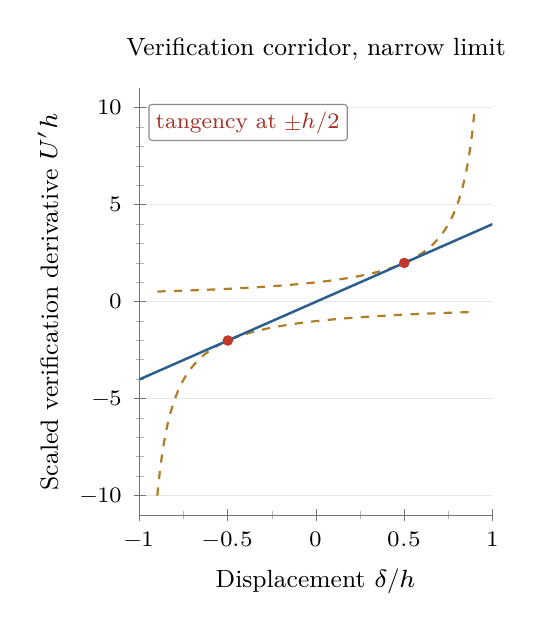
\begin{tikzpicture}
\begin{axis}[
  ltaxis,
  width=0.50\linewidth, height=7cm,
  xmin=-1, xmax=1, ymin=-11, ymax=11,
  xlabel={Displacement $\delta/h$},
  ylabel={Scaled verification derivative $U'h$},
  xtick={-1,-0.5,0,0.5,1}, ytick={-10,-5,0,5,10},
  minor x tick num=1, minor y tick num=4,
  title={Verification corridor, narrow limit},
  ymajorgrids,
]
\addplot[ltamber, line width=0.8pt, dashed, domain=-0.9:0.9, samples=120, forget plot]
  {1/(1-x)};
\addplot[ltamber, line width=0.8pt, dashed, domain=-0.9:0.9, samples=120, forget plot]
  {-1/(1+x)};
\addplot[ltblue, line width=0.9pt, domain=-1:1, samples=2, forget plot] {4*x};
\addplot[only marks, mark=*, mark size=1.7pt, ltred, forget plot]
  coordinates {(0.5,2) (-0.5,-2)};
\node[ltcallout, anchor=north west, text=ltred!85!black]
  at (axis cs:-0.95,10.2) {tangency at $\pm h/2$};
\end{axis}
\end{tikzpicture}\hfill
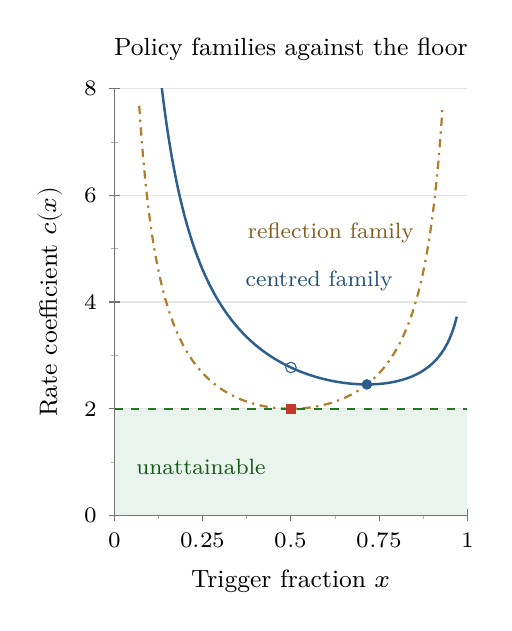
\begin{tikzpicture}
\begin{axis}[
  ltaxis,
  width=0.50\linewidth, height=7cm,
  xmin=0, xmax=1, ymin=0, ymax=8,
  xlabel={Trigger fraction $x$}, ylabel={Rate coefficient $c(x)$},
  xtick={0,0.25,0.5,0.75,1}, ytick={0,2,4,6,8},
  minor x tick num=1, minor y tick num=1,
  title={Policy families against the floor},
  ymajorgrids,
]
% nothing reaches below the floor
\path[fill=ltfloortint] (axis cs:0,0) rectangle (axis cs:1,2);
\addplot[ltblue, line width=0.9pt, domain=0.02:0.97, samples=150, forget plot]
  {-ln(1-x)/(x*x)};
\addplot[ltamber, line width=0.8pt, dash dot, domain=0.07:0.93, samples=150,
  forget plot] {1/(2*x*(1-x))};
\addplot[ltgreen!75!black, line width=0.8pt, dashed, domain=0:1, samples=2,
  forget plot] {2};
\node[font=\footnotesize, anchor=south west, text=ltgreen!55!black]
  at (axis cs:0.03,0.55) {unattainable};
\node[font=\footnotesize, anchor=east, text=ltamber!75!black]
  at (axis cs:0.88,5.30) {reflection family};
\node[font=\footnotesize, anchor=west, text=ltblue!85!black]
  at (axis cs:0.34,4.40) {centred family};
\addplot[only marks, mark=*, mark size=1.7pt, ltblue, forget plot]
  coordinates {(0.7153,2.4554)};
\addplot[only marks, mark=o, mark size=1.9pt, ltblue, forget plot]
  coordinates {(0.5,2.7726)};
\addplot[only marks, mark=square*, mark size=1.6pt, ltred, forget plot]
  coordinates {(0.5,2)};
\end{axis}
\end{tikzpicture}
\caption{Left, the narrow-limit corridor between the envelope slopes
(dashed) and the extremal verification derivative $4\delta/h^2$
(solid), tangent at $\pm h/2$. Right, the centred coefficient $c(x)$
(solid) and the reflection coefficient $c_{\mathrm{refl}}(x)$
(dash-dotted) against the floor at two, with the centred optimum
(filled), the production convention (open), and the reflection limit
sitting on the floor (square).}
\label{fig:corridor}
\end{figure}

% =========================================================================
\section{The width-uniform floor}\label{sec:width}

The second theorem removes the fixed-width hypothesis. Free moves
preserve $\omega_0$ at every width by Corollary~\ref{cor:free}, paid
moves are priced by Theorem~\ref{thm:share} at every width, and
between impulses the share diffuses with the price at a rate the
width controls. Write $\rho_W = W_{\max}/s_-$.

\begin{lemma}[Clock and Drift Bounds]\label{lem:clock}
Within a range $[a, b]$ of width $w = b - a$ containing the price,
$\phi(s, a, b) \le w$, and
\begin{equation}\label{eq:clock}
\omega_0'(s) \;=\; -\,\frac{(s - a)^2 + a\,(b - a)}{b\,\phi(s, a,
b)^2}, \qquad |\omega_0'| \;\ge\; \frac{a/b}{w}, \qquad
|\omega_0''| \;\le\; \frac{12\, b^2}{a^3\, w}.
\end{equation}
\end{lemma}

\begin{theorem}[Width-Uniform Floor]\label{thm:width}
Every $\mathcal{A}_2$ policy, variable in width and isolated, with
width cap $W_{\max}$ and $\rho_W \le 1/5$, satisfies
\begin{equation}\label{eq:widthfloor}
r \;\ge\; \frac{8\,\sigma_s^2}{W_{\max}^2}\,\big(1 - K_0
\rho_W\big) \;=\; \frac{2\,\sigma_s^2}{h_{\max}^2}\,\big(1 - K_0
\rho_W\big), \qquad h_{\max} = W_{\max}/2,
\end{equation}
with $K_0$ an absolute constant; $K_0 = 10$ suffices on the bounds of
Lemma~\ref{lem:clock} and is not optimised.
\end{theorem}

\begin{proof}[Proof sketch]
Run the verification argument on the state $\omega = \omega_0 \in
(0, 1)$ with $U(\omega) = 8(\omega - \tfrac12)^2$. The impulse
inequality is the corridor $-1/\omega \le U' \le 1/(1-\omega)$
against the share potentials of Theorem~\ref{thm:share}, with
tangency at $\omega = 1/4$ and $3/4$, the inequalities $(4\omega -
1)^2 \ge 0$ and $(4\omega - 3)^2 \ge 0$; this part is exact and
carries no narrow-limit correction at any width. The path of
$\omega$ is continuous across free impulses, its quadratic variation
is at least $(1 - \rho_W)^2 \sigma_s^2 / W_{\max}^2$ per unit
time by Lemma~\ref{lem:clock} and the cap, and its drift is
$O(\rho_W)$ against the clock term by the second-derivative
bound. Assembly in Appendix~\ref{app:floors}.
\end{proof}

\emph{In words, variable width buys nothing below the fixed-width
floor at the cap; small widths only speed the composition clock and
raise the bound, so no lower width bound is needed within the stated
era and cap regime.} The two ingredients are of different kinds. The
share corridor is exact at every width, being
Theorem~\ref{thm:share} itself, and the factor $1 - K_0 \rho_W$ is
entirely the cost of converting price variation into the share
clock. The consistency check is exact, since for fixed width the $\omega$-form reproduces
the $\delta$-form constant. The tangency constant is therefore not
an artefact of one coordinate; the same argument in the share
coordinate, tangent at $\omega = 1/4$ and $3/4$ rather than at $\pm
h/2$, returns the same two. The harness's widen-slide family, policies that widen
free towards the cap and pay only to slide back, never beats
\eqref{eq:widthfloor}, and its best member pays above the best
fixed-width-at-cap policy (Section~\ref{sec:verification}).

% =========================================================================
\section{The swap-mediated floor}\label{sec:swap}

Production operators do not surrender the mint surplus; they swap
first. The class $\mathcal{A}_1$ prices an impulse that moves the
holdings share from $\omega$ to $\omega'$ at
\begin{equation}\label{eq:swapcost}
k \;\ge\; \underbrace{\eta\,|\omega' - \omega|}_{\textnormal{fee}}
\;+\; \underbrace{I\,(\omega' - \omega)^2}_{\textnormal{impact}}
\;+\; \underbrace{\gamma}_{\textnormal{gas}},
\qquad I = \frac{V}{s L_p}, \quad
\gamma = \frac{G_{\mathrm{gas}}}{V},
\end{equation}
the three legs of Assumption~\ref{ass:execution} on the
notional $N_1$. Dust-mediated motion
costs at least one log-unit per unit of share by
Theorem~\ref{thm:share}, against the swap leg's fee scale, and
mixed moves price leg by leg, so \eqref{eq:swapcost} covers every
$\mathcal{A}_1$ impulse (Appendix~\ref{app:floors}).

\begin{theorem}[Swap-Mediated Floor]\label{thm:swap}
Every $\mathcal{A}_1$ policy at fixed width $w$ satisfies
\begin{equation}\label{eq:swapfloor}
r \;\ge\; A(\eta, \gamma, I)\;
\frac{(1 - \rho_w)^2\,\sigma_s^2}{w^2}, \qquad
\rho_w = \frac{w}{s_-}, \qquad
A \;=\; \min_{d \in (0, 1)} \frac{\gamma + \eta\,d +
I\,d^2}{d\,(1 - d)},
\end{equation}
The swap-mediated variable-width class, the join of $\mathcal{A}_1$
and $\mathcal{A}_2$, satisfies the same bound at $w = W_{\max}$. In the two tractable regimes,
\[
A = \eta \quad (\gamma = I = 0), \qquad
A = \eta + 2\sqrt{\gamma\eta} + O(\gamma) \quad
(I = 0,\ \gamma \ll \eta),
\]
the second with minimiser $d^* =
(\sqrt{\gamma^2 + \gamma\eta} - \gamma)/\eta$.
\end{theorem}

\begin{proposition}[Return-Point Achievability]\label{prop:return}
The renewal policy that fires at $|\delta| = x h$ and corrects back
by $m h$ on the same side pays
\begin{equation}\label{eq:rswap}
r(x, m) \;=\; \frac{\sigma_s^2}{h^2} \cdot
\frac{\eta\,m/2 + \gamma + I\,m^2/4}{m\,(2x - m)},
\end{equation}
decreasing in the trigger $x$, so the trigger optimum is the band
edge and the optimisation lives in the correction size $m$. In the
fee-only case, $r(1, m) \to \eta\,\sigma_s^2/w^2$ as $m \to 0$; the
sandwich of Theorem~\ref{thm:swap} is tight, with no gap. With gas
the optimal correction is $m^* \approx 2\sqrt{\gamma/\eta}$, the
Whalley--Wilmott scaling.
\end{proposition}

\emph{In words, with swaps, and on the execution objective alone,
the cheapest way to hold a band is to fire as late as possible and
correct as little as possible, and the cost of doing so approaches
fee times volatility squared over width squared, an infimum rather
than a rate any finite correction attains.} Edge-hugging is admissible here because the fee cost is
linear rather than logarithmic; the corner blow-up of
Remark~\ref{rem:corner} does not occur. It is a cost-side
idealisation, and Proposition~\ref{prop:cadence} and revenue
considerations move the practical optimum inward.

Three consequences follow. First, late firing, which
the population measurements of OF find implemented as dwell
and penetration rules, is cost-optimal in direction, there being no
interior trigger optimum from fee, impact,
and gas alone. Second, the deployed convention
(fire at $x = 0.5$, correct fully to centre) pays $(\eta +
4\gamma)\,\sigma_s^2/h^2$, between three and four times the floor
at production parameters. Table~\ref{tab:production} works the
numbers at the standing production anchors, price volatility
$80\,\%$ per square-root year so $\sigma_s/\bar s = 0.40$, $\rho =
0.02$, $\eta = 10^{-4}$, gas $\$0.03$ per event. Third, the floor
is a benchmark. For a position of width $w$, realised fractional
dissipation per unit time (fees plus gas plus impact plus residual
dust, over mean value) divided by $A\,(1-\rho_w)^2
\hat\sigma_s^2/w^2$ is a dimensionless score with the floor at one;
the score prices the correction-size and width choices, and does not
price the trigger, whose late-firing direction is already optimal.
The isolated-class optimum $x^* = 0.7153$ of
Proposition~\ref{prop:achieve} is not the reference for any
swap-mediated operator.

\begin{table}[H]
\centering
\caption{The swap-mediated floor at production anchors.}
\label{tab:production}
\begin{tabular}{@{}lccc@{}}
\toprule
 & $V = \$10$k & $V = \$100$k & $V = \$1$M \\
\midrule
$\gamma = G_{\mathrm{gas}}/V$ & $3.0\times10^{-6}$ & $3.0\times10^{-7}$ & $3.0\times10^{-8}$ \\
$d^*$ & $0.146$ & $0.052$ & $0.017$ \\
$A$ & $1.41\times10^{-4}$ & $1.12\times10^{-4}$ & $1.04\times10^{-4}$ \\
floor $A\,\sigma_s^2/w^2$ & $1.41\,\%/\mathrm{yr}$ & $1.12\,\%/\mathrm{yr}$ & $1.04\,\%/\mathrm{yr}$ \\
deployed convention & $4.5\,\%/\mathrm{yr}$ & $4.05\,\%/\mathrm{yr}$ & $4.0\,\%/\mathrm{yr}$ \\
\bottomrule
\end{tabular}
\end{table}

% =========================================================================
\section{The retention collapse}\label{sec:collapse}

The floors so far assume the surplus is lost. The last theorem-grade
statement concerns the architecture that keeps it. In
$\mathcal{A}_3$ the state carries standing balances
$(x_{\mathrm{d}}, y_{\mathrm{d}})$; an impulse mints from $\hat x =
x_w + x_{\mathrm{d}} - x_{\mathrm{sw}}$ and $\hat y = y_w + y_{\mathrm{d}}
- y_{\mathrm{sw}}$ through the same binding-side minimum, and the surplus
is credited back to the balances rather than emitted, the
ledger-inclusive mint identity established in ME.\cite{ryan2026master} Define
the system value $V_{\mathrm{sys}} = V + V_{\mathrm{d}}$, position
plus ledger, with the ledger valued at the impulse price.

\begin{proposition}[Retention Collapse]\label{prop:collapse}
In $\mathcal{A}_3$, the impulse being atomic so that withdrawal and
re-mint price at one $s$, $V_{\mathrm{sys}}$ is conserved at every
swap-free impulse, and at a swap-corrected impulse its loss is the
swap's fee, impact, and gas under
Assumption~\ref{ass:execution}. The impulse leg of the
dissipation functional on $V_{\mathrm{sys}}$ therefore carries no
term of order $\sigma_s^2/h^2$ or $\eta\,\sigma_s^2/w^2$; the floors
of Theorems~\ref{thm:fixed}, \ref{thm:width}, and~\ref{thm:swap} are
deleted, not lowered.
\end{proposition}

\begin{proof}
Token conservation at the impulse is the arithmetic of ME's jump
theorem, whose credited balances sum with the mint's consumption to
the available amounts token by token; valuing both sides at the
impulse price gives value conservation, and the swap legs are priced
as in \eqref{eq:swapcost}. No verification function is needed.
\end{proof}

\emph{In words, an architecture that keeps the residuals inside the
system carries no emission term in the impulse leg of its system
value, only the execution costs of its corrective swaps; the floor
is a property of emission, and retention deletes it from that leg
rather than lowering it. The concavity leg and the exposure of the
retained inventory are untouched.} The emission precondition is the one GS
established with a stock-manager fork test and ME formalised, and
the concurrent topology preprint\cite{pi2026convexity} gives
the multi-pool circulation condition for it. Three residual costs
survive retention. The
ledger is idle inventory with one-sided price exposure, an
opportunity cost the functional does not price; forcing its
redeployment through swaps pays the $\mathcal{A}_1$ fee scale on the
recycled flux; and the concavity leg is untouched by architecture.
For the Siphonic design, retention collapses the rebalancing
dissipation floor to fees, gas, and execution impact.

% =========================================================================
\section{The menu and the cadence term}\label{sec:menu}

The floors take the venue's rounding rule and the operator's
monitoring as given. Two propositions price them as additive terms,
the first designer-facing, the second operator-facing. Both consume
the offset and monitoring machinery of Sections~\ref{sec:lemma}
and~\ref{sec:extensions}.

\begin{proposition}[Quantisation Menu]\label{prop:menu}
Let the impulse map centre ranges on a grid of spacing $\vartheta$
and size at the floor tick, and let the firing-state offset be
uniform to the error of Lemma~\ref{lem:conditional}. Then the rate carries two
additive terms conditional on the deployed rule.
\begin{enumerate}[label=(\roman*)]
\item \emph{Placement.} The re-placement lands off-centre by the
placement offset $o \in [0, \vartheta)$, so the rate is the renewal
family's at $\delta_0 = o$ averaged over the offset law; at the
family optimum the penalty is second-order in $\vartheta$, and at a
deployed non-optimal configuration it carries the first-order term
$\partial r/\partial \delta_0 \cdot \vartheta/2$, signed by the
one-sidedness of the floor.
\item \emph{Sizing.} Floor-tick sizing adds the per-event expected
fraction $g\,\mathbb{E}|\zeta + \Delta|$ of OQM's value channel,
a rate term $\lambda\, g\,\mathbb{E}|\zeta + \Delta|$; nearest-tick
sizing halves the offset contribution and continuous-price sizing
deletes it.
\end{enumerate}
\end{proposition}

\emph{In words, where the range is allowed to land and how its size
is rounded are two priced lines of the rate, and each deployed rule
carries its own per-event price, additive at the offset and renewal
conditions of the proposition.} Rounding is thereby a policy
instrument.

\begin{proposition}[Cadence Term]\label{prop:cadence}
For an operator whose trigger sits at displacement $xh$, firing at
the first check after the crossing, with
check interval $\Delta t$, the firing displacement carries the
flat-entry overshoot with mean $\sqrt{2\pi}\,\sigma_1/4 \approx
0.63\,\sigma_1$ of Proposition~\ref{prop:monitoring}(i), and to
leading order the rate gains the additive term
\[
\lambda\,\big[\,k'(xh)\,\mathbb{E}[O]
- k(xh)\,\Theta\,\big],
\]
the
overshoot priced along the envelope slope against the cadence
thinning credit $\Theta$ of the barrier-shift correction; the first
term dominates in the isolated class and the two are comparable in
the swap class.
\end{proposition}

\emph{In words, an operator who checks every $\Delta t$ pays for the
displacement the price builds past the line between checks, less a
small credit from the crossings the gap lets escape.}
The population measurements of OF find most production firing
gated by dwell and penetration rules rather than cadence, with
overshoot roughly invariant in actuation delay, which is a chosen
trigger shift rather than a monitoring cost. A deterministic
penetration threshold re-parametrises the trigger, which
Proposition~\ref{prop:return} makes cheaper per event in the swap
class, and whose benefit is the avoided round-trip cost of
whipsawed firings, both potential increments of
Corollary~\ref{cor:family}. Pricing that trade in full requires the
out-of-range leg of the dissipation identity and is left to future
work on the churn accounting.

% =========================================================================

% =========================================================================
\section{The two legs compared}\label{sec:legscompared}

The comparison between the two legs
reverses across architectures, which refines the additivity
reading of OQM.

\begin{proposition}[Leg Comparison]\label{prop:legs}
For a centred narrow range the concavity leg runs at fractional rate
approximately $\sigma_s^2/(2 \bar s h)$. The isolated-class floor
exceeds it by the factor $4/\rho$ at the floor constant, two orders
of magnitude at production concentration, while the swap-mediated
floor is smaller than it by approximately $\eta/(2\rho)$, roughly
$1/400$ at the production anchors.
\end{proposition}

\emph{In words, in the isolated architecture the event leg is
parametrically the leading cost, while for swap-mediated operators the event floor is a small
correction to the concavity cost, which is why the floor is a
benchmark rather than a headline expense.}
The reversal is the practical content of the architecture choice;
an isolated venue's operators face the event leg as their dominant
cost, a swap venue's operators face it as a controllable
correction, and only retention removes it from the ledger
altogether (Section~\ref{sec:collapse}).


\actdivider{Act III}{The Instrument}

\noindent\emph{The third act inverts the law. A deployed trigger
line is a threshold detector for the price process, and the
population's firing records are read, through the jump and
monitoring layers of Section~\ref{sec:extensions}, for the
diffusive scale and the integrated jump tails the operators
themselves face; the naive reading fails, and the
conditioned reading is the instrument, and it is conditional
throughout, on the geometry census, the era, the monitoring
admissions, and the discreteness cut. Notation is the first act's;
Appendix~\ref{app:glossary} collects it.}

% =========================================================================
\section{The instrument}\label{sec:instrument}

The third act derives a conditional inverse map from the firing
records of the deployed population to the jump part of the
dissipation measure's impulse component
(Definition~\ref{def:ximeasure}). What it identifies is a family of
integrated jump-tail functionals per pool, under the geometry, era,
monitoring, and discreteness admissions, and not the jump measure
itself.

\subsection{Price, detectors, observables}\label{sec:observables}

Within an era the price coordinate follows
\begin{equation}\label{eq:eramodel}
X_t \;=\; x_0 + \mu t + \sigma B_t + X^J_t,
\end{equation}
with $B$ standard Brownian motion and $X^J$ a pure-jump part whose
compensator is time-homogeneous per era, $\nu^X(dt, dz) = dt\,
\nu(dz)$, with $\int (|z| \wedge 1)\, \nu(dz) < \infty$. Hypothesis
(F5) below adds first-moment integrability where the tail
functionals require it. Eras are the stationarity windows of the
population work of OF; every statement in this paper is per
era.

An operator holds a trigger line at $b$ (the up-crossing side is
treated throughout; the down side is symmetric), monitors at check
times $(t_j)$ with intensity $\chi_t$, deterministic cadence
$\Delta t$, Poisson, and Cox-type checking all admitted, and fires at
the first check at which its firing condition holds. The policy
filter is the pair $(p_{\mathrm{pen}}, d_{\mathrm{dw}})$, a
penetration threshold and a dwell requirement, era-constant per
operator; the plain threshold policy is $(0, 0)$. Per firing event
the observables are the overshoot $O = X_{\tau_f} - b$
and the actuation delay $\tact = \tau_f - \tau_c$,
where $\tau_c$ is the most recent entry time of the price into
$\{x \ge b\}$ before the firing. This is what the data supply. The
line $b$ is recovered per operator from the firing-position
discontinuity,\cite{ryan2026fingerprint} and $\tau_c$ is measured on the
pool's public tick stream by walking back from the firing block to
the last inside-to-outside transition. The detector is not the
analyst's construction; its line, its cadence and its filter are
read from deployed code and the record that code leaves.

Crossings split by type, following the firing split $N =
N^{c} + N^{J}$ of the
jump-crossing compensator of Appendix~\ref{app:intensity}. The
split is at the level of the compensator, and no event in the data
carries its type as a label. A continuous
crossing has $X_{\tau_c} = b$. A jump crossing has $X_{\tau_c-} = b -
Y < b$ and $X_{\tau_c} = b - Y + z$ for a jump of size $z > Y$, and
the straddle depth is $O_J = z - Y > 0$, latent at every event and
reached only through the overshoot law. The observability remark of
Section~\ref{sec:jumps}, that the overshoot at a jump firing is
bounded below by the straddle depth, becomes an exact per-event law
below and is then inverted. Figure~\ref{fig:spectrometer} draws the
two crossing types.

\begin{figure}[H]
\centering
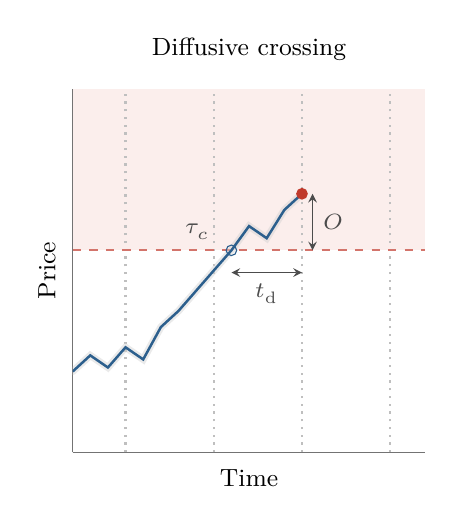
\begin{tikzpicture}
\begin{axis}[
  ltaxis,
  width=0.50\linewidth, height=6.2cm,
  xmin=0, xmax=1, ymin=0.1, ymax=1,
  xlabel={Time}, ylabel={Price},
  xtick=\empty, ytick=\empty,
  title={Diffusive crossing},
]
% outside the trigger
\path[fill=ltalerttint] (axis cs:0,0.60) rectangle (axis cs:1,1);
% check times
\foreach \c in {0.15, 0.40, 0.65, 0.90}
  \addplot[black!25, dotted, thick, forget plot]
    coordinates {(\c,0.1) (\c,1)};
% trigger line b
\addplot[ltred!70, thick, dashed, domain=0:1, samples=2, forget plot] {0.60};
% path
\addplot[ltblue, line width=0.9pt, ltglow, forget plot] coordinates {
(0.0,0.30) (0.05,0.34) (0.10,0.31) (0.15,0.36) (0.20,0.33)
(0.25,0.41) (0.30,0.45) (0.35,0.50) (0.40,0.55) (0.45,0.60)
(0.50,0.66) (0.55,0.63) (0.60,0.70) (0.65,0.74)
};
% crossing and firing marks
\addplot[only marks, mark=o, mark size=1.9pt, ltblue, forget plot]
  coordinates {(0.45,0.60)};
\addplot[only marks, mark=*, mark size=1.9pt, ltred, forget plot]
  coordinates {(0.65,0.74)};
% overshoot O
\draw[black!70, <->, >=stealth] (axis cs:0.68,0.60) --
  (axis cs:0.68,0.74) node[midway, right, font=\footnotesize] {$O$};
% delay
\draw[black!70, <->, >=stealth] (axis cs:0.45,0.545) --
  (axis cs:0.65,0.545) node[midway, below, font=\footnotesize] {$\tact$};
\node[font=\footnotesize, anchor=south east, black!70] at
  (axis cs:0.42,0.60) {$\tau_c$};
\end{axis}
\end{tikzpicture}\hfill
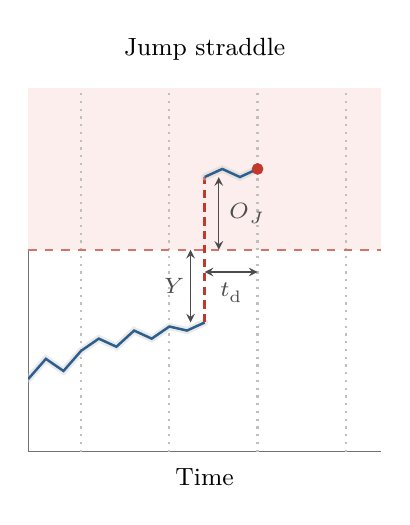
\begin{tikzpicture}
\begin{axis}[
  ltaxis,
  width=0.50\linewidth, height=6.2cm,
  xmin=0, xmax=1, ymin=0.1, ymax=1,
  xlabel={Time},
  xtick=\empty, ytick=\empty,
  title={Jump straddle},
]
\path[fill=ltalerttint] (axis cs:0,0.60) rectangle (axis cs:1,1);
\foreach \c in {0.15, 0.40, 0.65, 0.90}
  \addplot[black!25, dotted, thick, forget plot]
    coordinates {(\c,0.1) (\c,1)};
\addplot[ltred!70, thick, dashed, domain=0:1, samples=2, forget plot] {0.60};
% pre-jump path below the line
\addplot[ltblue, line width=0.9pt, ltglow, forget plot] coordinates {
(0.0,0.28) (0.05,0.33) (0.10,0.30) (0.15,0.35) (0.20,0.38)
(0.25,0.36) (0.30,0.40) (0.35,0.38) (0.40,0.41) (0.45,0.40)
(0.50,0.42)
};
% the jump
\addplot[ltred, line width=1.0pt, densely dashed, forget plot]
  coordinates {(0.50,0.42) (0.50,0.78)};
% post-jump path to firing
\addplot[ltblue, line width=0.9pt, ltglow, forget plot] coordinates {
(0.50,0.78) (0.55,0.80) (0.60,0.78) (0.65,0.80)
};
\addplot[only marks, mark=*, mark size=1.9pt, ltred, forget plot]
  coordinates {(0.65,0.80)};
% pre-jump gap Y and straddle depth O_J
\draw[black!70, <->, >=stealth] (axis cs:0.46,0.42) --
  (axis cs:0.46,0.60) node[midway, left, font=\footnotesize] {$Y$};
\draw[black!70, <->, >=stealth] (axis cs:0.54,0.60) --
  (axis cs:0.54,0.78) node[midway, right, font=\footnotesize] {$O_J$};
\draw[black!70, <->, >=stealth] (axis cs:0.50,0.545) --
  (axis cs:0.65,0.545) node[midway, below, font=\footnotesize] {$\tact$};
\end{axis}
\end{tikzpicture}
\caption{The two crossing types read by the instrument, with check
times dotted, the trigger $b$ dashed, and the region beyond it
tinted. Left, a diffusive crossing at $\tau_c$ (open) fires at the
next admitted check (filled) with monitoring overshoot $O$; right, a
jump from gap $Y$ below the line lands $O_J$ beyond it, and the
firing overshoot is bounded below by that straddle depth.}
\label{fig:spectrometer}
\end{figure}

\subsection{Hypotheses}\label{sec:hypotheses}

Six hypotheses carry the theory;
Table~\ref{tab:hypotheses} states each beside the measurement that
certifies it. Certification here means that the hypothesis's
designed check passes at its stated power, reported where each
check runs; it is measured consistency, not proof. The exclusion restriction (F4) says that checking
responds to activity, not to the size of the individual jump; (F5)
is the one purely assumed member, a moment hypothesis the tail
functionals consume.

\begin{table}[H]
\centering
\caption{The instrument's hypotheses and their certifications.}
\label{tab:hypotheses}
{\footnotesize
\begin{tabular}{@{}lp{0.46\linewidth}p{0.34\linewidth}@{}}
\toprule
 & Hypothesis & Certified by \\
\midrule
(F1) & era homogeneity; the parameters of \eqref{eq:eramodel} and the policy filters constant per era & era-half replication, binding per pool (Section~\ref{sec:certifications}) \\
(F2) & flat entry at the one-check scale near the line; flat gap occupation where the jump tail varies, the exact kernel available where flatness fails & drift and leakage bound, budget row 1; kernel form of Lemma~\ref{lem:straddle} \\
(F3) & policy filter era-constant per operator & within-pool agreement design (Section~\ref{sec:agreement}) \\
(F4) & given a jump crossing and the volatility state, check intensity independent of the straddle depth & exceedance shape across cadence strata (Section~\ref{sec:certifications}) \\
(F5) & $m_1 = \int z^{+}\, \nu(dz) < \infty$ & moment hypothesis, not separately tested \\
(F6) & crossing time measured with bounded staleness & dense-crossing admission, budget row 4 \\
\bottomrule
\end{tabular}}
\end{table}

% =========================================================================
\section{The forward map}\label{sec:forward}

\subsection{The diffusive branch}\label{sec:diffusive}

The monitoring kernel and the delay law follow from the flat-entry
hypothesis exactly as in Appendix~\ref{app:intensity}, but resolved
in the delay variable rather than marginalised over it.

\begin{lemma}[Conditional Kernel]\label{lem:kernel}
Under the plain threshold policy, conditional on a continuous
crossing at $\tau_c$ and firing at the
next check, at delay $\tact = a$, the overshoot has the folded
normal density at scale $\sigma\sqrt{a}$,
\[
g_{O \mid a}(o) \;=\; \frac{2}{\sigma\sqrt{a}}\,
\nden\big(o/\sigma\sqrt{a}\big), \qquad o > 0,
\]
and the per-check qualification probability given $a$ is $1/2$,
independent of $a$. Penetration and dwell filters change that
probability and enter through the policy filter of
Section~\ref{sec:policy}.
\end{lemma}

\begin{lemma}[Flat-Entry Delay Law]\label{lem:delay}
Under flat entry, conditional on firing at a check, the
crossing-to-check delay has density
\[
g_{\mathrm{act}}(a) \;=\; \frac{1}{2\sqrt{\Delta t}\,
\sqrt{\Delta t - a}}, \qquad a \in (0, \Delta t),
\]
increasing towards $a = \Delta t$, so observed delays are long. The
two readings are one fact, crossings clustering early in the check
interval because states arbitrarily close to the line cross
immediately.
\end{lemma}

\begin{proposition}[Exact Reproduction]\label{prop:reproduction}
The $a$-marginal of the joint law of
Lemmas~\ref{lem:kernel}--\ref{lem:delay} is exactly the
flat-entry overshoot density of Proposition~\ref{prop:monitoring}(i),
\[
\int_0^{\Delta t} g_{\mathrm{act}}(a)\, g_{O\mid a}(o)\, da
\;=\; \frac{\sqrt{2\pi}}{\sigma_1}\, \surv(o/\sigma_1).
\]
\end{proposition}

\emph{In words, resolving the overshoot by delay and then averaging
over the delay law returns exactly the overshoot density the
monitoring layer promised, so the delay-resolved instrument and the
marginal law are one construction.}

The proof (Appendix~\ref{app:proofs}) reduces the integral, after
normalising to unit scale, by the substitution $a = 1/(1 + s^2)$ to
the integrand of Owen's $T$,\cite{owen1956} then evaluates it by an
inner antiderivative and an interchange rather than by quoting the
special function's limit value. That evaluation is machine-checked
in the formalisation. The substitution is improper at both endpoints
and is not, so the harness's fifteen-digit assertion of the
assembled identity now covers that step alone. Three corrections are
carried rather than re-derived; drift shifts the kernel mean by $\mu
a = o(\sigma\sqrt{a})$ under flat entry, sequential conditioning on
earlier failed checks is the barrier-shift correction of Broadie,
Glasserman, and Kou\cite{bgk1997} at leading order, and Poisson or
Cox checking replaces Lemma~\ref{lem:delay} by the first-check law
of the $\chi$ process after $\tau_c$ while Lemma~\ref{lem:kernel} is
untouched, since it conditions only on the delay's value.

\subsection{The jump branch}\label{sec:jumpbranch}

\begin{lemma}[Straddle Law]\label{lem:straddle}
On jump crossings, with $\psi_b(y)$, $y > 0$, the occupation density
of the pre-jump gap $Y = b - X_{\tau_c-}$ over the excursion
preceding the crossing, normalised to a probability density in $y$,
\[
\mathbb{P}(O_J > o) \;=\;
\frac{\int_0^\infty \psi_b(y)\, \bar\nu(y + o)\, dy}
{\int_0^\infty \psi_b(y)\, \bar\nu(y)\, dy},
\qquad
\lambda_J \;=\; \int_0^\infty \psi_b(y)\, \bar\nu(y)\, dy,
\]
where $\bar\nu(y) = \nu((y, \infty))$ and $\lambda_J$ is the
occupation-averaged jump-crossing intensity, per unit time under
that normalisation, which is also the normalisation
Proposition~\ref{prop:multiscale} compares across operators. If $\psi_b$ is flat at
the scale where $\bar\nu$ varies and $m_1 = \int_0^\infty
\bar\nu(z)\, dz < \infty$, the straddle depth has density and
survival
\[
g_J(o) \;=\; \frac{\bar\nu(o)}{m_1}, \qquad
\mathbb{P}(O_J > o) \;=\; \frac{\jtail(o)}{\jtail(0)}, \qquad
\jtail(o) := \int_o^\infty \bar\nu(z)\, dz .
\]
\end{lemma}

This is the ladder-height structure of renewal
theory\cite{asmussen2003} inherited through the occupation measure
rather than through renewal cycles. The flat form is the
leading-order reading; the exact kernel form is what the multiscale
theorem uses, since $\psi_b$ is estimable per cell from the tick
stream and the recovered placement, and the tail exponent survives
any integrable $\psi_b$ because $\int \psi_b(y)\, \bar\nu(y + o)\,
dy \sim \bar\nu(o) \int \psi_b$ as $o \to \infty$ under regular
variation.

\begin{lemma}[Post-Crossing Composition]\label{lem:composition}
Conditional on a jump crossing with straddle depth $o_J$ and firing
at delay $a$, the overshoot is $O = o_J + \mu a + \sigma\sqrt{a}\,
Z_a$ with $Z_a$ the post-crossing displacement normalised to unit
scale, conditioned on the policy filter's qualification event; for
the plain threshold policy and $o_J \gg \sigma\sqrt{a}$ the
conditioning is negligible and $Z_a$ is standard normal. The straddle
component stays at $o_J$ whatever the delay, while the post-crossing
motion contributes the drift $\mu a$ and a monitoring component of
order $\sigma\sqrt{a}$.
\end{lemma}

\subsection{The policy filter}\label{sec:policy}

Policy filters decide which crossings reach the record, and they
leave two signatures at opposite ends of the delay axis. At long
delay a dwell or penetration rule holds the overshoot at its own
scale, which is the filter's signature; at small delay the same rule
suppresses the diffusive branch far faster than the jump branch,
which is the signature the identification uses.

\begin{lemma}[Delay Invariance]\label{lem:invariance}
Consider an era-constant dwell or penetration policy on an ergodic
era model, and assume the excursion above the line, conditioned on
survival, converges past a relaxation time to a quasi-stationary
law with finite second moment. Then the conditional law of $O$
given $\tact = a$ converges as $a \to \infty$ to an
operator-specific limit that does not depend on $a$, so
$\mathbb{E}[O^2 \mid \tact = a]/(\sigma^2 a) \to 0$; the pure-lag
alternative, firing at the first sparse check with no filter, gives
$\mathbb{E}[O^2 \mid \tact = a] \asymp \sigma^2 a$ with no
hypothesis beyond the era model.
\end{lemma}

The dichotomy is the discriminating measurement between policy and
plumbing, and the population data fall on the policy side
(Section~\ref{sec:evidence}). At population level the invariance
appears as clustering, each operator's events concentrated near its
own filter scale, so the cross-population scan mixes operator
clusters; the per-operator scan needs the penetration form, whose
attainment time spreads the delay axis, a point the synthetic
harness makes exact.

\begin{lemma}[Jump Enrichment]\label{lem:enrichment}
Under a penetration filter $p_{\mathrm{pen}} > 0$, the continuous
branch's probability of firing within delay $a$ of its crossing is
$O\big(\exp(-p_{\mathrm{pen}}^2/2\sigma^2 a)\big)$, while the jump
branch's is bounded below by $\mathbb{P}(O_J >
p_{\mathrm{pen}})\,\mathbb{P}(\text{check within } a)$, linear in
the check intensity. Dwell gates both branches equally. Among
operators whose filter is penetration-dominated, conditioning on
small $\tact$ therefore enriches the jump share beyond the
unconditional rate ratio $\lambda_J/(\lambda_J +
\lambda_c)$.
\end{lemma}

\subsection{The instrument response}\label{sec:response}

\begin{proposition}[Instrument Response]\label{prop:mixture}
Under (F1)--(F6), the joint law of overshoot and actuation delay at
a firing of an operator with policy filter $(p_{\mathrm{pen}},
d_{\mathrm{dw}})$, era parameters $(\mu, \sigma, \nu)$, and check
intensity $\chi$ is the two-branch mixture
\[
\mathbb{P}(O \in do,\; \tact \in da)
\;=\; \underbrace{\pi_c\, \Pi_c(da)\; K\big(do \mid a;\,
0\big)}_{\textnormal{diffusive branch}}
\;+\; \underbrace{\pi_J\, \Pi_J(da) \int_0^\infty g_J(o_J)\,
K\big(do \mid a;\, o_J\big)\, do_J}_{\textnormal{jump branch}},
\]
where $\pi_c, \pi_J$ are the check-weighted crossing-type shares,
$\Pi_c, \Pi_J$ are the crossing-type delay laws
(Lemma~\ref{lem:delay} in the deterministic-cadence flat-entry
specialisation; the $\chi$ first-arrival law thinned by
qualification in general; both supported on $a \ge d_{\mathrm{dw}}$
under dwell), and $K(\cdot \mid a; o_J)$ is the law of $o_J + \mu a
+ \sigma\sqrt{a}\, Z_a$ conditioned on qualification past $b +
p_{\mathrm{pen}}$ per Lemmas~\ref{lem:kernel}
and~\ref{lem:composition}, with $g_J$ as in
Lemma~\ref{lem:straddle}.
\end{proposition}

\emph{In words, every crossing-triggered firing of an admitted
operator is a draw from a two-branch mixture, a
diffusive branch whose overshoot shrinks with the actuation delay
and a jump branch whose overshoot does not, weighted by how the
checks land on the two crossing types.}

Three specialisations recover known statements. Setting $\nu = 0$
with the plain filter and deterministic cadence collapses to
Proposition~\ref{prop:monitoring}(i) exactly
(Proposition~\ref{prop:reproduction}); $a \to \infty$ under a
filter gives the delay-invariant policy plateau
(Lemma~\ref{lem:invariance}); and $a \to 0$ suppresses the first
branch at rate $\sqrt{a}$, faster under penetration
(Lemma~\ref{lem:enrichment}), leaving $g_J$ convolved with an
$O(\sigma\sqrt{a})$ kernel, which is the identification limit.

Check-intensity dependence is carried, not assumed away. If keepers
densify checks in volatile windows and jumps cluster with
volatility, the jump branch's delay law is stochastically smaller
than the continuous branch's, and the crossing-type shares are
check-weighted rather than time-averaged. Under (F4) the
conditional law of $O_J$ given a jump crossing and a delay value
does not depend on $\chi$, so every tail-shape functional read from
the small-delay subsample is clean; what $\chi$ contaminates is the
level, the conversion of shares into absolute rates, which is
identified relative to the continuous rate or jointly with a
recovered cadence. The harness verifies both halves of this split.


% =========================================================================
\section{Identification}\label{sec:ident}

Fix a pool-era with local diffusive scale $\sigma$. The target
functionals are the integrated tails $\jtail$ of
Lemma~\ref{lem:straddle}, whose normalised version is the straddle
survival, together with the per-geometry
jump-crossing rates. Define, for a multiplier $\kappa > 0$ and delay
cut $\bar a$, the exceedance functional
\[
\mathcal{E}(\kappa, \bar a) \;=\; \mathbb{P}\big(O > \kappa\,
\sigma \sqrt{\tact}\;\big|\; 0 < \tact \le \bar a\big),
\]
and write $\pi_J(\bar a)$ for the jump-crossing share of firings
with $\tact \le \bar a$.

\begin{theorem}[Small-Delay Identification]\label{thm:smalldelay}
Under (F1)--(F6), for every $\kappa \ge 1$ and $\bar a$ with
$|\mu| \bar a \le \tfrac12 \kappa\sigma\sqrt{\bar a}$,
\[
\big|\, \mathcal{E}(\kappa, \bar a) - \pi_J(\bar a)\, \big| \;\le\;
\underbrace{2\,\surv(\kappa/2)}_{\textnormal{diffusive leakage}}
\;+\; \underbrace{\pi_J(\bar a)\,
\Big(1 - \frac{\jtail(2\kappa\sigma\sqrt{\bar a})}{\jtail(0)}\Big)
}_{\textnormal{resolution floor}}
\;+\; \underbrace{\varepsilon_{\mathrm{cens}}}_{\textnormal{staleness}},
\]
rows 1, 2, and 4 of the bias budget (Table~\ref{tab:budget}),
with $\varepsilon_{\mathrm{cens}}$ the one-sided crossing-staleness error
controlled by the dense-crossing admission (F6). In particular
$\mathcal{E} \to \pi_J(0^+)$ as $\bar a \to 0$ with $\kappa \to
\infty$ and $\kappa\sqrt{\bar a} \to 0$, and the excess of $\mathcal{E}$ over
the folded normal baseline $2\surv(\kappa)$ is a consistent reading
of the small-delay jump share.
\end{theorem}

\emph{In words, at small actuation delay the diffusive branch cannot
manufacture large overshoots, so the rate of exceedances beyond a
few local scales reads the jump share directly, with a three-term
error the design controls.}

\begin{corollary}[Tail Shape]\label{cor:tailshape}
With $o_{\min} = \kappa\sigma\sqrt{\bar a}$, for every $o \ge 2
o_{\min}$,
\[
\mathbb{P}\big(O > o \;\big|\; \tact \le \bar a,\; O > o_{\min}\big)
\;=\; \frac{\jtail(o)}{\jtail(o_{\min})}
\Big(1 + O\big(\sigma\sqrt{\bar a}\,
\|g_J\|_{\mathrm{Lip}} \cdot \jtail(0)/\jtail(o_{\min})\big)
+ O\big(\surv(\kappa/2)/\mathcal{E}\big)\Big),
\]
so the normalised integrated tail is identified on $[o_{\min},
\infty)$, the resolution floor shrinking as $\sqrt{\bar a}$; under
the exact kernel form of Lemma~\ref{lem:straddle} the identified
object is the $\psi_b$-weighted analogue, with $\psi_b$ estimated
rather than assumed.
\end{corollary}

\emph{In words, above a resolution floor that shrinks with the check
interval, the shape of the observed overshoot tail is the shape of
the integrated jump tail.}

\begin{proposition}[Multiscale Identification]\label{prop:multiscale}
Let one pool-era host operators $i = 1, \dots, k$ with
certified-distinct geometries, recovered line distances and
estimated gap-occupation kernels $\psi_i$, so that operator $i$'s
jump-crossing rate is $\lambda_J^{(i)} = \int \psi_i(y)\,
\bar\nu(y)\, dy$. Then (i) each $\lambda_J^{(i)}$ is identified from
operator $i$'s firing record by Theorem~\ref{thm:smalldelay} and the
relative-rate conversion; (ii) if $\bar\nu$ and the $\psi_i$ lie in $L^2(0, \infty)$, the
vector $(\lambda_J^{(1)}, \dots,
\lambda_J^{(k)})$ identifies the orthogonal projection of $\bar\nu$
onto $\mathrm{span}\{\psi_i\}$ in that space if and only if the Gram
matrix $\int \psi_i \psi_j$ is nonsingular, a condition computable from the
estimated kernels; (iii) if $\bar\nu$ is regularly varying with
index $-\alpha$, $\alpha > 1$, and two kernel scales $s_1 < s_2$ are
separated, then $\lambda_J^{(2)}/\lambda_J^{(1)} =
(s_2/s_1)^{-\alpha}(1 + O(\varepsilon_{\mathrm{ker}}))$, so $k \ge
2$ separated geometries identify the index $\alpha$. The amplitude
follows only under a stated power-law convention $\bar\nu(y) \simeq
C\,y^{-\alpha}$, regular variation fixing the ratio and not the
constant. Precision degrades as $s_2/s_1 \to 1$, with
$\varepsilon_{\mathrm{ker}}$ bounded by the certified kernel
deviation.
\end{proposition}

\emph{In words, one operator identifies its pool's integrated jump
tail, operators at separated trigger scales identify the tail's
index, and the geometry census decides pool by pool which reading is
available.}

The proposition is conditional on the per-pool geometry count, whose
measured distribution is reported as data in
Section~\ref{sec:evidence}. The single-operator tail shape
(Corollary~\ref{cor:tailshape}) and the cross-operator rate ratios
(Proposition~\ref{prop:multiscale}(iii)) estimate the same index, which
supplies an overidentification check wherever a pool hosts both a
fast operator and a spread of geometries.

\begin{proposition}[Diffusive Corollary]\label{prop:diffusive}
At $\nu = 0$ the instrument degenerates to a volatility sensor; the
intensity representation of Proposition~\ref{prop:intensity}
recovers $\sigma^2$
per cell up to the operator's filter thinning, so population firing
rates estimate diffusive variance after per-sensor calibration, and
aggregation across sensors requires precision weighting rather than
averaging.
\end{proposition}

\emph{In words, with no jumps the population of detectors is a
volatility sensor, and each sensor is calibrated through its own
filter before any aggregation.} The proposition folds the
volatility-oracle reading into
the paper as the zeroth-order inversion; its content at $\nu \ne 0$
is that the same calibration discipline governs the jump reading,
which is why the estimators below never pool across pools.

% =========================================================================
\section{Estimators and the bias budget}\label{sec:estimators}

\subsection{Definitions}\label{sec:defs}

All estimators operate per pool-era; their full definitions,
admission thresholds, and interval mechanics are collected in
Appendix~\ref{app:estimators}. The local scale is a trailing
bipower estimate over $H$ blocks ending strictly before the
crossing block, so the candidate displacement is excluded; the
realised-variance variant is reported alongside, and its inflation
is a bias-budget row. The per-pool readings of
Section~\ref{sec:evidence} are captured with the realised-variance
variant of the trailing scale; row 3 of the budget signs the
difference, so the quoted excesses are conservative
(Section~\ref{sec:certifications}). Per admitted event the
overshoot is scored in trailing local scales, and the per-pool
exceedance fraction beyond the cut $\kappa = 3$ carries a Wilson
interval,\cite{wilson1927} with the jump share $\hat\pi_J$ read off
by subtracting the folded-normal baseline and the tail functional
taken as the empirical survival of exceedance sizes above
$o_{\min}$. Within a pool, strata combine by event count, the
precision weights under the common-$p$ null; across pools nothing
is pooled. Each pool is its own estimand, its target functional
occupation-weighted through that pool's $\psi_i$, so aggregation
would mix estimands where it appears to reduce variance, and the
per-pool functionals differ by measurement as well.

\subsection{The agreement design}\label{sec:agreement}

Policy heterogeneity is handled by replication rather than
subtraction. At small delay the policy term is a multiplicative
thinning of the diffusive branch (Lemma~\ref{lem:enrichment}), not
an additive offset, so every stratum's small-delay exceedances
estimate the same pool-level tail. Partition a pool's operators into
strata (fast and slow by median actuation delay, in the empirical
work), estimate the exceedance functional separately per stratum,
and test equality by Fisher's exact test with a familywise
correction at the tested-pool count. Agreement supports compatibility with a common pool-level tail; it
is a non-rejection, not a demonstration that the tail is a property
of the price law. A rejection localises
a violated hypothesis, era drift, kernel mis-specification, or an
operator artefact, to the offending cell. The design needs no model
of the policy offsets, and every per-pool reading is internally
replicated.

\subsection{The bias budget}\label{sec:budget}

Table~\ref{tab:budget} states the signed budget. Three rows carry
synthetic evidence from the harness and one was forced by the data.
Row 3 is measured at a median factor 1.198 on the census pools, so
the realised-variance readings run in the conservative direction for
the exceedance statistic, the cell-level effect being carried in the
budget and not assumed uniform; in the
harness's planted world, where the jump variance share is
extreme, the realised-variance pipeline fails the
planted-recovery check outright while the bipower pipeline
passes. Row 8 is the data-forced
addition. Where $\hat\sigma\sqrt{\bar a}$ is small against the tick
spacing, the cut fires on quantisation quanta rather than jumps, so
a per-pool reading is admitted only where
\begin{equation}\label{eq:admission}
\hat\sigma\sqrt{\bar a} \;\ge\; c_{\mathrm{tick}}\, \vartheta;
\end{equation}
the harness
measures $c_{\mathrm{tick}} = 16$ under a trade-quantum null with
two-tick mean moves, the constant scaling with the per-trade move
distribution.

\begin{table}[H]
\centering
\caption{The signed bias budget of the exceedance estimator.}
\label{tab:budget}
{\footnotesize
\begin{tabular}{@{}llll@{}}
\toprule
Term & Sign & Control & Certification \\
\midrule
1. diffusive leakage & $+$, subtracted & folded baseline $2\surv(\kappa)$ & drift small per (F2) \\
2. resolution floor & $-$ & shrink $\bar a$ against $m$ & tail estimate at $o_{\min}$ \\
3. $\hat\sigma$ jump inflation & $-$ & bipower estimator & RV/BV ratio per pool \\
4. crossing staleness & $-$ & dense admission & per-event bracket (F6) \\
5. Cox level ambiguity & levels only & relative-rate form & (F4) refutable implication \\
6. policy masquerade & $+$, bounded & inside row 1's bound & agreement test \\
7. era drift & either & per-era statements & era-half replication (F1) \\
8. tick discreteness & $+$ in quiet pools & admit $\hat\sigma\sqrt{\bar a} \ge c_{\mathrm{tick}}\,\vartheta$ & harness sweep \\
\bottomrule
\end{tabular}}
\end{table}

With $m$ admitted events the binomial rate is $(N
q_{\mathrm{sd}})^{-1/2}$ in the cell's firing count $N$ and
small-delay share $q_{\mathrm{sd}}$, and the jump-share error is the
Wilson half-width scaled by $(1 - 2\surv(\kappa))^{-1}$ plus the
deterministic bracket of Theorem~\ref{thm:smalldelay}. The
rightmost column repeats the certification pairing of
Table~\ref{tab:hypotheses}.


% =========================================================================
\section{The population read}\label{sec:evidence}

The population is the sender-keyed census of production
concentrated liquidity operators on one chain, 322 cells across 50
pools with recovered trigger geometries spanning trigger fractions
0.10 to 0.42,\cite{ryan2026fingerprint} observed over one era of roughly 120
days. The census is keyed by its Aerodrome-side producer but its
pool set is not single-venue; factory verification splits the pools
with scored small-delay events into 18 on Aerodrome Slipstream, 8
on PancakeSwap V3, 3 on Uniswap V3, and 4 on further V3-fork
factories, so wherever this section says the census, the name
denotes the operator layer rather than one venue's pools, and the
cross-venue comparison of Section~\ref{sec:crossvenue} restricts
its first side to the Aerodrome-factory members. The cell count is
the full sender-keyed layer; the
fingerprinting paper's headline population, 81 operators over 102
clean cells, is its stricter recovery-grade subset, the quoted
trigger-fraction span is measured there, and the same
admitted-versus-clean cut replicates on the second deployment's
census (Section~\ref{sec:crossvenue}). Of the record, 139{,}382
events carry a validated firing state, 63{,}961 of
them are trigger firings, and 56{,}167 of those carry a measured
crossing. All numbers below are
per era and reproduce from the paper's own verification surface,
deterministic and captured.

\subsection{The pooled inversion fails}\label{sec:pooledfail}

Per-cell-normalised overshoots across the full census match the
diffusion-with-lag benchmark almost exactly, tail ratio
q99/q50 of 3.80 against a folded-normal 3.82, and the events the diffusion-with-lag benchmark makes very
unlikely, large overshoots within five blocks of the crossing, are
0.11\,\% of measured firings. The cause is the policy
plateau of Lemma~\ref{lem:invariance}; the median squared overshoot
per delay block falls by a factor 0.088 from short delays to long,
so overshoot at firing is close to delay-invariant, which is what
penetration and dwell rules produce and what a first-passage reading
forbids. Fifty-four per cent of rebalances fire with the state
strictly inside the trigger band, convention or schedule rather than
triggers. The naive spectrometer does not exist; the instrument
lives in the conditioned subsample.

\subsection{The conditioned excess}\label{sec:conditioned}

Conditioning delivers the signal on two independent readings.
Fast-operator strata
fatten past the folded-normal benchmark, q99/q50 of 4.33 to 4.72
against 3.82, and the direct small-delay test reads the same way; with the
local scale measured in a one-day trailing window ending before the
crossing, candidate excluded, 18 to 22\,\% of overshoots within ten
blocks of the crossing exceed three local scales against a folded
normal baseline of 0.27\,\%, the span running over the two-, five-,
and ten-block delay cuts and the one-day and seven-day windows, with
ninety-ninth percentiles from 11.7 to 14 local scales, stable under
the dense-crossing admission. The worst-case bracket of
Theorem~\ref{thm:smalldelay} at this cut is far looser, admitting
diffusive leakage up to $2\surv(\kappa/2) \approx 0.13$ at the
largest drift the theorem tolerates; the folded-normal baseline is
the operative one because the measured drift of the census pools
sits deep inside the drift restriction, the certification of budget
row 1, so the excess is read against the measured-drift baseline
rather than the adversarial bracket. Even the median small-delay overshoot
runs 1.1 to 1.3 local scales, across the census bulk and the
within-pool strata, against a folded-normal 0.674, which is
why the local scale is estimated from the tick stream and never from
the firing bulk.

\subsection{Within-pool replication}\label{sec:withinpool}

The design fixes the pool set. Of the 50 pools, 11 host
both a fast and a slow stratum; within those pools the fast
stratum's small-delay exceedance is 0.144 (n 1{,}010), 53 times the
folded baseline, and the slow stratum's own rare small-delay events
in the same pools carry 0.171 (n 940), the same order and slightly
richer, exactly as Lemma~\ref{lem:enrichment} predicts for the
heavier-filtered stratum. The agreement is consistent with a pool-level component rather than
an operator-specific filter effect. Pool-level
selection is real, fast-only pools run hotter (0.27 on n 117), so
population aggregates keep the pool-census framing while per-pool
readings are clean by measurement. Of six pools clearing the
agreement test's stratum threshold, two reject at the nominal level
and none after the familywise correction.

\subsection{Per-pool readings and the geometry census}\label{sec:perpool}

Sixteen pools clear thirty admitted events. Their exceedance
readings, plotted with Wilson intervals in
Figure~\ref{fig:perpool}, span 0.058 to 0.522 with largely disjoint
intervals, so the per-pool jump functional differs across pools far
beyond sampling noise, which is evidence against a common cross-pool
functional and is why the pool-specific estimands are kept.

\begin{figure}[H]
\centering
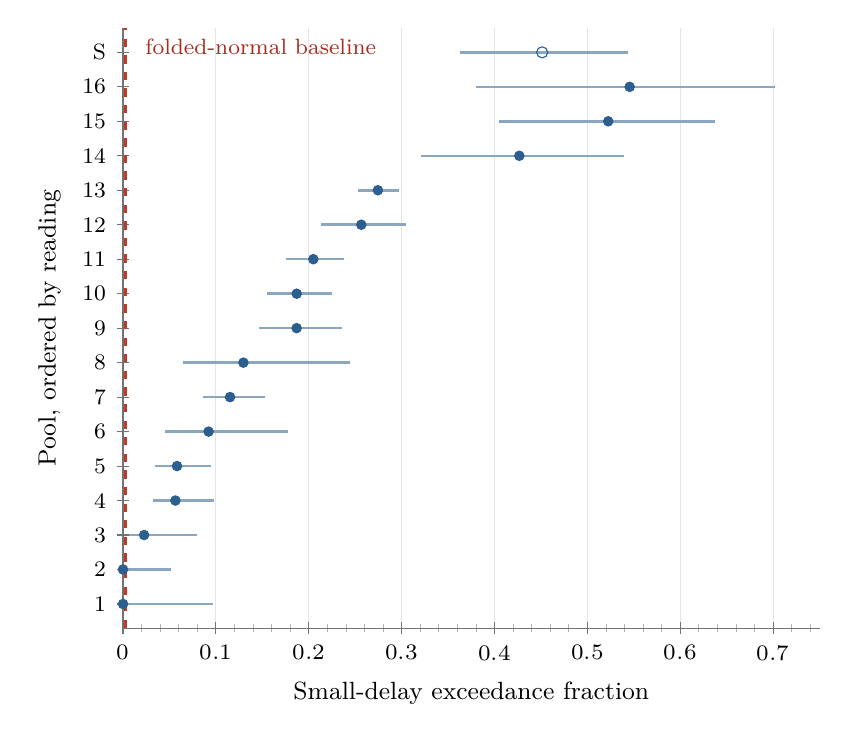
\begin{tikzpicture}
\begin{axis}[
  ltaxis,
  width=0.86\linewidth, height=9.2cm,
  xmin=0, xmax=0.75, ymin=0.3, ymax=17.7,
  xlabel={Small-delay exceedance fraction},
  ylabel={Pool, ordered by reading},
  ytick={1,...,17},
  yticklabels={1,2,3,4,5,6,7,8,9,10,11,12,13,14,15,16,S},
  minor x tick num=4,
  xmajorgrids,
]
% folded-normal baseline
\addplot[ltred, thick, dashed, forget plot]
  coordinates {(0.0027,0.3) (0.0027,17.7)};
\node[font=\footnotesize, anchor=south west, text=ltred!85!black]
  at (axis cs:0.012,16.6) {folded-normal baseline};
% Wilson intervals
\foreach \lo/\hi/\y in {
  0.0000/0.0964/1, 0.0000/0.0513/2, 0.0063/0.0791/3,
  0.0318/0.0982/4, 0.0349/0.0951/5, 0.0453/0.1781/6,
  0.0860/0.1525/7, 0.0642/0.2442/8, 0.1461/0.2358/9,
  0.1545/0.2245/10, 0.1757/0.2375/11, 0.2134/0.3049/12,
  0.2532/0.2966/13, 0.3210/0.5395/14, 0.4049/0.6375/15,
  0.3799/0.7016/16, 0.3627/0.5432/17}
  \addplot[ltblue!55, line width=0.9pt, forget plot]
    coordinates {(\lo,\y) (\hi,\y)};
% point estimates
\addplot[only marks, mark=*, mark size=1.7pt, ltblue, forget plot]
  coordinates {
  (0.0000,1) (0.0000,2) (0.0227,3) (0.0564,4) (0.0581,5)
  (0.0921,6) (0.1152,7) (0.1296,8) (0.1869,9) (0.1870,10)
  (0.2049,11) (0.2565,12) (0.2744,13) (0.4267,14) (0.5224,15)
  (0.5455,16)};
\addplot[only marks, mark=o, mark size=2pt, ltblue, forget plot]
  coordinates {(0.4513,17)};
\end{axis}
\end{tikzpicture}
\caption{Per-pool small-delay exceedance readings with 95\,\%
Wilson intervals, pools ordered by reading; the open marker S
aggregates the seventeen pools below thirty admitted events. The
dashed line is the folded-normal baseline 0.0027.}
\label{fig:perpool}
\end{figure} The
geometry census settles the multiscale proposition's conditionality; 24
of 50 pools host a single trigger scale, 26 host the two or more the
hypothesis of Proposition~\ref{prop:multiscale}(iii) names, and 19 host
three or more. The conservative availability count is therefore the
19 pools, under two fifths, and the proposition is stated as
conditional throughout.\footnote{The two-scale margin is thin. The
census counts scales at two significant figures and the ratio
estimate degrades as adjacent scales approach, so the 26 is the count
most exposed to that rounding and the 19 is the one to rely on.}

\subsection{Tick-stream corroboration and its limit}\label{sec:tickstream}

Direct detection on the per-pool tick stream corroborates the
magnitude; per-block displacements exceed three trailing local
scales in every pool, median pool rate 0.33, so the price law at
block scale is heavy-tailed against trailing-window diffusion
unconditionally, which is directionally consistent with a
price-process component in the firing-based excess rather than an
operator artefact alone. The same exercise fails as a cross-pool
ranking, Spearman $-0.04$ against the firing-based readings,
because the per-block detector is discreteness-dominated in quiet
pools, jump-size medians up to 32 scales beside low rates, the
signature of one-tick quanta over a tiny local scale. The failure
motivates budget row 8 and its admission
constant.\footnote{A crossing-conditioned validator, which would
score the tick stream only where an operator's line was actually
crossed and so inherit the firing-based admission, is the natural
redesign and is not attempted here.}

\subsection{Certifications and cross-checks}\label{sec:certifications}

Five certification probes close the loop between the hypotheses of
Section~\ref{sec:hypotheses} and the census. The era-half
replication splits the era at its midpoint block; the population
reading replicates, exceedance 0.225 against 0.205, while of six
pools with thirty admitted events in each half, three reject the
one-functional null after familywise correction, so (F1) certifies
at population level and binds as a per-pool admission criterion,
with the failing pools carrying per-half statements only. The
refutable implication of (F4) survives its first run; exceedance
shape across cadence strata agrees to a Kolmogorov--Smirnov
statistic of 0.17 ($p = 0.54$, 85 exceedances, matched medians and
ninetieth percentiles), a low-power pass that is now captured and
cheap to rerun. The designated bipower estimator, rerun over the
same events, raises every population cell, 25 to 30\,\% against the
captured realised-variance 18 to 22\,\%, the direction and rough
magnitude row 3's measured inflation predicts, so the captured
columns are confirmed conservative rather than assumed so. Two
cross-checks anchor the inputs. Six census pools are independently
indexed in the operator lake's swap extension; on 555{,}020 shared
era blocks the two tick streams agree within one tick on 91 to
99\,\% of blocks under the verified closing-tick convention, with
one gross outlier flagged as a data-quality defect in one source,
so the tick-stream provenance carries no systematic bias. And the
discreteness admission constant, rebuilt per pool from real
trade-size distributions where swap-level data exists, spans 8 for
fine-trade pools to beyond 32 for coarse ones, bracketing the
synthetic constant 16 of Section~\ref{sec:verification}; the
admission of budget row 8 is per-pool wherever the trade law is
measurable, and coarse-trade pools admit no small-delay reading at
production scales.

\subsection{The second deployment and the cross-venue test}\label{sec:crossvenue}

The instrument was ported unchanged to the population of a second
deployment. An operator-keyed census of Uniswap V3 on Base over the
same era admits 1{,}046 cells across 691 operators on 69 pools, of
which 495 clear the clean-step line-recovery gate at thirty firings
and 227, across 160 operators, clear the stricter bar of the
fingerprinting convention, with recovered trigger fractions again
spanning 0.10 to 0.42. The separating instrument is the clean-step
gate, not the infrastructure filter, which removes almost nothing
at the admission bar; the dense retail and bot population of the
busiest pool passes admission in numbers and largely fails line
recovery,
which is what a census keyed on line-imprinting operators should
show. The read replicates in structure. The clean cells supply
34{,}100 trigger firings, and the small-delay excess sits at 44 to
48 times the folded baseline under trailing local scales, higher
again under the bipower rerun, on an
independent population reading independent contracts, with the
per-pool spread again far beyond binomial noise. It does not
replicate in certification; every pool at the per-pool reading bar
fails the discreteness admission of budget row 8, the scale ratios
running 1.2 to 9.8 against admission constants of 16 to 32 with
each observed reading at or below its pool's own discreteness null,
and the era-half criterion (F1) rejects on the only testable pool,
so this venue-era admits no certified jump reading.

The cross-venue agreement test is read admission-first. One
venue-level pair is testable at the bar, WETH/cbBTC, and it rejects
equality (Fisher $p = 0.0022$); the rejection is fully localised to
the pre-specified admission failure, the Uniswap pool's scale ratio
sitting at 1.2 with a discreteness null near 0.38 against the
observed 0.41, and the within-venue heterogeneity across the
pair's three Aerodrome pools already exceeds the cross-venue gap.
Where admission-comparable readings exist the venues agree. The one
same-pool check powered on both pipelines, the census's own
Uniswap V3 WETH/USDC member read through two independent indexing,
keying, and tick-cache chains, agrees within binomial noise ($p =
0.155$), the port-validity analogue of the provenance cross-check
above; and the one pair powered across the census's PancakeSwap and
Aerodrome members, SOL/cbBTC, agrees across deployments. The certified verdict is that
the agreement claim, that the signal is a property of the pool's
price law rather than of the operators reading it, survives where
the instrument is admitted and is untested, not refuted, where it
is not; a certified cross-venue equality test needs a denser-stream
era or per-swap trade data to sharpen the admission constant.


% =========================================================================
\section{The jump surcharge}\label{sec:surcharge}

The last result joins the three acts. Jumps do more than add a
crossing channel to the intensity layer. A jump fires the trigger
from beyond the line, so every crossing it
causes is settled at a deeper displacement than the same policy
would have paid diffusively, and the placement potentials of
Section~\ref{sec:cost} price the difference exactly.

\begin{proposition}[Jump Surcharge]\label{prop:surcharge}
Under the era model with jumps and the hypotheses of
Section~\ref{sec:hypotheses}, consider an isolated policy, of
$\mathcal{A}_0$ or $\mathcal{A}_2$, with up-trigger displacement
$xh$ whose return convention keeps the upper branch binding at both
the diffusive firing state $xh + O$ and the jump-shifted state $xh +
O + O_J$. The kerf rate gains the additive
term
\[
r_J \;=\; \lambda_J\,
\mathbb{E}\Big[\, \mathcal{C}^{\uparrow}\big(xh
+ O + O_J\big) - \mathcal{C}^{\uparrow}\big(xh
+ O\big) \Big] \;\ge\; 0,
\]
independent of the return point, where $O$ is the monitoring
overshoot of Proposition~\ref{prop:monitoring}, $O_J$ the straddle
depth of Section~\ref{sec:jumpbranch}, $\lambda_J$ the
occupation-averaged jump-crossing intensity of
Lemma~\ref{lem:straddle}, and the expectation is taken under the
jump-crossing law at that same weighting. In the narrow limit, on the event that the
fired state remains inside the range,
\[
r_J \;=\; \lambda_J\, \mathbb{E}\Big[\ln
\frac{(1-x)\,h - O}
{(1-x)\,h - O - O_J}\Big]
\;\ge\; \frac{\lambda_J\, \mathbb{E}[O_J]}{h},
\]
with the down branch symmetric. Straddles that carry the state
beyond the range boundary pay the corner value of the exact
potentials in the isolated class, and the swap-mediated cost at the
landed share gap otherwise.
\end{proposition}

\begin{proof}[Proof sketch]
The per-event cost difference between the jump-shifted and the
diffusive firing state telescopes through the placement potentials
of Section~\ref{sec:cost}, cancelling the return point; positivity
is strict monotonicity of $\mathcal{C}^{\uparrow}$, and the
narrow-limit form is the logarithmic potential. Full proof in
Appendix~\ref{app:floors}.
\end{proof}

\emph{In words, every jump crossing of an isolated policy whose
binding branch does not switch pays at least its straddle depth over
the half-width, in log-value, on top of everything the diffusive
floor already charges, and no return convention avoids it.}

The beyond-range clause carries a scope note. A landing beyond the
range boundary leaves single-sided holdings from which no
price-containing equal-width range can be minted, so its
isolated-class log-cost is infinite; any jump law with support
beyond $(1-x)\,h$ therefore gives every band-maintaining
isolated-class policy an infinite kerf rate, the
value-flux ledger staying finite, and isolated-class rates under
such laws are quoted only under a stated per-event cap
(Section~\ref{sec:verification}).

Two consequences follow. The emission-based isolated floors of
Sections~\ref{sec:fixed} and~\ref{sec:width} harden by the additive
term $r_J$, since the surcharge is pathwise and per-event. The
swap-mediated floor of Section~\ref{sec:swap} hardens too, but not
by $r_J$; a deeper landing enlarges the share displacement its
impulse must correct, and that cost is the execution one of
\eqref{eq:swapcost}. The
retention collapse of Section~\ref{sec:collapse} is unaffected,
because retention deletes the surrender, straddle-deep or not. The
surcharge is also measurable. Its two inputs, the jump-crossing rate
and the straddle law, are the functionals the instrument of
the third act identifies per pool
(Theorem~\ref{thm:smalldelay} and Corollary~\ref{cor:tailshape}),
with the check-weighting caveat of Section~\ref{sec:response}
applying to the rate; the per-pool magnitudes belong to the
population read (Section~\ref{sec:evidence}) and its disclosure
gate.

The ledger can be worked on a live book. Take the operator's
WETH/TOSHI position from the production anchor of
Section~\ref{sec:verification}, a 24 basis point pool at tick
spacing 200 with median position value near \$535;
Table~\ref{tab:worked} runs the ledger at the anchor window's
measured parameters. The concavity leg, the price of holding
concentrated inventory at that width and volatility, is recoverable
only through fees and emissions; the event floor at the pool's own
fee sits below it by the measured factor $0.24$, which is
$\eta/(2\rho)$ at this geometry, the ordering of
Proposition~\ref{prop:legs} at production numbers; and the realised
event-leg rate runs at twice its class floor, with
the measured geometry, late trigger and small correction, in the
corner Proposition~\ref{prop:return} prices as cost-optimal in
direction. The remaining gap is a control lever. In a subsequent
trigger experiment on the same pool the operator moved the trigger
fraction from one quarter of width to $0.12$, the $x$ of
\eqref{eq:rswap} from $0.5$ to $0.76$, and the churn share of gross
revenue fell from $23.6$ to $14.7$ per cent with net revenue per
day unchanged, the direction \eqref{eq:rswap} predicts.

\begin{table}[H]
\centering
\caption{The ledger worked on the WETH/TOSHI book.}
\label{tab:worked}
\begin{tabular}{@{}llr@{}}
\toprule
Quantity & Form & Measured \\
\midrule
narrow-range parameter & $\rho$ & $0.0051$ \\
sqrt-price volatility & $\sigma_s/\bar s$ & $0.25$ per $\sqrt{\text{yr}}$ \\
concavity leg & $\sigma_s^2/(2\bar s h)$ & $613\,\%/\text{yr}$ \\
event floor, pool fee & $\eta\,(1-\rho_w)^2\sigma_s^2/w^2$ & $144\,\%/\text{yr}$ \\
leg ratio & $\eta/(2\rho)$ & $0.24$ \\
realised event-leg rate & \eqref{eq:kdef} summed per year & $290\,\%/\text{yr}$ \\
trigger fraction, correction & medians & $0.69$, $0.05$ \\
\bottomrule
\end{tabular}
\end{table}

% =========================================================================
\section{Numerical verification}\label{sec:verification}

Each act ships its own dependency-free reference implementation
at a fixed seed, with captured output as the regression target, a
fourth surface evaluates the first two acts on the operator's
production history, a fifth replays the exact layer against
unmodified production bytecode on three deployments and two chains, a
sixth replays
the discrete-bin algebra of Appendix~\ref{app:lb} against that
venue class's unmodified home deployment, a seventh calibrates
the instrument and stress-tests the floors on synthetic ground
truth at simulation scale, and an eighth carries the exact layer and
the third-party identity onto Ethereum mainnet at a twelve-second
block; nothing below
consumes on-chain data except the anchor, the fork suites, and the
third act's probes, which read the population layer of
Section~\ref{sec:evidence}.

The eight surfaces are complementary rather than independent
replications, and the distinction matters for how much each adds.
The harnesses check implementations against formulas derived in this
paper, so they test agreement and not the derivations; the anchor's
operator is the present author, which is why the same identity is
evaluated on third parties below; and the seventh surface's
synthetic populations carry operator geometries drawn from the
second deployment's census, so its calibration inherits that
population's geometry rather than testing it. None of the eight
replaces a proof, and none establishes validity outside the stated
hypotheses.

The first act's harness begins with the amplitude. The two-branch
amplitude \eqref{eq:branches} is checked against the mint-minimum
arithmetic over 20{,}000 random parameter draws with both branches
evaluated, agreeing to $2.1 \times 10^{-12}$ relative, the corner
values of Corollary~\ref{cor:corners} to $1.1 \times 10^{-14}$, and
the monotonicity threshold of Proposition~\ref{prop:mono} by
bisection to $6.4 \times 10^{-5}$. The pathwise identity
\eqref{eq:dissipation} is reproduced on a simulated path with 250
impulses at a relative residual of $1.551 \times 10^{-14}$, the
identity being exact path by path, which is also what
Proposition~\ref{prop:discretefloor} exploits. The
remaining checks exercise the occupation-offset bound of
Corollary~\ref{cor:occupation} on a simulated tick path together
with the monitoring dichotomy of
Proposition~\ref{prop:monitoring}(i), near-continuous monitoring
concentrating the firing offset and coarse monitoring restoring
uniformity, and the scale-function direction split, reproduced within
Monte Carlo and discrete-step overshoot error.

The second act ships two artefacts, both standard-library Python
at fixed seeds. The scoping probe
simulates the centred fixed-width family at four triggers
and matches the exact coefficient \eqref{eq:cx} within 3\%,
minimum measured $c = 2.38$ at $x = 0.72$ and $\rho =
0.05$; its extension simulates off-centre re-placements against the
two-argument amplitude, ratios $0.99$ and $1.08$, and grid-searches
the full three-parameter renewal family analytically, minimum
$c = 2.397$ at the symmetric point $(-0.72, 0.00, 0.72)$, a family
whose single shared target cannot express the per-side reflection
targets of Proposition~\ref{prop:sharp}.

The reference harness checks the algebraic layer first. The placement-family
potential identity holds across twenty thousand random equal-width
geometries with worst error $2.7\times10^{-12}$, the
share-potential identity across twenty thousand random width pairs
with worst error $8.9\times10^{-16}$, machine precision, confirming
Theorem~\ref{thm:share} is an identity rather than an
approximation, and the free locus across two thousand solved
ratio-preserving widenings with worst cost $2.7\times10^{-14}$. The
floor layer follows. The corridor constants quoted after
Theorem~\ref{thm:fixed} and its analytic corollary are reproduced,
the centred Monte Carlo sweep and the renewal grid put every member
above $c_{\min}$, and the widen-slide adversaries against the
width-uniform floor at cap ratio two reach $5.51$ at best against a
floor of $5.12$, the remaining margin consistent with a floor
approached from inside the class, with a longer run of the
full-recentre configuration at $644$ paid events measuring $7.02
\pm 0.28$. The clock and drift bounds of Lemma~\ref{lem:clock} hold
over five thousand random geometries. In the swap class the
constant $A$ matches Table~\ref{tab:production}, edge-hugging
converges to the fee-only floor at ratio $1.005$, and Monte Carlo
return-point policies match \eqref{eq:rswap} to 2\% at the deployed
convention and to 14\% at the near edge, where discrete-step
overshoot lengthens cycles, the near-edge policy sitting 2\% above
the floor, consistent with the tightness of
Proposition~\ref{prop:return}.
No tested policy in any family beats its class floor.

The third act's synthetic harness seeds each check
independently, so extensions never disturb
captured draws. The delay-law mixture of
Proposition~\ref{prop:reproduction} is reproduced to a relative error
of $6 \times 10^{-15}$, and the joint flat-entry law is confirmed by
exact L\'evy first-passage sampling with no path discretisation,
Kolmogorov--Smirnov statistics at the sampling floor for
$n = 49{,}415$. The full pipeline, threshold operator, trailing
bipower scale with candidate exclusion, exceedance and jump-share
estimators, recovers a planted jump share inside
Theorem~\ref{thm:smalldelay}'s bracket and a planted Pareto tail
index within a Hill error of 0.21 on 224 exceedances. The
delay-invariance dichotomy separates a penetration operator (ratio
0.033) from a lag operator (2.3, the meander factor included), and
jump enrichment measures 0.85 against 0.54. The agreement test
holds empirical size 0.043 to 0.045 at nominal 0.05, the
discreteness sweep delivers $c_{\mathrm{tick}} = 16$ under a
trade-quantum null, and Cox checking shifts the small-delay jump
share while moving the recovered tail index by 0.07, inside noise,
the level-shape split of (F4) verified end to end.

A fourth surface anchors the first two acts in production data;
the operator is the present author. The position-manager history,
135{,}538 recorded rebalances with per-event burn, swap, mint, and
residual amounts over the first 53 days of its era, is evaluated
against the theory with no synthetic input. On the 78{,}908
events whose value chain closes without drawing on the standing
residual balance, the share-potential identity holds with median
absolute error $5.7 \times 10^{-17}$ in $k$, machine precision on
production events, and residual conservation holds on all of them;
the two fifths of events that do draw on the balance are the
retention architecture of Section~\ref{sec:collapse} operating
live, priced in the rate evaluation but excluded from the identity
subsample, whose hypothesis is isolated holdings. Per pool, no
volatile-pair book runs below its class floor at a uniform
production fee anchor, distances to floor are set by correction
size and width as the benchmark reading of Section~\ref{sec:swap}
predicts, and measured median trigger fractions, 0.22 to
1.14 across pools, confirm the late-firing direction.
Figure~\ref{fig:anchor} plots realised rates against class floors.
The captured
output supplies the worked example of Section~\ref{sec:surcharge}.

The identity is therefore also evaluated on third-party
operators: every same-transaction
re-placement on the census pools of both deployments over the
census era, reconstructed from public burn and mint events with
the transaction sender attached, author and infrastructure
addresses excluded. On the isolated interior re-placements that
survive the anchor's own event discipline, 253 on Aerodrome
Slipstream across ten operators and 345 on Uniswap V3 across
eight, the identity holds with median absolute error $1.1 \times
10^{-16}$ in $k$ on each venue, the same machine precision as the
anchor, with the recovered price self-consistent to $2.5 \times
10^{-14}$ on Uniswap V3 and $1.6 \times 10^{-11}$ on Slipstream;
the error tail (99th percentile near $4 \times
10^{-4}$) is in-transaction fee collection contaminating the
isolated-holdings hypothesis at the margin.
Twenty-two further isolated re-placements on Ethereum mainnet,
read the same way over the mainnet era, hold at median $7.9 \times
10^{-17}$ with maximum $2.0 \times 10^{-14}$, so the identity is
evidenced on three venues across two chains. A further 2{,}385 and
33{,}008 single-sided limit placements satisfy the identity
trivially, and the excluded classes, fee-compounding top-ups
first among them, are tabulated in the captured output. The
identity subsample is small because the behaviour is rare among
third parties, not because it fails; no surviving event on either
venue misses the prediction.

\begin{figure}[H]
\centering
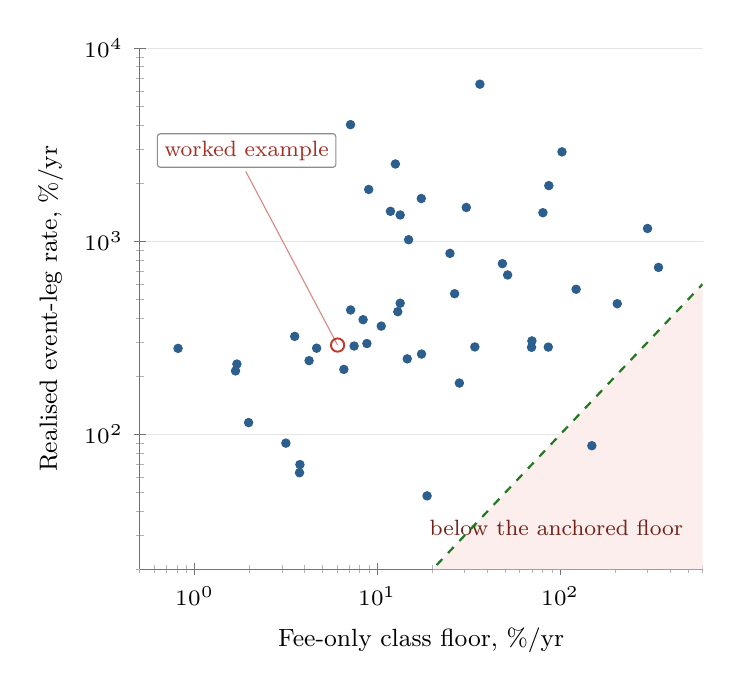
\begin{tikzpicture}
\begin{loglogaxis}[
  ltaxis,
  width=0.72\linewidth, height=8.2cm,
  xmin=0.5, xmax=600, ymin=20, ymax=10000,
  xlabel={Fee-only class floor, \%/yr},
  ylabel={Realised event-leg rate, \%/yr},
  ymajorgrids,
]
% below the identity, where the uniform anchor overstates the floor
\path[fill=ltalerttint] (axis cs:20,20) -- (axis cs:600,600)
  -- (axis cs:600,20) -- cycle;
\node[font=\footnotesize, anchor=south east, text=ltred!60!black]
  at (axis cs:540,26) {below the anchored floor};
% the floor itself
\addplot[ltgreen!75!black, line width=0.8pt, dashed, domain=0.5:600,
  forget plot] {x};
\addplot[only marks, mark=*, mark size=1.5pt, ltblue, forget plot]
  coordinates {
(7.12,440.46) (85.82,282.93) (204.63,474.62) (24.88,865.03)
(102.02,2902.43) (121.9,563.94) (7.11,4014.96) (28.01,184.27)
(34.04,283.44) (6.54,216.82) (36.28,6507.01) (17.39,260.37)
(3.76,69.7) (26.39,534.63) (18.65,47.99) (148.61,87.28)
(299.65,1163.86) (8.94,1853.76) (69.52,282.2) (13.29,477.5)
(69.85,304.52) (12.89,431.47) (14.78,1017.96) (4.64,279.3)
(8.74,295.12) (3.52,321.49) (17.34,1664.23) (11.76,1428.58)
(10.47,363.37) (4.22,240.73) (51.43,668.64) (343.93,731.88)
(3.15,90.01) (8.33,392.31) (48.16,765.34) (14.53,245.87)
(80.22,1405.11) (12.51,2511.81) (86.43,1941.44) (3.74,63.24)
(13.29,1367.3) (7.44,286.6) (30.56,1495.66) (1.67,212.96)
(1.7,231.12) (1.97,114.97) (0.81,278.59)};
\addplot[only marks, mark=o, mark size=2.4pt, ltred, line width=0.7pt,
  forget plot] coordinates {(6.04,289.89)};
\draw[ltred!60, line width=0.4pt] (axis cs:6.04,289.89) -- (axis cs:1.9,2300);
\node[ltcallout, anchor=south west, text=ltred!85!black]
  at (axis cs:0.62,2400) {worked example};
\end{loglogaxis}
\end{tikzpicture}
\caption{The production anchor's per-pool realised event-leg rates
against the fee-only class floor at the uniform $\eta = 10^{-4}$
anchor, the dashed identity, with the worked example's book marked
open. Points inside the tinted region are pegged pairs, where the
uniform fee anchor and the realised-variance $\sigma$ overstate the
floor rather than the book undercutting it.}
\label{fig:anchor}
\end{figure}

A fifth surface replays the exact layer against production
bytecode. The fork suite of Section~\ref{sec:forksuites} replays four
results against two unmodified position managers on Base and, in the
mainnet arm, against the Uniswap V3 manager on Ethereum at a
twelve-second block.
On pseudo-random width pairs the re-mint liquidity equals the
binding-side minimum and the mint amounts match the V3-exact
prediction to a few wei on both deployments. The two-branch
amplitude is realised as whole-tick translates of the old range
with the pool price placed at the translate's midpoint, so the only
model gap is the translate's width factor, and the closed form
\eqref{eq:branches} agrees within that budget, twelve to
forty-four parts per million at tick spacing ten and one to four and
a half parts per thousand at spacing one hundred, with the binding side
per branch as Lemma~\ref{lem:binding} states. The corner values
are quantisation-free, the corner ratios of
Corollary~\ref{cor:corners} agreeing to the wei with the recentred
corner mint reverting empty on both managers, and the identical
re-placement of the free locus costs one raw token unit.

A sixth surface replays the discrete-bin algebra against its own
deployment. The second fork suite replays Appendix~\ref{app:lb}
against an unmodified Liquidity Book pair on the class's home chain.
The bin price law is bit-exact against
the pinned source libraries at ids spanning the active bin by five
thousand, with the offset anchor exact and the step ratio inside
the power library's own truncation bound; the constant-sum depth,
the atom amplitude, and the live fee quote and single-price
execution are exact to the wei; and the per-traversal loss matches
its price-ratio form with zero relative gap at the programme's
fixed-point tolerance.

The discrete-bin algebra is also evaluated on third-party
operators. Over the three million blocks ending at the fork
pin, every withdrawal and redeposit pair on the class's home chain
falling within fifty blocks was reconstructed from public events,
admitted only when the two transactions share a sender, neither
contains a swap on the pair, and a closed-interval log query over
the pair returns exactly those two transactions, so that no third
party mutated the touched bins between them. 77 sequences survive,
on nine pairs across twenty-one distinct senders. The burn law is
exact in all 1{,}406 bin legs, the mint law holds with median
residual $7.0 \times 10^{-22}$ and maximum $1.0 \times 10^{-20}$,
and the composition fee, its protocol split, and the final-shares
rule are exact on all forty-eight events that carry one. One
caution follows from the exercise. The home deployment predates the
source repository's correction to the composition-fee divisor, so
the deployed final-shares rule divides by the original bin
liquidity where the read commit divides by that liquidity plus the
net fee; asserting the commit form against this deployment measures
the version difference, at most $5.5 \times 10^{-3}$ here, rather
than the rule. The deployed form is the object, and the difference
is reported beside it in the captured output.

A seventh surface calibrates the statistical layer on synthetic
ground truth. Where the first six surfaces assert identities, this
one measures the instrument; the worlds are diffusion with planted
jump measures, no price model entering as an assumption, the
populations carry operator geometries drawn from the second
deployment's census, and the actual inversion pipeline of
Appendix~\ref{app:estimators} runs unchanged on the synthetic
firing records, each simulator validated event-exactly against the
shipped harnesses before use. The recovered jump share sits inside
the bracket of Theorem~\ref{thm:smalldelay} in every cell of every
sweep, 120 pool-inversions per planted world across population,
era-length, and delay-cut sweeps. The bias is the resolution floor
and behaves as the theorem prices it, flat in population and era
and moving only with the delay cut, negative by the straddle mass
below resolution and correctable through the recovered tail;
precision is admitted-event-limited rather than operator-limited,
a read to within two hundredths needing roughly two thousand
admitted small-delay events per pool-era, which at production
firing rates means on the order of tens to a hundred operators or
pooled-era accumulation;
and the tail read carries the finite-reference upward bias of its
Hill kernel, with a stated breakdown regime, sparse heavy tails
becoming unreadable below roughly four hundred thousand blocks of
era at the thinner planted rate.

The same surface maps the statistical results beyond the shipped
harnesses and ran the policy search behind
Proposition~\ref{prop:sharp}. Across 141 planted jump, delay, and
drift configurations, the flat-kernel form of the small-delay
bracket holds on 4{,}669 of 5{,}046 admissible readings, every
failure marginal and confined to high cut multipliers against
small jump scales, exactly the regime in which
Corollary~\ref{cor:tailshape} prescribes the estimated-kernel form
in place of the flat leading order; the consistency clause of
Theorem~\ref{thm:smalldelay} manifests as convergence in the
resolution ratio, block-quantised delays bounding the joint limit
away; and the surcharge premium of
Proposition~\ref{prop:surcharge} matches its potential form per
event to a few parts per thousand with the lower bound holding
throughout, beyond-range landings carried under a stated per-event
cap of ten log-units. On the floor side, four independent instruments
agree, the exact cycle algebra of the reflection family, a
grid policy iteration with no structural restriction, a
four-parameter renewal sweep, and a Monte Carlo zoo of 139
policies with exact mint arithmetic; the tested reflection and
near-chattering members approach the floor across the simulated
regimes, no member undercuts the
era-banded floor for its visited band, and in planted jump regimes
the infimum rises with tail weight while the optimal reflection
point moves inward from the tangency, guarding against straddles.

An eighth surface carries the exact layer and the third-party
identity onto Ethereum mainnet, at a twelve-second block and under a
different sequencing regime. The fork track and the identity events
are reported above. What the arm adds beyond them is a two-sided
floor scatter. On the fifth to the third of mainnet firings that
carry their corrective swap in the same pool, the swap's own
constant-liquidity arithmetic marks the position before the swap, so
the realised event cost is measured rather than bounded as it is on
Base. Seven cells clear the firing bar, three operators over spans of
eighteen to a hundred and fifteen days and 566 swap-carrying firings;
all seven sit above the uniform fee-only floor at the anchor's fee,
at a median score of $57.6$, and six of the seven sit above their own
pool's fee tier. The sample is small and is not a census.

The same arm measures whether the event leg is somebody else's
revenue. Against a within-block null, rebalance firings are neither
backrun nor sandwiched on either chain, every adjacency ratio sitting
at or below one, $0.97$ and $0.81$ on Base against $0.52$ and $0.77$
on mainnet; the raw shares alone would have read the other way, which
is why the null is the statistic and the share is not. Mainnet
firings sit late in their block, a frontrun ratio of $1.41$ against a
backrun ratio of $0.52$, which reads as low-priority ordering rather
than extraction and places the mint near the block's closing price,
the convention the tick cache already assumes. The dissipation priced
here is therefore not, on this evidence, an artefact of anyone taking
the other side of it.


% =========================================================================
\section{Machine verification}\label{sec:machine}

The verification package holds three kinds of artefact, and they are
not interchangeable evidence. Two are executable against deployed
bytecode, one is a kernel-checked proof, and the fixed-seed harnesses
of Section~\ref{sec:verification} are finite-precision
implementations checked against the stated formulas. The fork suites
of the fifth and sixth
surfaces run the exact layer against production bytecode, so the
arithmetic they check against is the venue's rather than a model of
it; this section says how they are built and what a reader has to do
to rerun them. The formalisation is not a verification surface at all.
It machine-checks the theorem layer over the reals, so a kernel
checks those proofs, and it is reported here because the two
artefacts answer complementary questions.
Fixed-point pool arithmetic is outside the formalisation by
construction, and the paper's stochastic steps are outside the fork
suites by construction.

\subsection{The fork suites}\label{sec:forksuites}

Twenty tests across four contracts, all against unmodified
deployments at pinned blocks. Two tracks on Base at block
$45{,}000{,}000$ replay the exact layer against the Aerodrome
Slipstream and Uniswap V3 position managers on the same
tick-spacing-one-hundred WETH/USDC book, four tests each. A third
track on Ethereum mainnet at block $25{,}200{,}000$ replays the same
four results against the Uniswap V3 manager on the
tick-spacing-ten WETH/USDT book, where the corner ratio agrees to the
wei and the free locus costs zero raw units against Base's one. One
track on
Avalanche C-Chain at block $92{,}430{,}000$ replays
Appendix~\ref{app:lb} against the bin-step-ten WAVAX/USDC pair of the
discrete-bin class's home deployment, eight tests. The mainnet pair is
forced rather than chosen, the suite's tolerances being absolute raw
units calibrated for a six-decimal token1, which mainnet USDC/WETH
inverts. The Base pin sits
inside both the census era and the production anchor's amounts window,
so the fork tier, the census, and the anchor share an era.

Predictions come from an exact-tick-math reference contract synced to
the live pool's state at the pinned block, never from a linearisation,
so a disagreement is a disagreement with the deployed arithmetic and
not with an approximation of it. Where quantisation makes exactness
unavailable the tolerance is stated with its budget and the residual
is logged, which is why the two-branch
amplitude is reported at parts per million and per thousand by tick
spacing while the corner ratios and the mint minimum are asserted to
the wei. A clean checkout reproduces every fork result in the previous
section; the captured run, with the test-to-result map, is the suite's
regression target, and any archive-capable endpoint for each chain
suffices, since the pins fix the state.

\subsection{The formalisation}\label{sec:lean}

The theorem layer is machine-checked in Lean 4 against mathlib, over
the reals. Every theorem stated inside the development is checked by
the Lean kernel, subject to the foundational axioms the accompanying
audit records, which closes on the three standard ones. The scope is the idealised model, and the
mapping from file names to the paper's numbering ships with the
development.

What is proved is the algebraic and variational spine. The central
law is formalised in full, at any width pair and any admissible
target range, together with the non-negativity of the kerf and the
free locus as an exact characterisation;
the abstract half, that for two share pairs summing to one the smaller
cross ratio is at most one with equality exactly when the pairs agree,
is isolated first and is the entire source of both. The amplitude
layer follows, its two branches proved as the exact difference between
withdrawn and re-minted value, not posited, with the corner
values, the exact fractional slopes, and the down-branch monotonicity
threshold in its iff form. The placement-family potentials carry their
monotonicity and the impossibility of a free round trip. In the second
act the corridor is checked, with the tangency constant coming out
exactly two as an infimum and with its analytic corollary, and the
impulse inequality is checked in the share coordinate as well, where
it is exact at every width and carries no narrow-limit correction;
that second coordinate is what shows the constant is not an artefact
of the first. Both policy families are checked against the floor, as
are the swap sandwich with its constant and its class-coverage
argument, the retention collapse, the leg comparison, and the jump
surcharge. In the third act the monitoring layer's two exact
integrals are proved, and so is the analytic core of the
exact-reproduction identity discussed in
Section~\ref{sec:diffusive}.

What the formalisation does not carry is the assembly. The floors of
Sections~\ref{sec:fixed}--\ref{sec:swap} are stated under continuous
monitoring, and the step from the corridor and the impulse inequality
to a rate bound runs It\^o between impulses, telescopes, and closes
with a martingale argument, none of which mathlib supports. The
corridor, the impulse inequalities, and the tangency constant are
machine-checked; the floors those ingredients assemble into are not.

What is machine-checked in full is the counterpart,
Proposition~\ref{prop:discretefloor}. For a quadratic verification
function the second-order expansion is an exact identity with no
remainder, so under discrete monitoring the scheme runs pathwise on
finite sums, and the bound follows at each of the three classes with
no stochastic analysis at all. That proposition entered the paper
because the formalisation established it, and it is the one floor
statement here whose proof a kernel has checked end to end.

The remaining gaps are stochastic, and the development records
them. Theorem~\ref{thm:dissipation} needs the
local-time field of a continuous semimartingale and It\^o--Tanaka for
a difference of convex functions, neither of which mathlib carries.
Proposition~\ref{prop:intensity} needs first-passage theory for the
same reason, as does the renewal-reward step behind the cycle
constants, so the family-optimum constants of
Section~\ref{sec:fixed} are the harness's rather than the
formalisation's. The instrument's Gaussian branch estimates are not
formalised, only the deterministic assembly of their conclusions.
Offset uniformity and exact reproduction are each proved up to one
standard step that is carried as a hypothesis, the identification of a
pushforward density with a lattice sum in the first case and an
improper change of variables in the second. Nothing downstream of
Theorem~\ref{thm:dissipation}'s impulse term depends on the
unformalised parts.

Table~\ref{tab:evidence} sets the two sections' surfaces beside each
other by the layer of claim each one reaches, with what it does not
reach recorded in the same row. The rows are independent, and the
paper's strongest statements are the ones several of them support at
once.

\begin{table}[H]
\centering
\caption{The evidence ledger by claim layer.}
\label{tab:evidence}
\begin{tabular}{@{}lp{0.24\linewidth}p{0.24\linewidth}p{0.24\linewidth}@{}}
\toprule
Layer & Evidence & Establishes & Does not establish \\
\midrule
algebraic & the formalisation and the seeded harnesses & the identities and the impulse inequalities & the stochastic assembly above them \\
contract & the fork suites, four deployments on three chains & agreement with deployed arithmetic & anything about populations \\
synthetic & fixed-seed simulation and the calibration surface & estimator behaviour against planted truth & that a real price law is the planted one \\
production & the operator's own event history & agreement on the recorded events & a law for venues not read \\
population & the admitted census cells & conditional per-pool readings & recovery of the full jump measure \\
\bottomrule
\end{tabular}
\end{table}

% =========================================================================
\section{Discussion}\label{sec:discussion}

\subsection{The ledger and the benchmark frame}\label{sec:legs}

The dissipation ledger sets two cost layers side by side in one
forward expansion. The concavity leg is the slot the
loss-versus-rebalancing literature occupies,\cite{milionis2022}
benchmark-relative and generated by holding a concave payoff against
a continuously rebalanced reference; the event leg is generated at
re-placement instead, and is attributed to the venue's arithmetic and
the operator's own parameters. Questions of venue design
and of operating policy are questions about the event leg, the term
the policy's own parameters enter. The event leg is also an
instrument; its firing statistics invert for the price law and for
the policy, as OF demonstrates and as
Sections~\ref{sec:ident}--\ref{sec:evidence} carry out; the
source-attributed firing record supplies the observables that
inversion needs, which a benchmark-relative cost alone does not. Fees and
emissions enter the completed ledger as revenue; the concavity leg,
the event leg, and the actuation layer of
Proposition~\ref{prop:monitoring} leave as cost. Each term is
measurable from public data.

\subsection{Limitations}\label{sec:limits}

The specialisations are stated for V3-style geometry and make no
universality claim beyond it. Within the class the exact layer is
asserted against three production deployments on two chains
(Section~\ref{sec:verification}), and the venue presentation is
instantiated on one discrete-bin class whose algebra is in turn
asserted against that class's unmodified home deployment
(Appendix~\ref{app:lb}), with no population read there; other
architectures enter through Section~\ref{sec:recipe} and must be
reconstructed from their own source.

The identity is stated for continuous semimartingales, with jumps
handled by the extension of Section~\ref{sec:jumps}; the
jump-crossing term is calibrated per pool by the third act's
instrument, behind its disclosure gate.

The offset lemma is conditional on regularity of the firing-state
density, and the degenerate continuous-monitoring case shows the
condition cannot be dropped. The independence of the corrective
displacement from the coarse state holds to the fee-order error
carried from OQM.

The second deployment's census era carries no certified jump reading.
Every pool at the per-pool bar fails the discreteness admission,
scale ratios of 1.2 to 9.8 against admission constants of 16 to 32,
and the era-half criterion rejects on the only testable pool. The
cross-venue comparison of Section~\ref{sec:crossvenue} is therefore
read admission-first, and its equality claim survives where the
instrument is admitted and is untested rather than refuted where it
is not. A venue-scale replication of the population read is
outstanding, and the single certified census is the binding
constraint on the third act's generality.

The mainnet arm reads a venue where the behaviour itself is rare.
Active liquidity management there fires about thirty times less often
than on Base, roughly $11{,}700$ firings over the era against
$364{,}098$, so twenty-nine cells clear the firing bar and no mainnet
census is available; the third act's population tiers are blocked by
that sparsity rather than by the method, which is now measured rather
than assumed. Two mainnet-specific filters are measured and not
applied here. Just-in-time positions are $12.9$ per cent of mainnet
position events against $0.2$ per cent of Base's, so a mainnet census
must classify and exclude them; and only $32$ per cent of mainnet
firings carry their corrective swap in the pool, the rest routing
through aggregators, which leaves their value chain unclosable from
the pool's own logs and splits the population into an identified part
and an unidentified one. Of the fifty-five busiest pools at the
reading bar, eight carry V3 event signatures without belonging to the
V3 factory and are excluded rather than mixed in.

The delay cut is matched in wall-clock seconds and not in blocks,
because Theorem~\ref{thm:smalldelay} bounds how far a price moves
while the operator is uncorrected, which is elapsed time against
diffusion rather than the chain's accounting unit. Base's ten-block
cut is twenty seconds, so the mainnet cut is $1.67$ blocks, and a
small-delay class under two blocks wide is not powered on this
population; the cross-chain delay-cut equivalence test is therefore
not attempted. The mainnet discreteness admission is not computed
either, so no mainnet reading is quoted against the admission
constants of Section~\ref{sec:crossvenue}.

Population-level claims are inherited with their published scope.
Trigger geometry transfers across operators, while the first-passage
slope law is pinned on a single control operator, and nothing here
upgrades that.

Further limits bound the third act. Identification beyond integrated tail
functionals is conditional on per-pool geometry counts that
production supplies in a minority of pools at the conservative
census count; the multiscale reconstruction is
therefore a conditional result plus a measured census, not a
blanket capability, and I claim no recovery of the full jump
measure. The level of the jump rate is check-weighted under Cox
monitoring; shapes are clean under the exclusion restriction, whose
refutable implication survives its first run at limited power
(Section~\ref{sec:certifications}). Per-pool readings
below the discreteness admission are quantisation measurements, the
quantisation channel of OQM, not jump measurements, and are
excluded rather than reinterpreted; the admission now has a
venue-scale demonstration, the second deployment's era placing
every pool at its reading bar within one decade of the tick
quantum, so budget row 8 excludes an entire venue-era at once
(Section~\ref{sec:crossvenue}). Era discipline binds
throughout; the population's own policy drift means per-era
statements only, and the era-half replication certifies (F1) at
population level while failing it in half the testable pools, so
finer-than-era homogeneity is a per-pool admission criterion, not
an assumption (Section~\ref{sec:certifications}).

Dollar significance is deliberately out of scope. The identity
prices structure, not size; the event leg's share of aggregate
venue flow is a census quantity for the population line, and no
result here depends on its magnitude.

\subsection{Operating and design implications}\label{sec:implications}

For an operator the results reduce to three rules, all of them
directional and all of them under the execution model. The trigger
should be late, the direction the dwell rules of production
populations already run in, though nothing here makes a deployed
dwell rule optimal once revenue, out-of-range exposure and churn are
counted. The correction should be small
and the width large within mandate, and the benchmark score of
Section~\ref{sec:swap} prices those two choices against the
floor. Nothing in the isolated-class analysis, including $x^* =
0.7153$, applies once swaps are on.

For a designer the results place the decisive choice in the
architecture. The floor's existence is a consequence of emission, and the
retention architecture removes it from the system-value ledger
altogether, at the residual costs Section~\ref{sec:collapse}
itemises; below that choice, the
quantisation menu prices the placement and sizing rules per event
and the cadence term prices the monitoring layer. The design
question is whether the architecture keeps the floor, not how
closely an operator can approach it.

\subsection{Consumers}\label{sec:consumers}

Within the paper the loop closes at Section~\ref{sec:surcharge},
the jump surcharge priced by the instrument's own functionals.
Beyond it, the fingerprinting instrument gains a
price-law-conditioned null, an operator's overshoot tail against
its pool's measured integrated jump-tail functional, and the
defence stated alongside that instrument in OF applies
unchanged, a sharper null tightening what jitter has to
conceal rather than removing the cover it gives; risk mandates
gain a per-pool
jump-tail estimate as a direct input to width and trigger
choices; the volatility-oracle channel is absorbed as
Proposition~\ref{prop:diffusive}; and the emission-side
economics of the ledger upgrades its decision metric from
emissions over the concavity leg alone to emissions over the sum
of the concavity leg and the floor, the elasticity of the ratio
unchanged.\cite{ryan2026lvr}

\subsection{Future work}\label{sec:future}

On the measurement side, the placement-wedge attenuation and
cadence-degradation predictions of Section~\ref{sec:lemma} are
testable on existing data. On the instrument side, the
open items are the redesigned crossing-conditioned tick-stream
validator that the discreteness diagnosis demands, the drift
diagnosis for the pools the era-half replication flags, the
multiscale reconstruction beyond integrated tail functionals where
the geometry census permits it, and a certified cross-venue
equality test, which the executed port of
Section~\ref{sec:crossvenue} shows to need a denser-stream era or
per-swap trade data on the second deployment. That deployment's
census itself sits outside this paper's disclosure gate; over the
same era, an operator-keyed census of Uniswap V3 on Base admits
1{,}046 pool-operator cells across 691 operators on 69 pools, 227
clean line-recovery cells across 160 operators at the
fingerprinting paper's bar, an independent evidence surface built
by this paper's own pipeline. On the portability side, each new
venue enters the same formula through its own discontinuity set,
and the recipe of Section~\ref{sec:recipe} is the working form
of that programme.

% =========================================================================
\section{Conclusion}\label{sec:conclusion}

The paper proved one law and developed it in three directions. The
share-potential identity prices composition motion exactly; the floor
it implies bounds what every admissible policy must pay, hardened by
the jump surcharge and deleted only by the architectural act of
retention; and the instrument inverts the same law, reading the
diffusive scale and the integrated jump-tail functional pool by pool
from the firing record of the population that watches it. Each
published law of GS, ME, and OQM returns as a specialisation.

What the three share is a consequence worth stating on its own.
Because the cost is set by the venue's arithmetic and not by the
operator's skill, the quantities an operator controls are the ones
the ledger prices; what the ledger leaves out, opportunity cost and
inventory exposure among it, is excluded by construction rather than
absent from the decision. That is why the same formula supports a
design bound and a measuring instrument at once. The market process
supplies the motion, and deployed code supplies the surfaces, the
amplitudes, the costs, and the detectors.

Any venue whose policy is readable from source is a candidate
instance of the same formula; the recipe of
Section~\ref{sec:recipe} states what its reconstruction requires.
Its exact layer has been carried out against a second production
deployment of the V3 class, and its slot-filling on a first
discrete-bin venue is asserted against that venue's unmodified
home deployment (Appendix~\ref{app:lb}); the population read of a
discrete-bin venue is the next demonstration.


\section*{Code availability}
\addcontentsline{toc}{section}{Code availability}

Everything described in Sections~\ref{sec:verification}
and~\ref{sec:machine} is in one public repository,
\url{https://github.com/g4nc0r/local-time-against-deployed-code}. An
archival snapshot with a code DOI is deposited at the same time as the
manuscript.

The three act harnesses run anywhere Python runs, each printing its
checks and exiting nonzero on a failure. The production anchor and the
third act's population probes are deterministic but read an event lake
and a tick cache that are not vendored, and their inputs are
documented where they live. The fork suites need one archive-capable
endpoint per chain and nothing else. The Lean development builds
against the mathlib revision pinned in its manifest, and its axiom
audit runs as a separate command.

Two things do not ship. The operator layer behind
Section~\ref{sec:evidence} carries third-party addresses, and its
release is governed by the companion paper's disclosure terms rather
than by this one. Fixed-point venue sources vendored for the fork
suites are redistributed under their own licences at the commits named
in the suite's documentation.

The derived artefacts that do ship carry operators under stable
pseudonyms rather than addresses, following the companion paper's
naming policy. Every reported quantity is the one computed from the
identified data, and only the key differs. Pool, token and
position-manager addresses are not obscured, being public contracts
that identify no one.

% =========================================================================
\begin{thebibliography}{45}

\bibitem{ryan2026siphon}
Ryan, K.R. ``The Geometric Siphon: Existence, Equilibrium, and Directional Properties of the Residual in Concentrated Liquidity Portfolios.'' \emph{SSRN preprint 6686798} (2026) \url{https://doi.org/10.2139/ssrn.6686798}.

\bibitem{ryan2026master}
Ryan, K.R. ``The Hidden Microstructure of Shared Balance Concentrated Liquidity: A Master Equation for the Dust Ledger and Propagation of Chaos.'' \emph{SSRN preprint 6745218} (May 2026, revised July 2026) \url{https://doi.org/10.2139/ssrn.6745218}.

\bibitem{ryan2026omqm}
Ryan, K.R. ``Operator \& Quantisation Microstructure: The Frequency and Value Channels of Concentrated Liquidity Dust Flows.'' \emph{SSRN preprint 7166739} (2026) \url{https://doi.org/10.2139/ssrn.7166739}.

\bibitem{milionis2022}
Milionis, J., Moallemi, C.C., Roughgarden, T., Zhang, A.L. ``Automated Market Making and Loss-Versus-Rebalancing.'' \emph{arXiv:2208.06046} (2022) \url{https://arxiv.org/abs/2208.06046}.

\bibitem{revuzyor}
Revuz, D., Yor, M. \emph{Continuous Martingales and Brownian Motion}, 3rd ed. Springer (1999).

\bibitem{redner2001}
Redner, S. \emph{A Guide to First-Passage Processes}. Cambridge University Press (2001).

\bibitem{azaiswschebor2009}
Aza\"is, J.-M., Wschebor, M. \emph{Level Sets and Extrema of Random Processes and Fields}. Wiley (2009).

\bibitem{milionis2024}
Milionis, J., Moallemi, C.C., Roughgarden, T. ``Automated Market Making and Arbitrage Profits in the Presence of Fees.'' \emph{Financial Cryptography and Data Security 2024}, Lecture Notes in Computer Science 14744, Springer (2024) \url{https://doi.org/10.1007/978-3-031-78676-1_9}.

\bibitem{cartea2024}
Cartea, \'A., Drissi, F., Monga, M. ``Decentralized Finance and Automated Market Making: Predictable Loss and Optimal Liquidity Provision.'' \emph{SIAM Journal on Financial Mathematics} 15(3), 931--959 (2024).

\bibitem{hasbrouck2026}
Hasbrouck, J., Rivera, T.J., Saleh, F. ``An Economic Model of a Decentralized Exchange with Concentrated Liquidity.'' \emph{Management Science} 72(5), 3666--3683 (2026) \url{https://doi.org/10.1287/mnsc.2024.04510}.

\bibitem{willetts2024}
Willetts, M., Harrington, C. ``Rebalancing-versus-Rebalancing: Improving the Fidelity of Loss-versus-Rebalancing.'' \emph{arXiv:2410.23404} (2024) \url{https://arxiv.org/abs/2410.23404}.

\bibitem{urusov2026}
Urusov, A., Berezovskiy, R., Krestenko, A., Kornilov, A. ``Liquidity Provision in CLMMs: Evidence from Transactions Data.'' \emph{arXiv:2604.22069} (2026) \url{https://arxiv.org/abs/2604.22069}.

\bibitem{magill1976}
Magill, M.J.P., Constantinides, G.M. ``Portfolio selection with transactions costs.'' \emph{Journal of Economic Theory} 13(2), 245--263 (1976).

\bibitem{davisnorman1990}
Davis, M.H.A., Norman, A.R. ``Portfolio Selection with Transaction Costs.'' \emph{Mathematics of Operations Research} 15(4), 676--713 (1990).

\bibitem{whalleywilmott1997}
Whalley, A.E., Wilmott, P. ``An Asymptotic Analysis of an Optimal Hedging Model for Option Pricing with Transaction Costs.'' \emph{Mathematical Finance} 7(3), 307--324 (1997).

\bibitem{oksendalsulem2007}
\O ksendal, B., Sulem, A. \emph{Applied Stochastic Control of Jump Diffusions}, 2nd ed. Springer (2007).

\bibitem{shrevesoner1994}
Shreve, S.E., Soner, H.M. ``Optimal Investment and Consumption with Transaction Costs.'' \emph{The Annals of Applied Probability} 4(3), 609--692 (1994) \url{https://doi.org/10.1214/aoap/1177004966}.

\bibitem{janecekshreve2004}
Jane\v{c}ek, K., Shreve, S.E. ``Asymptotic Analysis for Optimal Investment and Consumption with Transaction Costs.'' \emph{Finance and Stochastics} 8(2), 181--206 (2004) \url{https://doi.org/10.1007/s00780-003-0113-4}.

\bibitem{gerhold2014}
Gerhold, S., Guasoni, P., Muhle-Karbe, J., Schachermayer, W. ``Transaction Costs, Trading Volume, and the Liquidity Premium.'' \emph{Finance and Stochastics} 18(1), 1--37 (2014) \url{https://doi.org/10.1007/s00780-013-0210-y}.

\bibitem{agarwalgobet2025}
Agarwal, A., Gobet, E. ``Optimal Exit from Uniswap v3 and Best Expected Return for a Liquidity Provider.'' \emph{HAL working paper hal-05231633} (2025) \url{https://hal.science/hal-05231633}.

\bibitem{bergault2025}
Bergault, P., Bieber, S., S\'anchez-Betancourt, L. ``Optimal Exit Time for Liquidity Providers in Automated Market Makers.'' \emph{arXiv:2509.06510} (2025) \url{https://arxiv.org/abs/2509.06510}.

\bibitem{anchuri2026}
Anchuri, P. ``RAmmStein: Regime Adaptation in Mean-Reverting Markets with Stein Thresholds. Optimal Impulse Control in Concentrated AMMs.'' \emph{arXiv:2602.19419} (2026) \url{https://arxiv.org/abs/2602.19419}.

\bibitem{lorden1970}
Lorden, G. ``On Excess Over the Boundary.'' \emph{The Annals of Mathematical Statistics} 41(2), 520--527 (1970) \url{https://doi.org/10.1214/aoms/1177697092}.

\bibitem{asmussen2003}
Asmussen, S. \emph{Applied Probability and Queues}, 2nd ed. Springer, New York (2003).

\bibitem{bns2004}
Barndorff-Nielsen, O.E., Shephard, N. ``Power and Bipower Variation with Stochastic Volatility and Jumps.'' \emph{Journal of Financial Econometrics} 2(1), 1--37 (2004).

\bibitem{aitsahalia2014}
A\"it-Sahalia, Y., Jacod, J. \emph{High-Frequency Financial Econometrics.} Princeton University Press, Princeton (2014).

\bibitem{englerussell1998}
Engle, R.F., Russell, J.R. ``Autoregressive Conditional Duration: A New Model for Irregularly Spaced Transaction Data.'' \emph{Econometrica} 66(5), 1127--1162 (1998).

\bibitem{fukasawarosenbaum2012}
Fukasawa, M., Rosenbaum, M. ``Central Limit Theorems for Realized Volatility under Hitting Times of an Irregular Grid.'' \emph{Stochastic Processes and their Applications} 122(12), 3901--3920 (2012).

\bibitem{hong2023}
Hong, S.Y., Nolte, I., Taylor, S.J., Zhao, X. ``Volatility Estimation and Forecasts Based on Price Durations.'' \emph{Journal of Financial Econometrics} 21(1), 106--144 (2023).

\bibitem{li2026jumps}
Li, Q., Li, Y., Nolte, I., Nolte, S., Yu, S. ``Testing for Jumps in a Discretely Observed Price Process with Endogenous Sampling Times.'' \emph{Journal of Econometrics} 254, 106132 (2026) \url{https://doi.org/10.1016/j.jeconom.2025.106132}.

\bibitem{harris1991}
Harris, L. ``Stock Price Clustering and Discreteness.'' \emph{The Review of Financial Studies} 4(3), 389--415 (1991).

\bibitem{gottliebkalay1985}
Gottlieb, G., Kalay, A. ``Implications of the Discreteness of Observed Stock Prices.'' \emph{The Journal of Finance} 40(1), 135--153 (1985).

\bibitem{pi2026convexity}
P., I. ``Convexity and Topology in Cross-Pool Dust Redistribution: Structural Edge in Active CL Management.'' \emph{SSRN preprint 6509938} (2026) \url{https://doi.org/10.2139/ssrn.6509938}.

\bibitem{ryan2026fingerprint}
Ryan, K.R. ``Operator Fingerprinting: Recovering and Defending the Hidden Rebalancing Policy of Concentrated Liquidity Managers.'' \emph{SSRN preprint 7202340} (2026) \url{https://doi.org/10.2139/ssrn.7202340}.

\bibitem{ryan2026lvr}
Ryan, K.R. ``Loss-Versus-Rebalancing Under Emissions.'' \emph{gancor.xyz technical note} (May 2026) \url{https://gancor.xyz/Notes/lvr-under-emissions}.

\bibitem{adams2021}
Adams, H., Zinsmeister, N., Salem, M., Keefer, R., Robinson, D. ``Uniswap v3 Core.'' \emph{Uniswap Labs Technical Whitepaper} (2021) \url{https://uniswap.org/whitepaper-v3.pdf}.

\bibitem{trotter1958}
Trotter, H.F. ``A property of Brownian motion paths.'' \emph{Illinois Journal of Mathematics} 2(3), 425--433 (1958).

\bibitem{protter2005}
Protter, P. \emph{Stochastic Integration and Differential Equations}, 2nd ed. Springer (2005).

\bibitem{bgk1997}
Broadie, M., Glasserman, P., Kou, S. ``A Continuity Correction for Discrete Barrier Options.'' \emph{Mathematical Finance} 7(4), 325--349 (1997).

\bibitem{nezlobin2025}
Nezlobin, A., Tassy, M. ``Loss-Versus-Rebalancing under Deterministic and Generalized Block-Times.'' \emph{arXiv:2505.05113} (2025) \url{https://arxiv.org/abs/2505.05113}.

\bibitem{owen1956}
Owen, D.B. ``Tables for Computing Bivariate Normal Probabilities.''
\emph{Annals of Mathematical Statistics} 27(4), 1075--1090 (1956).

\bibitem{wilson1927}
Wilson, E.B. ``Probable Inference, the Law of Succession, and
Statistical Inference.'' \emph{Journal of the American Statistical
Association} 22(158), 209--212 (1927).

\bibitem{lb2024}
Trader Joe (LFJ). ``Liquidity Book.'' \emph{Contract source, GitHub
repository \texttt{lfj-gg/joe-v2}} (2024, commit \texttt{067c6cc})
\url{https://github.com/lfj-gg/joe-v2}.

\bibitem{borodinsalminen2002}
Borodin, A.N., Salminen, P. \emph{Handbook of Brownian Motion: Facts and Formulae}, 2nd ed. Birkh\"auser (2002).

\bibitem{bgt1987}
Bingham, N.H., Goldie, C.M., Teugels, J.L. \emph{Regular Variation.}
Cambridge University Press, Cambridge (1987).

\end{thebibliography}


\appendix
\titleformat{\section}[block]{\Large\bfseries}{Appendix \thesection:\quad}{0pt}{}
\titlespacing*{\section}{0pt}{18pt}{8pt}

\section{Notation}\label{app:glossary}

Symbols follow the convention of one symbol, one meaning across
the companion papers;
where a symbol is anchored by a sibling paper, this paper keeps the
anchor. Deliberate local scopes are recorded at the foot of the
table.

% Notation table set tighter than the body tables: 1.05 row stretch and
% reduced booktabs rule separation, scoped to this table so the body
% tabulars keep the document setting.
\begingroup
\renewcommand{\arraystretch}{1.0}%
\setlength{\aboverulesep}{0.2ex}%
\setlength{\belowrulesep}{0.35ex}%
\begin{longtable}{@{}>{\centering\arraybackslash}p{0.18\linewidth}p{0.75\linewidth}@{}}
\toprule
Symbol & Meaning \\
\midrule
\multicolumn{2}{@{}l}{\emph{Price process and time}} \\
$X_t$, $\langle X \rangle$ & price coordinate (tick coordinate in the
concentrated liquidity instance); quadratic variation \\
$\ell_t^a$, $\psi_T$ & local time field; mean occupation density
$\mathbb{E}[\ell_T^a]$ \\
$\mu$, $\sigma$, $\theta$ & era drift and volatility in tick units;
$\theta = 2\mu/\sigma^2$ \\
$\tau_k$, $N_T$, $\lambda$, $\Lambda$ & firing times; firing count;
firing rate; firing compensator \\
$(t_j)$, $\Delta t$, $O$, $\beta$ & check times; check interval;
overshoot at firing; barrier-shift constant \\
\midrule
\multicolumn{2}{@{}l}{\emph{Venue presentation}} \\
$\mathcal{V}$, $\mathcal{R}$, $R$ & venue presentation; policy-state
space; policy state \\
$c$, $f$, $f''_R(da)$ & accrual rate; holding value; its
second-derivative measure \\
$F(R)$, $\Gamma$, $J$ & firing set; impulse map; emitted flux
amplitude \\
$\mathcal{D}(R)$, $d_0$ & discontinuity set (accrual $c$, curvature
$f$, trigger $\mathrm{imp}$); interior-placement gap \\
$\Phi_T$ & impulse flux $\sum_{\tau_k \le T} J_k$ \\
$\Xi_T$ & dissipation measure
(Definition~\ref{def:ximeasure}) \\
\midrule
\multicolumn{2}{@{}l}{\emph{Offset and grid}} \\
$\vartheta$, $\zeta_\vartheta$, $o$ & grid spacing; offset coordinate;
placement offset \\
$Z$, $q$, $\bar p_\vartheta$, $\mathrm{TV}$ & sampled state and its
density (Lemmas \ref{lem:offset}--\ref{lem:conditional}); offset
density; total variation \\
$\mathcal{G}$, $Y$, $v$ & coarse $\sigma$-algebra; test variable;
conditional total-variation bound \\
\midrule
\multicolumn{2}{@{}l}{\emph{Amplitude geometry (GS frame)}} \\
$s$, $s_a$, $s_b$, $\bar s$ & sqrt price; range bounds; midpoint \\
$h$, $w$, $\delta$, $\rho$ & half-width; width $2h$; displacement from
midpoint; $h/\bar s$ \\
$L$, $\phi$, $V$, $\Delta R$ & liquidity; per-liquidity value;
position value; residual amplitude. Primes denote the re-minted
position, so $L'$ and $V'$ follow a re-placement \\
\midrule
\multicolumn{2}{@{}l}{\emph{Channel laws (OQM frame)}} \\
$\varphi$, $W$, $t_\pm$ & trigger fraction; range tick width; range
tick bounds \\
$w_u$, $w_d$, $\bar w$ & trigger-line distances, in ticks, from
placement; their mean \\
$\pi^\pm$, $q^\pm$ & firing-direction probabilities; leftover-side mix
probabilities \\
$\zeta$, $\Delta$, $g$ & within-tick offset; corrective swap tick
displacement; tick sensitivity of the target share \\
\midrule
\multicolumn{2}{@{}l}{\emph{Monitoring and jumps
(Appendix~\ref{app:intensity})}} \\
$\sigma_1$, $\nden$, $\surv$ & one-check scale
$\sigma\sqrt{\Delta t}$; standard normal density; survival function \\
$\nu_0$, $g_O$, $p_0$, $p_1$ & flat-entry density; overshoot density;
window and per-check detection bounds \\
$X^J$, $\mu^X$, $\nu^X$, $\nu$ & pure-jump part of
\eqref{eq:eramodel}; its jump measure; the compensator; its spatial
part per era \\
\midrule
\multicolumn{2}{@{}l}{\emph{The floor (second act)}} \\
$\eta$, $L_p$, $N_1$ & pool fee rate; active liquidity;
corrective-swap input value \\
$\sigma_s$, $[s_-, s_+]$ & era sqrt-price volatility
(hats denote era estimates); era band \\
$\Theta$ & cadence thinning credit
(Proposition~\ref{prop:cadence}) \\
$\omega_0$, $\omega_1$ & holdings value shares \eqref{eq:shares};
primes denote target shares \\
$\mathcal{A}_0 \ldots \mathcal{A}_3$ & admissible policy classes
(Definition~\ref{def:classes}) \\
$k_j$, $r$ & per-event mint kerf, the log-cost \eqref{eq:kdef};
kerf rate \eqref{eq:rdef} \\
$g$, $g_{\uparrow}$, $g_{\downarrow}$ & emitted value fraction $1 -
e^{-k}$, equal to the amplitude fraction $\Delta R/V$; its two
branches \eqref{eq:cx} \\
$\mathcal{C}^{\uparrow}$, $\mathcal{C}^{\downarrow}$, $P$ &
one-sided cost potentials \eqref{eq:cupcdn}; their shorthand $P = 2s
+ h$ \\
$U$ & verification function \\
$E^{\uparrow}$, $E^{\downarrow}$ & era-uniformised envelope slopes,
the corridor bounds of \eqref{eq:cmin}; their era-price selections
are $s^{\uparrow}, s^{\downarrow}$ (Appendix~\ref{app:floors}) \\
$c(x)$, $c_{\mathrm{refl}}(x)$, $c_{\min}$, $c^*$, $x^*$ &
centred-family and reflection-family coefficients; floor constant,
whose narrow limit is the tangency constant $2$; centred-family
optimum \\
$W_{\max}$, $h_{\max}$, $\rho_W$, $\rho_w$ & width cap;
its half; cap over era floor $W_{\max}/s_-$; the fixed-width
analogue $w/s_-$ \\
$K_0$ & absolute constant of \eqref{eq:widthfloor} \\
$\sigma_0$ & state-clock volatility bound of the verification
scheme (Appendix~\ref{app:floors}) \\
$G_{\mathrm{gas}}$, $\gamma$ & per-event gas cost; gas fraction
$G_{\mathrm{gas}}/V$ \\
$I$ & footprint ratio $V/(s L_p)$ (impact coefficient) \\
$A$, $d$, $d^*$ & swap-floor constant \eqref{eq:swapfloor}; share
distance; its minimiser \\
$m$, $x$ & correction size and trigger of the return-point family,
in units of $h$ \\
$V_{\mathrm{sys}}$, $V_{\mathrm{d}}$ & system value $V +
V_{\mathrm{d}}$, position plus ledger; ledger value ($\mathcal{A}_3$) \\
$(x_{\mathrm{d}}, y_{\mathrm{d}})$,
$(x_{\mathrm{sw}}, y_{\mathrm{sw}})$ & ledger balances;
corrective-swap token legs \\
$r_J$ & jump surcharge rate (Proposition~\ref{prop:surcharge}) \\
\midrule
\multicolumn{2}{@{}l}{\emph{The instrument (third act)}} \\
$\tact$, $a$ & actuation delay, firing time minus most recent
crossing time; its running value \\
$\tau_c$, $Y$, $O_J$ & crossing time; pre-jump gap; straddle depth \\
$\lambda_J$, $\lambda_c$, $\pi_J$, $\pi_c$ &
jump-crossing and continuous-crossing rates; check-weighted
crossing-type shares \\
$\chi_t$ & check intensity (Cox-type admitted) \\
$g_{\mathrm{act}}$, $g_{O \mid a}$, $g_J$ & delay density;
conditional overshoot kernel; straddle density \\
$p_{\mathrm{pen}}$, $d_{\mathrm{dw}}$ & penetration threshold; dwell
requirement \\
$\psi_b$, $K$ & gap-occupation kernel at the line;
monitoring-plus-policy kernel \\
$Z_a$, $\Pi_c$, $\Pi_J$ & normalised post-crossing displacement;
crossing-type delay laws \\
$\bar\nu$, $m_1$, $\jtail(o)$ & jump tail $\nu((\cdot, \infty))$;
mean positive jump mass; integrated tail $\int_o^\infty \bar\nu$ \\
$\mathcal{E}$, $\hat{\mathcal{E}}$ & exceedance functional and
its estimate \\
$\tilde O$, $\hat\pi_J$ & per-event standardised overshoot
$O/(\hat\sigma\sqrt{\tact})$; jump-share estimate \\
$\kappa$, $\bar a$, $o_{\min}$ & cut multiplier; delay cut;
resolution floor $\kappa\sigma\sqrt{\bar a}$ \\
$\hat\sigma_{\mathrm{BV}}$, $\hat\sigma_{\mathrm{RV}}$ & bipower
and realised-variance trailing local scales \\
$d_i$, $H$, $S$ & window displacements; trailing window length;
window span \\
$\alpha$ & regular-variation tail index \\
$\varepsilon_{\mathrm{ker}}$, $\varepsilon_{\mathrm{cens}}$ & kernel
mis-specification error; crossing-staleness error \\
$c_{\mathrm{tick}}$ & discreteness admission constant, applied in
\eqref{eq:admission} with $\vartheta$ at one tick \\
\bottomrule
\end{longtable}
\endgroup

\begingroup\footnotesize
\noindent Local scopes, recorded by symbol family.
\begin{itemize}[leftmargin=1.4em, itemsep=0pt, topsep=2pt, parsep=0pt]
\item $q$ and $Z$ are confined to the lemmas of
Section~\ref{sec:lemma} and are unrelated to OQM's $q^\pm$.
\item $R$ is the policy state and never GS's token ratio; $\Delta
R$ is GS's residual, not an increment of $R$.
\item The $\Phi$ family is reserved across the companion papers
for directional dust flows and $N$ is the firing count, so the
normal survival function is the Gaussian $\surv$.
\item $g$ is the emitted value fraction throughout the first two
acts; Section~\ref{sec:observables} uses it locally for the tick
sensitivity of the target share, and $g_O$ is the overshoot density.
\item $m$ is the correction size of the return-point family;
$m_1$ is the mean positive jump mass, distinct from it.
\item In Proposition~\ref{prop:discretefloor} and its proof the
subscripted $\delta_t$ and primed $\delta_t'$ are the displacements
entering and leaving one monitored step, and $n$ counts those steps;
elsewhere $\delta$ carries no time index and $n$ is not a step
count.
\item The arrow superscript marks the up and down branch throughout,
on the potentials $\mathcal{C}^{\uparrow}, \mathcal{C}^{\downarrow}$,
their envelope slopes $E^{\uparrow}, E^{\downarrow}$ and era-price
selections $s^{\uparrow}, s^{\downarrow}$, and the amplitudes $\Delta
R_{\uparrow}, \Delta R_{\downarrow}$ with their fractions
$g_{\uparrow}, g_{\downarrow}$; the $E$ family is distinct from
the expectation $\mathbb{E}$ and the exceedance functional
$\mathcal{E}$.
\item The delay subscript in $\tact$ is the only role of $\mathrm{d}$
in the third act; the share distance $d$, the placement gap $d_0$,
the dwell requirement $d_{\mathrm{dw}}$, the window displacements
$d_i$, and the ledger balances $(x_{\mathrm{d}}, y_{\mathrm{d}})$ are
elsewhere.
\item A hat denotes an estimate throughout ($\hat\sigma$,
$\hat\pi_J$, $\tilde O$, $\hat{\mathcal{E}}$); the
quadratic-variation sampling $\hat X$ of
Corollary~\ref{cor:occupation} is the one exception.
\item $N$ is the firing count, split as $N^{c} + N^{J}$ by crossing
type, with $N_1$ the corrective-swap notional; the normal law
$N(0, \cdot)$ of Appendix~\ref{app:proofs} and the proof-local
numerator $N$ of Appendix~\ref{app:floors} are the two scoped
exceptions.
\item The footprint ratio is $I$ so that $F$ stays the firing set
and no calligraphic letter competes with $\jtail$.
\item $\kappa$ is the exceedance-cut multiplier, unrelated to the
value-channel constant of OQM, which this paper never uses; the
integrated tail is calligraphic $\jtail$ because $\Lambda$ is the
firing compensator; $\pi_J, \pi_c$ extend the $\pi^{\pm}$ family
from firing directions to crossing types; and the trailing-window
length is $H$ because $L$ is liquidity.
\item Four letters carry section-local senses beside their
anchored ones and are always disambiguated in place; $Y$ (test
variable of Lemma~\ref{lem:conditional}; pre-jump gap in the
straddle law), $a$ (price point; delay value; proof-local interval
endpoint), $g$ (test function; amplitude fraction $g(\delta)$; the
density family $g_{\mathrm{act}}, g_{O\mid a}, g_J$), and $c$
(accrual rate; policy coefficients $c(x)$ and
$c_{\mathrm{refl}}(x)$; the constants $c_{\min},
c^*, c_{\mathrm{tick}}$).
\item $S$ is the estimator window span;
Appendix~\ref{app:intensity}'s scale function $S(x)$ and its
constant $\varkappa$, and Appendix~\ref{app:cost}'s branch
retention ratios $\mathcal{Q}^{\uparrow}, \mathcal{Q}^{\downarrow}$, are proof-local.
\item Appendix~\ref{app:lb} reads the Liquidity Book in its own
contract constants, scoped to that appendix; $b$ (bin step), $P(i)$
(bin price), $L_i$, $x_i$, $y_i$ (bin depth and reserves), $B$,
$C_v$, $\upsilon$ (base factor, variable-fee control, volatility
accumulator), and the unit point mass $\delta_{P(i)}$. There $\eta$
keeps its anchored sense of pool fee rate and $\vartheta$ its sense
of grid spacing.
\end{itemize}
\endgroup


% =========================================================================
\section{A discrete-bin instantiation of the venue
presentation}\label{app:lb}

This appendix reads a venue outside the V3 class through
Definition~\ref{def:venue}, filling the five slots from contract
source and displaying the discontinuity set and its amplitudes. The
venue is the Trader Joe Liquidity Book,\cite{lb2024} whose deployed
pair contract quotes a discrete book of bins rather than a continuous
curve. It is the atom case the definition names and no instance in
the body exercises, the holding value being piecewise linear in the
price coordinate, so that its second-derivative measure is carried
entirely on atoms. The appendix is algebra and source reading, and
the algebra is bytecode-asserted; the fork suite of
Section~\ref{sec:verification} replays the price law, depth, atom
amplitude, per-traversal loss, and fee shape below against an
unmodified deployed pair of this venue on its home chain, exact to
the bit or the wei wherever the quantity is integer-valued.
Symbols in this appendix are the venue's own
contract constants and are scoped to it
(Appendix~\ref{app:glossary}).

A pair contract of bin step $b$, an immutable constant in basis
points, assigns to the bin of index $i$ the single price
\[
P(i) \;=\; \big(1 + b\,10^{-4}\big)^{\,i - 2^{23}}
\]
(\texttt{PriceHelper.getPriceFromId}), and the reserves $x_i$ of the
base token and $y_i$ of the quote token in bin $i$ carry the
constant-sum invariant
\[
L_i \;=\; P(i)\, x_i + y_i
\]
(\texttt{BinHelper.getLiquidity}), the bin's depth in quote units.
The whole bin trades at exactly $P(i)$; a swap consumes the active
bin at its price and steps the active index to the next non-empty
bin. Bins above the active index hold only the base token and bins
below only the quote token (\texttt{BinHelper.verifyAmounts}), so
the book is a ladder of single-price positions and the active index
is the venue's price coordinate. In the tick coordinate of
Section~\ref{sec:price} the bin grid has spacing $\vartheta =
\ln(1+b\,10^{-4})/\ln 1.0001 \approx b$ ticks for small $b$.

The five slots of Definition~\ref{def:venue} then read as follows.
\begin{enumerate}[label=(\roman*)]
\item \emph{Policy state space.} A policy state is a finitely
supported depth vector over bin indices together with the strategy's
parameters, $R = ((L_i)_{i \in I}, \pi)$; the venue tracks the
position as fungible per-bin shares (\texttt{LBToken}), and the
pool-side composition of the active bin is venue state, not policy
state.
\item \emph{Accrual rate.} Swap fees are credited to the reserves of
the bin that executes the swap, pro rata to shares
(\texttt{LBPair.swap}), so the accrual is supported on the
held-bin prices and is activated by swap traversal rather than by
occupancy alone, proportional to traversal volume at
the fee rate $\eta$ below, and $\mathcal{D}_c(R)$ is the set of
held-bin prices. This is the first instance in the paper to populate
the accrual slot.
\item \emph{Holding value.} A bin of depth $L_i$ is worth $L_i$ in
quote units when the price is above $P(i)$, its reserves all quote,
and $P\,L_i/P(i)$ when the price $P$ is below, its reserves all base
and marked at $P$, so
\[
f(P, R) \;=\; \sum_{i \in I} \frac{L_i}{P(i)}\, \min\big(P,\,
P(i)\big),
\]
concave and piecewise linear in the price coordinate native to the
venue's arithmetic.
\item \emph{Firing set.} The pair contract encodes no trigger; the
firing set lives in operator strategy code. Deployed strategies are
written on bin indices, a ladder on $[i_-, i_+]$ firing when the
active index leaves a sub-band, $F(R) = (0, P(i_-')] \cup
[P(i_+'), \infty)$ for grid thresholds $i_- \le i_-' < i_+' \le
i_+$, so the trigger surfaces are grid prices.
\item \emph{Impulse map.} A re-placement burns the ladder, receiving
per-bin pro-rata reserves under floor division
(\texttt{BinHelper.getAmountOutOfBin}), and re-mints a new ladder
centred on the active index. The active-bin leg pays the composition
fee below, the emitted flux is the fee total plus the rounding
remainders, and conservative emission \eqref{eq:conservative} holds
up to these source-derivable terms, the additive carve-out
Section~\ref{sec:controlled} anticipates.
\end{enumerate}

The discontinuity set at state $R$ therefore sits on one grid,
\[
\mathcal{D}(R) \;\subset\; \{P(i) : i \in \mathbb{Z}\},
\qquad
f''_R(dP) \;=\; -\sum_{i \in I} \frac{L_i}{P(i)}\,
\delta_{P(i)}(dP),
\]
with $\delta_{P(i)}$ the unit point mass at $P(i)$. The
second-derivative measure is purely atomic; the atom at $P(i)$ has
amplitude $L_i/P(i)$, the bin's full base-token depth. The accrual
discontinuities and the strategy trigger surfaces land on subsets of
the same grid, so the venue's entire discontinuity structure is the
bin grid.

The per-bin amplitude has a traversal form. The local-time term of
\eqref{eq:dissipation} evaluates against the atoms as a sum,
$-\tfrac12 \sum_k \sum_i (L_i/P(i))\, \Delta_k \ell^{P(i)}_T$ in the
price coordinate, local time read at grid points rather than
integrated against a density. A complete downward traversal of bin
$i$ converts the depth $L_i$ of quote into $L_i/P(i)$ of base at
$P(i)$, which marked at the next grid price $P(i)/(1+b\,10^{-4})$ is
a decline of
\[
L_i \Big( 1 - \frac{1}{1+b\,10^{-4}} \Big)
\;=\; L_i\, \frac{b}{10^4 + b},
\]
exact in the two contract constants, with the upward traversal its
mirror in base units. Since local time at a level is the scaled
limit of downcrossing counts,\cite{revuzyor} the atom term
reproduces this per-traversal loss at first order in the bin step;
it is the discrete-bin analogue of the in-range concavity cost of
the V3 instance, concentrated on the grid instead of spread over a
density.

The fee terms are also read from source, exact up to the
fixed-point rounding of the fee libraries. The fee rate is
$\eta = \eta_0 + \eta_v$ with base $\eta_0 = B\, b\, 10^{-8}$ for
the pool's base factor $B$, and variable $\eta_v = C_v\, (\upsilon
b)^2\, 10^{-20}$ for the pool's variable-fee control $C_v$
(\texttt{PairParameterHelper}), where the volatility accumulator
$\upsilon$ rises by $10^4$ per bin the swap crosses relative to a
reference index, is capped, decays by the pool's reduction factor
once the filter period passes, and resets past the decay period. The
venue meters its own crossing count, the observable the third act's
instrument reads, and prices fees quadratically in it. A mint into
the active bin at a composition different from the bin's executes an
implicit swap and pays a composition fee of $\eta(1+\eta)$ per unit
of the leg the swap moves (\texttt{FeeHelper.getCompositionFee}),
the gross-quoted form of the venue's fee charge; a protocol share is
removed from every fee and the remainder joins the executing bin's
reserves. These are the impulse map's fee terms.

Assembled, the terms of \eqref{eq:dissipation} and
\eqref{eq:forwardlaw} are the slots above, with the local-time term
the atom sum. Equation \eqref{eq:mean} then prices a Liquidity Book ladder as it
prices a V3 range, with occupation of a density replaced by local
time at a grid. The reading carries the standing hypothesis of
Section~\ref{sec:price}, that the price coordinate is a continuous
semimartingale; what is atomic here is the venue's curvature and not
the price. A ledger written on the pool's own quoted price, which
moves only from grid point to grid point, is a different object and
is not what this appendix instantiates. The amplitude
specialisations of Act I were not used, the venue supplying
piecewise-linear amplitudes directly. The empirical instantiation,
an event-reconstructed census of Liquidity Book re-placements, is
outside this paper's scope.

% =========================================================================
\section{Proofs for the equidistribution, intensity, and monitoring
layers}\label{app:intensity}

\subsection{Lemma \ref{lem:offset} (Offset Uniformity)}

The pushforward density is $\bar p_\vartheta(z) = \vartheta \sum_{k
\in \mathbb{Z}} q(\vartheta(k+z))$, which integrates to one over
$[0,1)$ by Tonelli. For $z < z'$ the points $\vartheta(k+z),
\vartheta(k+z')$ interleave as a strictly increasing sequence, so
\[
\big|\bar p_\vartheta(z) - \bar p_\vartheta(z')\big|
\;\le\; \vartheta \sum_k
\big|q(\vartheta(k+z')) - q(\vartheta(k+z))\big|
\;\le\; \vartheta\, \mathrm{TV}(q),
\]
the increments along any increasing sequence being
dominated by the total variation. Either $\bar p_\vartheta$ is identically one, when the sup bound is
immediate, or, integrating to one on $[0,1)$, it takes values on both
sides of one and the oscillation bound gives the sup bound; the total-variation statement follows by
integrating. \qed

Throughout this appendix $\nden$ and $\surv$ denote the standard
normal density and survival function, and $\sigma_1 =
\sigma\sqrt{\Delta t}$ the one-check diffusion scale.

\subsection{Regularity of the mean occupation density}

\begin{lemma}[Drift-Uniform Regularity]\label{lem:psireg}
For the era model $X_t = x_0 + \mu t + \sigma B_t$, the mean
occupation density satisfies $\mathrm{TV}(\psi_T) \le
2\sigma\sqrt{2T/\pi}$ for every drift $\mu$, and $\mathbb{E}\langle X
\rangle_T = \sigma^2 T$; the bound of Corollary~\ref{cor:occupation}
therefore holds for the drifted era model with the Brownian constant.
\end{lemma}

\begin{proof}
The occupation-times formula and Fubini give $\psi_T(a) = \sigma^2
\int_0^T p_t(a)\, dt$ with $p_t$ the density of $X_t$, a Gaussian of
variance $\sigma^2 t$ whatever its mean. Total variation is
subadditive under mixtures and $\mathrm{TV}(p_t) = 2 \sup p_t =
2/(\sigma\sqrt{2\pi t})$, so
\[
\mathrm{TV}(\psi_T) \;\le\; \sigma^2
\int_0^T \frac{2}{\sigma\sqrt{2\pi t}}\, dt \;=\; 2\sigma\sqrt{2T/\pi}.
\]
\end{proof}

\subsection{Proposition \ref{prop:intensity} (cycles and the direction split)}

For the integrability claim of \eqref{eq:mean}, if $f'_-$ is bounded
on the interval visited by the stopped era path then the stochastic
integral is a martingale by the standard localisation
argument,\cite{revuzyor} and its expectation vanishes.

For finiteness of the mean cycle, let $w_u + w_d$ be the barrier
separation and $t_0 = \Delta t + (w_u + w_d)^2/\sigma^2$. In any
window of length $t_0$ there is a check time whose elapsed time from
the window's start lies in $[t_0/2,\, t_0]$; from any interior state
the traversal required to sit beyond a barrier at that check is at
most $w_u + w_d$, so the probability that the cycle ends within the
window is at least $p_0 = \surv\big((w_u + w_d + |\mu|
t_0)/(\sigma\sqrt{t_0/2})\big) > 0$, uniformly in the starting state.
Hence $\mathbb{P}(\text{cycle} > k t_0) \le (1 - p_0)^k$ and the mean
cycle is finite. Firings are regeneration times by the strong Markov
property and era-constant policy, and where the policy returns to a
common post-firing geometry the cycles are independent and
identically distributed, so $N_T/T \to 1/\mathbb{E}[\text{cycle}]$ by
the strong law for renewal processes. A policy whose post-firing
state varies across firings, the grid placement offset of
Proposition~\ref{prop:menu} being the case this paper meets, carries
that state into the cycle and the statement is the corresponding
Markov-renewal one, with the same limit under the era model. The continuous-monitoring
direction split is the two-barrier exit computation through the scale
function $S(x) = (1 - e^{-\theta
x})/\theta$;\cite{redner2001,borodinsalminen2002} the monitoring
correction is bounded in the next subsection.

\subsection{Proposition \ref{prop:monitoring} (overshoot, thinning, mis-attribution)}

The flat-entry hypothesis is that, conditional on no earlier
detection, the pre-check state has a density $\nu_0$ that is constant
up to $o(1)$ across the $O(\sigma_1)$ window below the barrier $b$
which contributes to the next check's law, and that $|\mu| \Delta t =
o(\sigma_1)$. Conditional on the next check detecting, the overshoot
$O = X_{\text{check}} - b$ has density proportional to
\[
\frac{1}{\sigma_1}\int_{y < b}
\nden\Big(\frac{o + b - y}{\sigma_1}\Big)\, \nu_0(y)\, dy,
\]
and substituting $\xi = (b-y)/\sigma_1$ under the
hypothesis gives $g_O(o) \propto \int_0^\infty \nden(o/\sigma_1
+ \xi)\, d\xi = \surv(o/\sigma_1)$. Normalising with $\int_0^\infty
\surv(o/\sigma_1)\, do = \sigma_1/\sqrt{2\pi}$ yields
\[
g_O(o) \;=\; \frac{\sqrt{2\pi}}{\sigma_1}\, \surv(o/\sigma_1),
\qquad o \ge 0,
\]
a decreasing density with $g_O(0) = \sqrt{2\pi}/(2\sigma_1)$, total
variation $\mathrm{TV}(g_O) = 2 g_O(0) = \sqrt{2\pi}/\sigma_1$, and
mean
\[
\mathbb{E}[O] \;=\; \sqrt{2\pi}\, \sigma_1 \int_0^\infty v\,
\surv(v)\, dv \;=\; \frac{\sqrt{2\pi}}{4}\, \sigma_1
\;\approx\; 0.63\, \sigma_1.
\]
This is the density Lemma~\ref{lem:conditional} consumes, and it
degenerates as claimed when $\Delta t \to 0$. Conditioning on
failures at earlier checks tilts the entry law near the barrier; the
exact sequential constant is the continuity correction of Broadie,
Glasserman, and Kou,\cite{bgk1997} under which discrete monitoring is
equivalent at leading order to continuous monitoring with each
barrier shifted outward by $\beta \sigma_1$, $\beta \approx 0.5826$.
The offset application uses only $\mathrm{TV}(g_O) = O(1/\sigma_1)$,
which both constants satisfy.

For the thinning statement, the barrier-shift equivalence makes the
realised driftless cycle mean $(w_u + \beta \sigma_1)(w_d + \beta
\sigma_1)/\sigma^2$, so cadence alone thins intensity by $w_u w_d /
((w_u + \beta \sigma_1)(w_d + \beta \sigma_1))$, close to one for
production geometries. Firing rates far below the raw first-passage
prediction are therefore carried by dead-band and dwell rules, which
enlarge the continuation region and enter the framework through
$F(R)$; their scale is an input, not a derivation.

For mis-attribution, assume the per-check detection probability
during an ongoing barrier excursion is bounded below by $p_1$ (flat
entry gives $p_1 \approx 1/2$). On the event that a cycle whose
first touch is the upper barrier is recorded at the lower, detection
failed at $k - 1$ consecutive checks for some $k \ge 1$ while the
path travelled the separation $w_u + w_d$ downward in time at most
$k \Delta t$, so
\[
\mathbb{P}(\text{mis-attribution}) \;\le\; \sum_{k \ge 1} (1 -
p_1)^{k-1}\, \cdot\, 2\, \surv\left( \frac{w_u +
w_d}{\sigma\sqrt{k \Delta t}} \right).
\]
With $\surv(x) \le e^{-x^2/2}$ and $\varkappa = \log(1/(1-p_1))$, the
$k$-th term is at most $2 \exp(-(k-1)\varkappa - (w_u +
w_d)^2/(2\sigma^2 k \Delta t))$; the exponent is minimised near $k^*
= (w_u + w_d)/(\sigma\sqrt{2\varkappa \Delta t})$ and the sum is
$O\big(\exp(-\sqrt{2\varkappa}\, (w_u + w_d) / (\sigma \sqrt{\Delta
t}))\big)$, exponentially small in $(w_u + w_d)/(\sigma\sqrt{\Delta
t})$ as stated. \qed

\subsection{The jump-crossing compensator}

For $X$ a semimartingale with jump measure $\mu^X$ and predictable
compensator $\nu^X$, the Meyer--It\^o formula\cite{protter2005}
replaces It\^o--Tanaka in Theorem~\ref{thm:dissipation}, adding the
jump sum of Section~\ref{sec:jumps} with $\ell$ the local time of the
continuous martingale part. The firing process splits as $N =
N^{c} + N^{J}$ with
\[
N^{J}(dt) \;=\; \int_{\mathbb{R}} \mathbf{1}\big\{
X_{t-} \notin F(R_{t-}),\; X_{t-} + z \in F(R_{t-}) \big\}\,
\mu^X(dt, dz),
\]
whose predictable compensator is the same integrand against $\nu^X$.
The impulse amplitude at a jump firing is evaluated at the landing
state $X_{t-} + z$, whose overshoot past the surface is bounded below
by the jump's straddle depth, which is the observability statement of
Section~\ref{sec:jumps}.


% =========================================================================
\section{Proofs for the cost structure}\label{app:cost}

\subsection{Lemma \ref{lem:slopes} (Exact Fractional Slopes)}

The two-branch amplitude \eqref{eq:branches} has upper branch
$\Delta R(\delta) = L\delta(2\bar s + h + \delta)/(\bar s + h)$ and
position value $V(\bar s) = L(2\bar s h + h^2)/(\bar s + h) =
Lh(2\bar s + h)/(\bar s + h)$, so $g'(0^+) = \Delta R'(0^+)/V(\bar
s) = 1/h$ with the $(2\bar s + h)/(\bar s + h)$ factors cancelling
exactly. The lower branch is the continued upper branch times
$s/s_b'$, whose $\delta \to 0^-$ limit is $\bar s/s_b$. \qed

\subsection{Theorem \ref{thm:share} (Share-Potential Identity)}

Withdrawn amounts $(x, y)$ at price $s$, value $V = x s^2 + y$,
holdings shares $\omega_0 = x s^2/V$, $\omega_1 = y/V$. The new
range's per-liquidity amounts $(x_u, y_u)$ have target value $v_t =
x_u s^2 + y_u$ and target shares $\omega_0' = x_u s^2 / v_t$,
$\omega_1' = y_u / v_t$. If token0 binds, $L' = x/x_u$ and
\[
\frac{V'}{V} \;=\; \frac{(x/x_u)\, v_t}{V}
\;=\; \frac{x s^2}{V} \cdot \frac{v_t}{x_u s^2}
\;=\; \frac{\omega_0}{\omega_0'},
\]
and symmetrically $\omega_1/\omega_1'$ if token1 binds. The mint
minimum selects the smaller ratio, so the retained fraction is
$\min(\omega_0/\omega_0', \omega_1/\omega_1')$ and \eqref{eq:shareid}
follows; non-negativity holds because the shares on each side sum to
one, so the two ratios cannot both exceed one. Equality at matched
shares is immediate. \qed

\subsection{Corollary \ref{cor:family} (Placement-Family Potentials)}

For the equal-width family write the withdrawn amounts per unit
liquidity as $x_w = (h - \delta)/(s\,s_b)$ and $y_w = h + \delta$
with $s_b = s + h - \delta$, the new-range units as $x_u = (h -
\delta')/(s\,s_b')$ and $y_u = h + \delta'$ with $s_b' = s + h -
\delta'$, and the per-liquidity value at displacement $z$ as
$\phi(z) = (hP - z^2)/(s + h - z)$, an algebraic identity from
$\phi = 2s - s^2/s_b - s_a$. The token0 branch retains
\[
\frac{x_w}{x_u} \cdot \frac{\phi(\delta')}{\phi(\delta)}
\;=\; \frac{(h-\delta)\,s_b'}{(h-\delta')\,s_b} \cdot
\frac{(hP - \delta'^2)\, s_b}{(hP - \delta^2)\, s_b'}
\;=\; \frac{\mathcal{Q}^{\uparrow}(\delta)}{\mathcal{Q}^{\uparrow}(\delta')},
\qquad \mathcal{Q}^{\uparrow}(z) = \frac{h - z}{hP - z^2},
\]
and the token1 branch retains $\mathcal{Q}^{\downarrow}(\delta)/
\mathcal{Q}^{\downarrow}(\delta')$ with $\mathcal{Q}^{\downarrow}(z) = (h + z)(s + h -
z)/(hP - z^2)$; taking $\mathcal{C}^{\uparrow} = -\ln \mathcal{Q}^{\uparrow}$
and $\mathcal{C}^{\downarrow} = -\ln \mathcal{Q}^{\downarrow}$ gives
\eqref{eq:potentials}. Monotonicity under the standing hypothesis
follows from
\[
(\mathcal{C}^{\uparrow})'(z) \;=\; \frac{1}{h - z} -
\frac{2z}{hP - z^2}, \qquad
(\mathcal{C}^{\downarrow})'(z) \;=\; -\frac{2z}{hP - z^2} -
\frac{1}{h + z} + \frac{1}{s + h - z},
\]
the second term of the first bounded by $1/s < 1/h$, and the outer
terms of the second bounded by $2/s$ against $1/(h +
z) \ge 1/(2h)$ and $2h < s/2$. Setting $\delta' = 0$ and clearing
denominators reproduces the two-branch amplitude on both branches;
the reduction is checked independently in the reference
harness. \qed

% =========================================================================
\section{Proofs for the amplitude layer}\label{app:amplitude}

Notation as in Section~\ref{sec:red-amplitude}; write $h$ for the
half-width, $s = \bar s + \delta$, withdrawn amounts $x_w = L(1/s -
1/s_b)$ and $y_w = L(s - s_a)$, and the mint minimum
\[
L' \;=\; \min\!\left( \frac{x_w}{1/s - 1/(s+h)},\;
\frac{y_w}{h} \right).
\]

\subsection{Lemma \ref{lem:binding} (Binding Side)}

With $1/s - 1/s_b = (h - \delta)/(s\, s_b)$ and $1/s - 1/(s+h) =
h/(s(s+h))$, the token0 term is $L (h-\delta)(s+h)/(h\, s_b)$ and the
token1 term is $L(h+\delta)/h$. Their difference has the sign of
\[
(h - \delta)(\bar s + \delta + h) - (h + \delta)(\bar s + h)
\;=\; -\,\delta\,(2\bar s + h + \delta),
\]
which is non-negative exactly when $\delta \le 0$ (the bracket being
positive for admissible parameters). Hence token1 binds for $\delta
\le 0$ and token0 for $\delta \ge 0$. \qed

\subsection{Proposition \ref{prop:amplitude} (Two-Branch Amplitude)}

The upper branch is GS's closed form, obtained by substituting the
token0-limited liquidity into the value difference; its normal form
$L\delta(2\bar s + h + \delta)/(\bar s + h)$ is machine-checked in
GS's companion formalisation. For $\delta \in [-h, 0]$, token1 binds
by Lemma~\ref{lem:binding}, so $L' = L(h+\delta)/h$, and
with the per-liquidity value of the new range
\[
\phi(s, s-h, s+h) \;=\; s + h - \frac{s^2}{s+h} \;=\;
\frac{h\,(2s + h)}{s + h},
\]
the minted value is $V' = L (h + \delta)(2s + h)/(s+h)$.
The withdrawn value is
\[
V \;=\; L\left( 2s - \frac{s^2}{s_b} - s_a \right)
\;=\; L\, \frac{2\bar s h + h^2 + 2\delta h - \delta^2}{\bar s + h}.
\]
Subtracting and clearing denominators, the numerator factorises,
\[
\big(2\bar s h + h^2 + 2\delta h - \delta^2\big)(\bar s + h + \delta)
- (h+\delta)(2\bar s + 2\delta + h)(\bar s + h)
\;=\; -\,\delta\, (\bar s + \delta)(2\bar s + h + \delta),
\]
which gives the lower branch of \eqref{eq:branches}. The ratio to the
continued upper branch is $(\bar s + \delta)/(\bar s + h + \delta) =
s / s_b'$. After conversion of OQM's token0-denominated swap-free
credit to token1 value at the current price, the lower branch agrees
with that paper's published form, as it must. \qed

\subsection{Corollary \ref{cor:corners} (Corner Values)}

At $\delta = h$ the withdrawn position is single-sided in token1,
$x_w = 0$, so the token0 term vanishes and $L' = 0$; the
amplitude is the full withdrawn value $V(s_b) = L(s_b - s_a) = Lw$. At
$\delta = -h$ the position is single-sided in token0, $y_w = 0$, the
token1 term vanishes, $L' = 0$, and the amplitude is
$V(s_a) = L(1/s_a - 1/s_b)\, s_a^2 = L w\, s_a / s_b$. The interior
limit follows by expanding \eqref{eq:branches} at $\delta \to 0^-$,
where the correction factor $s/s_b'$ tends to $\bar s / s_b$. \qed

\subsection{Proposition \ref{prop:mono} (Down-Branch Monotonicity)}

Write $m = -\delta \in (0, h]$, with $0 < h < \bar s$ under the
standing hypothesis so that $\bar s - m > 0$ throughout, and $G(m) =
m(\bar s - m)(2\bar s + h - m)/(\bar s + h - m)$, so $\Delta R_{\downarrow} = L\, G(m)/(\bar s +
h)$. The logarithmic derivative
\[
\frac{G'(m)}{G(m)} \;=\; \frac1m - \frac{1}{\bar s - m} -
\frac{1}{2\bar s + h - m} + \frac{1}{\bar s + h - m}
\]
is strictly decreasing in $m$, since its derivative is $-1/m^2 -
1/(\bar s - m)^2 - 1/(2\bar s + h - m)^2 + 1/(\bar s + h - m)^2 < 0$,
the last term being dominated by the second. Its minimum over $(0,h]$
is therefore at $m = h$, where its sign is that of
\[
\frac1h + \frac{1}{2\bar s} - \frac{1}{\bar s - h}
\;\propto\; 2\bar s^2 - 3\bar s h - h^2 .
\]
Strict monotonicity on $(0,h]$ is thus equivalent to $\rho^2 + 3\rho
- 2 \le 0$ with $\rho = h/\bar s$, that is $\rho \le (\sqrt{17}-3)/2$;
in range-ratio terms $s_b/s_a = (1+\rho)/(1-\rho) \le
(3+\sqrt{17})/2$. Above the threshold $G'/G$ is negative at $m = h$ while the $1/m$
term carries it to $+\infty$ as $m \downarrow 0$, so, being strictly
decreasing, it changes sign exactly once and $G$ has the interior
maximum. \qed

% =========================================================================
\section{Proofs for the floors}\label{app:floors}

\subsection{The verification scheme}

Let $\xi_t$ be a state process on an interval $I$, continuous
between paid impulses, with $d\langle \xi \rangle_t \ge \sigma_0^2
\, dt$ and drift bounded by $b_0$, and let $U \in C^{0,1}(I)$ have
$U'$ of bounded variation with $U'' \ge \mu_0$ as a measure and
$\sup |U'| = U_1$. Suppose every paid impulse satisfies $U(\xi^-) -
U(\xi^+) \le k$. Telescoping $U$ along the controlled path,
It\^o--Tanaka between impulses and the impulse inequality at them,
\[
\sum_j k_j \;\ge\; U(\xi_0) - U(\xi_T) + \int_0^T \Big[
\tfrac12 \mu_0\, \sigma_0^2 - U_1 b_0 \Big] dt + M_T,
\]
with $M$ a true martingale when $U'$ is bounded and
$\mathbb{E}\langle \xi \rangle_T < \infty$. Every instantiation below
runs on a bounded state interval with $U$ bounded on it, so
$T^{-1}\,\mathbb{E}|U(\xi_T) - U(\xi_0)| \to 0$ and the boundary term
leaves the rate; expectations and $T \to
\infty$ then give $r \ge \tfrac12 \mu_0 \sigma_0^2 - U_1 b_0$.
Chattering sequences need no exclusion, every impulse being priced
individually with non-negative cost, so accumulation points
telescope by monotone convergence.

\subsection{Theorem \ref{thm:fixed} (Fixed-Width Floor)}

State $\xi = \delta$ on $[-h, h]$, $\sigma_0 = \sigma_s$, $b_0 =
0$. The era-uniformised envelopes are, for $z \in (-h, h)$,
\[
E^{\uparrow}(z) = \frac{1}{h - z} -
\frac{2z}{h(2s^{\uparrow}(z) + h) - z^2}, \qquad
E^{\downarrow}(z) = -\frac{2z}{h(2s^{\downarrow}(z) + h)
- z^2} - \frac{1}{h + z} + \frac{1}{s_- + h - z},
\]
with the era-price selections $s^{\uparrow}(z) = s_-$ for $z \ge 0$
and $s_+$ otherwise, and $s^{\downarrow}(z)$ the opposite, so that
$E^{\uparrow} \le
(\mathcal{C}^{\uparrow})'$ and $E^{\downarrow}
\ge (\mathcal{C}^{\downarrow})'$ for every era price, the lower
bound term-wise and conservative by $O(1/s_-)$. The impulse
inequality is equivalent to the corridor
$E^{\downarrow} \le U' \le
E^{\uparrow}$, since $U -
\mathcal{C}^{\uparrow}$ nonincreasing prices upward translations and
$U - \mathcal{C}^{\downarrow}$ nondecreasing the downward ones. With
$m_0 = 2 c_{\min}/h^2$ set
\[
U'(\delta) \;=\; m_0\,\delta + \sup_{\delta_1 \le \delta}
\big[ E^{\downarrow}(\delta_1) - m_0\,\delta_1
\big],
\]
a nondecreasing-plus-linear form, so $U'' \ge m_0$ as a measure;
$U' \ge E^{\downarrow}$ by the $\delta_1 =
\delta$ term, $U' \le E^{\uparrow}$ by the
defining infimum \eqref{eq:cmin} applied to each pair, and $U'$ is
bounded because $E^{\downarrow}(\delta_1) - m_0\,\delta_1$ is
bounded above, its blow-up being to $-\infty$ at the
lower corner. The scheme applies. Boundary behaviour needs no
lemma. A policy whose displacement reaches $\pm h$ must impulse
there, the isolated mint surrenders the entire position from a
corner (the binding-side minimum vanishes), so such impulses cost
more than any $U$ increment, and free corner slides move nothing.

For the analytic corollary, convexity of $1/(h - z)$ gives the
tangent bound $1/(h - \delta_2) \ge 4\delta_2/h^2$ and likewise
$1/(h + \delta_1) \ge -4\delta_1/h^2$, so the uncorrected corridor
gap dominates $\max(4(\delta_2 - \delta_1)/h^2,\, 1/h)$, each term
of the sum being at least $1/(2h)$; the era corrections total at
most $3/s_-$ in magnitude, two terms bounded by $1/s_-$ each and one
by $1/s_-$. Splitting at $\delta_2 - \delta_1 = h/4$, both cases
give gap over distance at least $(4/h^2)(1 - 3h/s_-)$, hence
$c_{\min} \ge 2(1 - 3h/s_-)$. \qed

\subsection{Proposition \ref{prop:discretefloor} (Pathwise Discrete
Floor)}

For a quadratic $U$ the second-order expansion is an identity rather
than an approximation,
\[
U(y) - U(x) \;=\; U'(x)\,(y - x) \;+\; \tfrac12 U''\,(y - x)^2 ,
\]
with no remainder at any step size, which is the whole reason no
stochastic calculus is needed. Applying it on the monitored move of
step $t$ and summing,
\[
\sum_{t<n} \big[\, U(\delta_t') - U(\delta_t) \,\big]
\;=\; \sum_{t<n} U'(\delta_t)\,(\delta_t' - \delta_t)
\;+\; \tfrac12 U'' \sum_{t<n} (\delta_t' - \delta_t)^2 .
\]
The monitored moves and the impulses alternate, so
\[
U(\delta_n) - U(\delta_0)
\;=\; \sum_{t<n} \big[\, U(\delta_t') - U(\delta_t) \,\big]
\;+\; \sum_{t<n} \big[\, U(\delta_{t+1}) - U(\delta_t') \,\big],
\]
and the impulse inequality bounds each term of the second sum below
by $-k_t$. Substituting the first display and the drift hypothesis
gives \eqref{eq:discretefloor}. Chattering needs no exclusion, since
every impulse is priced individually and kerfs are non-negative; a
step carrying no impulse contributes nothing to either sum. The three
instantiations are the corridor's two verification functions,
$U = 2\delta^2/h^2$ on $[-h, h]$ and $U(\omega) = 8(\omega -
\tfrac12)^2$ on $[0,1]$, and the swap class's quadratic at the
sandwich constant. \qed

\subsection{Proposition \ref{prop:achieve} (Achievability)}

Fires from the midpoint at $\pm x h$ are equally likely for the
driftless era model, the mean cycle is $x^2 h^2/\sigma_s^2$, and the
per-event log-costs are $-\ln(1 - g_{\pm}(x))$ with the
exact event fractions; renewal reward gives \eqref{eq:cx}. In the
narrow limit both fractions tend to $x$ and minimising
$-\ln(1-x)/x^2$ gives the stated stationarity condition; solving it
numerically gives $x^* = 0.7153$, $c^* = 2.4554$. \qed

\subsection{Proposition \ref{prop:sharp} (Sharpness of the Floor)}

Fix $x \in (0,1)$ and $0 < \varepsilon < x$. After every firing the
displacement is $\pm(x - \varepsilon)h$, and by the symmetry of the
driftless era model the pair (cycle cost, cycle length) has the
same law from either side, so renewal reward applies to the firing
cycle. From $(x - \varepsilon)h$ the price exits $(-xh, xh)$ at the
near barrier with probability $1 - \varepsilon/(2x)$ and at the far
barrier with probability $\varepsilon/(2x)$, and the mean exit time
is the exact Brownian product form
\[
\mathbb{E}[\tau] \;=\; \frac{\big(xh - (x-\varepsilon)h\big)
\big(xh + (x-\varepsilon)h\big)}{\sigma_s^2}
\;=\; \frac{\varepsilon\,(2x - \varepsilon)\,h^2}{\sigma_s^2}.
\]
In the narrow limit the potentials of Corollary~\ref{cor:family}
are $-\ln(h \mp \delta)$ up to constants, so the near-side impulse,
from $xh$ to $(x - \varepsilon)h$ on the same side, costs
\[
\ln \frac{h - (x - \varepsilon)h}{h - xh}
\;=\; \ln\Big(1 + \frac{\varepsilon}{1 - x}\Big)
\;=\; \frac{\varepsilon}{1-x} + O(\varepsilon^2),
\]
and the far-side impulse costs the same by symmetry; the expected
cycle cost is $\varepsilon/(1-x) + O(\varepsilon^2)$. Renewal
reward gives
\[
r \;=\; \frac{\varepsilon/(1-x) + O(\varepsilon^2)}
{\varepsilon\,(2x - \varepsilon)\, h^2/\sigma_s^2}
\;\longrightarrow\; \frac{\sigma_s^2}{2x(1-x)\,h^2}
\qquad (\varepsilon \to 0),
\]
which is \eqref{eq:crefl}; the minimum of $1/(2x(1-x))$ over $x$ is
$2$ at $x = 1/2$. Each member of the family is locally finite (its
cycles have positive mean length) and admissible in
$\mathcal{A}_0$, the price being interior to the re-placed range,
so $\inf_{\mathcal{A}_0} r \le 2\,\sigma_s^2/h^2$ in the narrow
limit; Theorem~\ref{thm:fixed} gives the matching lower bound. The
infimum is not attained, the firing rate of the approximating
policies diverging as $1/\varepsilon$, the standard boundary
behaviour of singular control. \qed

\subsection{Lemma \ref{lem:clock} and Theorem \ref{thm:width}
(Width-Uniform Floor)}

With $N = s - s^2/b$ and $\phi = 2s - s^2/b - a$, the quotient rule
and the factorisation $N'\phi - N\phi' = -[(s-a)^2 + a(b-a)]/b$ give
the closed form of $\omega_0'$; $\phi$ is increasing on the range
with $\phi(b) = w$, giving both $\phi \le w$ and, at the other end,
$\phi \ge \phi(a) = a w/b$. The clock bound follows from $(s - a)^2
\ge 0$ and $\phi \le w$; the drift bound follows by differentiating
$\omega_0'$, bounding every factor of the numerator by $w$ or $b$
(the bracketed sum is at most $6 b w^2$) and the denominator below
by $b\,(a w/b)^3$. For the theorem, run the scheme with $\xi =
\omega_0$ on $(0,1)$, $U = 8(\omega - \tfrac12)^2$, $\mu_0 = 16$,
$U_1 = 8$. The impulse inequality is the corridor $-1/\omega \le U'
\le 1/(1 - \omega)$, which holds with tangency by $(4\omega - 1)^2
\ge 0$ and $(4\omega - 3)^2 \ge 0$, and it is exact at every width
by Theorem~\ref{thm:share}; free impulses do not move $\omega$, so
the path is continuous between paid impulses. The clock gives
$\sigma_0^2 = (1 - \rho_W)^2 \sigma_s^2 / W_{\max}^2$ and the
drift term is at most $6\rho_W/(1 - \rho_W)^2$ of the clock
term, using $|U'| \le 8$, the second-derivative bound, and $w \le
W_{\max}$; on $\rho_W \le 1/5$ the assembled constant exceeds
$8(1 - 10\,\rho_W)/W_{\max}^2 \cdot \sigma_s^2$. Boundary as in
the fixed-width case. \qed

\subsection{Theorem \ref{thm:swap} and Proposition \ref{prop:return}
(Swap Class)}

Coverage of the class first. An $\mathcal{A}_1$ impulse decomposes
into a swap leg, priced by Assumption~\ref{ass:execution}, and a
mint leg, priced by Theorem~\ref{thm:share}. A mint leg that moves
the holdings share by $d = |\omega' - \omega| > 0$ has, with
$\omega_r$ and $\omega_r' = \omega_r + d$ the receiving token's
shares before and after the move,
\[
k \;=\; \ln \frac{\omega_r'}{\omega_r}
\;=\; \ln\Big(1 + \frac{d}{\omega_r}\Big)
\;\ge\; \frac{d}{\omega_r + d} \;\ge\; d,
\]
at least one log-unit per unit of share against the swap leg's
$\eta$. Coverage is conditional on $A \le 1$, for which $4\gamma +
2\eta + I \le 1$ suffices, since $A$ is at most the value of the
minimand of \eqref{eq:swapfloor} at $d = \tfrac12$; the production
anchors of Table~\ref{tab:production} put that bound near $2 \times
10^{-4}$. Under it $A(1-d) \le 1$ for every $d \in (0,1)$ and the
impulse inequality $U(\omega) - U(\omega') \le A\,d(1-d) \le d \le k$ holds
on mint legs, and a mixed impulse satisfies it leg by leg; every
$\mathcal{A}_1$ impulse is therefore priced at or above the form of
\eqref{eq:swapcost}.

For the floor, $U = A(\omega - \tfrac12)^2$ has
\[
U(\omega) - U(\omega') \;=\; A(\omega - \omega')(\omega + \omega' - 1)
\;\le\; A\,d(1 - d)
\]
at $|\omega - \omega'| = d$, the extreme pair having one point
at an edge; the defining minimum of $A$ makes this at most $\gamma +
\eta d + I d^2$, which is \eqref{eq:swapcost}, and the
scheme runs with $\mu_0 = 2A$ on the fixed-width clock. For $\gamma
= I = 0$ the minimand is $\eta/(1 - d)$ with infimum
$\eta$; for $I = 0$ setting the derivative of $(\gamma +
\eta d)/(d(1-d))$ to zero gives $\eta d^2 + 2\gamma d - \gamma = 0$
and the stated $d^*$. For achievability, the return-point cycle from
$\pm(x - m)h$ to the trigger has mean $h^2 m (2x - m)/\sigma_s^2$,
the share motion is $m/2$ at leading order with the exact shares
carried by the harness, and \eqref{eq:rswap} follows by renewal
reward; monotonicity in $x$ is inspection, and the $m \to 0$ limit
at $x = 1$ is $\eta \sigma_s^2/(4h^2) = \eta\sigma_s^2/w^2$, an
infimum over the family approached as $x \uparrow 1$ and $m
\downarrow 0$ rather than a rate any member attains.
Minimising over $m$ at $\gamma > 0$ gives $m^* =
2\sqrt{\gamma/\eta}$ at leading order. \qed

\subsection{Proposition \ref{prop:legs} (Leg Comparison)}

The in-range second-derivative density is $-2L/s_b$, so the
concavity leg's fractional rate is $\tfrac12 \sigma_s^2 (2L/s_b)/V
\approx \sigma_s^2/(2\bar s h)$ using $V \approx 2Lh$ and $s_b
\approx \bar s$. Against $2\sigma_s^2/h^2$ the ratio is $4\bar s/h
= 4/\rho$; against $\eta\sigma_s^2/(4h^2)$ it is $\eta \bar s/(2h)
= \eta/(2\rho)$. \qed

\subsection{Proposition \ref{prop:surcharge} (Jump Surcharge)}

The per-event log-cost of an isolated re-placement from firing
displacement $\delta$ to target $\delta'$ is the larger of the two
potential differences of Section~\ref{sec:cost}. When the upper
branch binds at both the diffusive and the jump-shifted firing
state, the difference of the two per-event costs telescopes to
\[
\mathcal{C}^{\uparrow}(xh + O + O_J) -
\mathcal{C}^{\uparrow}(xh + O),
\]
in which the
return point cancels; positivity is strict monotonicity of
$\mathcal{C}^{\uparrow}$. Multiplying by the jump-crossing rate
and taking expectations over the straddle law gives the display.
The narrow-limit form substitutes $\mathcal{C}^{\uparrow} =
-\ln(h - \delta) + \text{const}$, and the lower bound is $\ln(a/(a
- v)) \ge v/a$, valid for $0 < v < a$, applied with $v = O_J$ and $a
= (1-x)\,h - O \le h$ on the event that the fired state stays inside
the range. The
beyond-range clause is the corner evaluation of the exact
potentials, at which the isolated re-placement to any two-sided
range surrenders the corner value, and the swap-mediated clause is
the fee-and-impact cost of Section~\ref{sec:swap} evaluated at the
share gap of the landing state. \qed


% =========================================================================
\section{Proofs for the instrument}\label{app:proofs}

\subsection{Lemma \ref{lem:kernel} (Conditional Kernel)}

By the strong Markov property at $\tau_c$ the post-crossing path is
a fresh Brownian motion from $b$, driftless under the flat-entry
condition $|\mu| \Delta t = o(\sigma_1)$ of
Appendix~\ref{app:intensity}, which carries the $\mu a$ shift as a
correction rather than in the kernel, so $X_{\tau_c + a} - b
\sim N(0, \sigma^2 a)$ unconditioned; the firing condition at the
check restricts to $o > 0$ and renormalises by $\mathbb{P}(N(0,
\sigma^2 a) > 0) = 1/2$. The decomposition is exact because every
path with $X_{\mathrm{check}} > b$ has a first crossing in the
interval, and given it, the terminal displacement is free. \qed

\subsection{Lemma \ref{lem:delay} (Flat-Entry Delay Law)}

With entry states flat below $b$ at density $c$, the crossing
happens at time $s = \Delta t - a$ after entry with weight
$\int_0^\infty c\, f_\tau(s \mid y)\, dy$, where $f_\tau(s \mid y) =
y\, \nden(y/\sigma\sqrt{s})/(\sigma s^{3/2})$ is the
first-passage density from distance $y$. The integral evaluates to
$c\,\sigma/\sqrt{2\pi s}$, so the delay weight is proportional to
$(\Delta t - a)^{-1/2}$; qualification contributes the constant
$1/2$ of Lemma~\ref{lem:kernel}, and normalising gives the display.
\qed

\subsection{Proposition \ref{prop:reproduction} (Exact Reproduction)}

Both sides marginalise the same joint law, which proves the identity
structurally. The direct computation, with $\Delta t = \sigma = 1$,
begins from the substitution $a = 1/(1 + s^2)$, under which
$da/(\sqrt{a}\sqrt{1-a}) = 2\, ds/(1 + s^2)$, so that
\[
\int_0^1 \frac{\nden(o/\sqrt{a})}{\sqrt{a}\sqrt{1 - a}}\, da
\;=\; \int_0^\infty \frac{2\,\nden\big(o\sqrt{1 + s^2}\big)}
{1 + s^2}\, ds
\;=\; \frac{2}{\sqrt{2\pi}} \int_0^\infty
\frac{e^{-o^2(1 + s^2)/2}}{1 + s^2}\, ds .
\]
That integrand is Owen's $T$,\cite{owen1956} and the value the
identity needs is its limit $T(o, \infty) = \tfrac12 \surv(o)$.
The limit has an elementary derivation that needs no special
function. The antiderivative $\int_o^\infty t\, e^{-t^2 c/2}\, dt
= e^{-o^2 c/2}/c$ at $c = 1 + s^2$ rewrites the integrand as an
inner integral; the double integrand is non-negative, so Tonelli
permits the interchange, and the inner Gaussian $\int_0^\infty
e^{-t^2 s^2/2}\, ds = \sqrt{2\pi}/(2t)$ then cancels the factor
$t$, leaving
\[
\frac{2}{\sqrt{2\pi}} \int_0^\infty \int_o^\infty t\,
e^{-t^2(1 + s^2)/2}\, dt\, ds
\;=\; \frac{2}{\sqrt{2\pi}} \int_o^\infty t\, e^{-t^2/2}\,
\frac{\sqrt{2\pi}}{2t}\, dt
\;=\; \int_o^\infty e^{-t^2/2}\, dt
\;=\; \sqrt{2\pi}\, \surv(o) .
\]
The second display is machine-checked in the formalisation, with no
special function anywhere in its development; the substitution
producing the first is improper at both endpoints and is not
machine-checked. \qed

\subsection{Lemma \ref{lem:straddle} (Straddle Law)}

The jump-crossing compensator of Appendix~\ref{app:intensity}
integrates
$\mathbf{1}\{X_{t-} = b - y,\, z > y\}$ against $\nu(dz)$ and the
occupation of the gap; crossings with gap in $dy$ arrive at rate
$\psi_b(y)\,\bar\nu(y)\,dy$, and among them $O_J > o$ requires $z >
y + o$, rate $\psi_b(y)\,\bar\nu(y + o)\,dy$. Dividing gives the
ratio; the flat form substitutes $\psi_b \equiv \psi_b(0^+)$,
cancels it, and integrates by parts. \qed

\subsection{Lemma \ref{lem:invariance} (Delay Invariance)}

Under the quasi-stationarity hypothesis, conditional on the
excursion surviving past its relaxation time to age $a$, the state
at a qualifying check is distributed per the quasi-stationary law
above the line, whatever the value of $a$; the conditional law of
$O$ given $\tact = a$ is that law thinned by the filter's
qualification event, an $a$-free object with finite second moment
by hypothesis, so $\mathbb{E}[O^2 \mid \tact = a]/(\sigma^2 a) \to
0$. Convergence to quasi-stationarity for the era model's
conditioned excursions is the standard renewal-and-regeneration
argument on the cycle structure of Appendix~\ref{app:intensity};
the hypothesis packages it because the constants are not tracked
here. For the pure-lag alternative the firing state at delay $a$
is the unconditioned displacement at time $a$ from the line,
restricted to the crossing side, whose second moment is of order
$\sigma^2 a$ exactly. \qed

\subsection{Lemma \ref{lem:enrichment} (Jump Enrichment)}

To qualify at delay $a$ the continuous branch's diffusion must
travel from $b$ past $b + p_{\mathrm{pen}}$ in time $a$, probability
$\surv(p_{\mathrm{pen}}/\sigma\sqrt{a})$, bounded by the Gaussian
tail; with $O_J > p_{\mathrm{pen}}$ the jump branch's condition
holds at the crossing instant and firing waits only for the next
check. Dwell delays both branches identically. \qed

\subsection{Theorem \ref{thm:smalldelay} (Small-Delay Identification)}

Split by crossing type under Proposition~\ref{prop:mixture}. Continuous
branch; an event beyond the cut requires the post-crossing diffusion
to reach $\kappa\sigma\sqrt{\tact}$ above the line by the firing
check, probability at most $\surv(\kappa - |\mu|\sqrt{\bar
a}/\sigma) \le \surv(\kappa/2)$ under the drift restriction,
uniformly over policy filters, because a filter can only remove
events or demand a larger excursion; qualification renormalisation
costs at most the factor two of Lemma~\ref{lem:kernel}. Jump
branch; an event fails the cut only if $O_J + \sigma\sqrt{a} Z_a +
\mu a \le \kappa\sigma\sqrt{a}$, which on $\{Z_a \ge -\kappa/2\}$,
whose complement is absorbed into the first term, requires $O_J \le
2\kappa\sigma\sqrt{\bar a}$, the stated tail mass. Staleness
mis-measures $\tact$ upward and only shrinks measured ratios, giving
the one-sided third term. \qed

\subsection{Corollary \ref{cor:tailshape} (Tail Shape)}

Numerator and denominator are jump-branch dominated by
Theorem~\ref{thm:smalldelay}, continuous leakage at most
$\surv(\kappa/2)$ relative to the exceedance mass; the convolution
with the $O(\sigma\sqrt{\bar a})$ kernel perturbs the survival
function by at most its Lipschitz modulus times the kernel scale.
\qed

\subsection{Proposition \ref{prop:multiscale} (Multiscale Identification)}

(i) is Theorem~\ref{thm:smalldelay} applied per operator with the
relative-rate conversion. (ii) is linear algebra on the functional
equations. (iii) substitutes the regularly varying form into the
functionals; the kernels act as windows at their scales and Potter
bounds\cite{bgt1987} control the slowly varying part across the
window. \qed


% =========================================================================
\section{Estimator definitions}\label{app:estimators}

The local scale is estimated in a trailing window of $H$ blocks
ending strictly before the crossing block, so the candidate
displacement is excluded, by the bipower estimator
\[
\hat\sigma_{\mathrm{BV}} \;=\; \Big(\frac{\pi}{2S}\sum_i |d_i|\,
|d_{i-1}|\Big)^{1/2},
\]
with $d_i$ the window's per-block displacements and $S$ its span,
admission at least 30 samples spanning at least $H/2$; the
realised-variance variant is $\hat\sigma_{\mathrm{RV}} = (\sum
d_i^2 / S)^{1/2}$. Events are admitted with $0 < \tact \le \bar a$
and a dense-crossing bracket of at most ten blocks, and a pool-era
is admitted only under the discreteness bar \eqref{eq:admission}.
Per event the standardised overshoot is
$\tilde O = O/(\hat\sigma\sqrt{\tact})$; per pool-era with $m$
admitted events,
\[
\hat{\mathcal{E}} \;=\; \frac{\#\{\tilde O > \kappa\}}{m}, \qquad
\hat\pi_J \;=\; \max\Big(0,\; \frac{\hat{\mathcal{E}} -
2\surv(\kappa)}{1 - 2\surv(\kappa)}\Big),
\]
with Wilson intervals on $\hat{\mathcal{E}}$ and the tail
functional the empirical survival of exceedance sizes above
$o_{\min}$. The cut is $\kappa = 3$ throughout the empirical work.


\end{document}
